
Dieser Anhang wurde am Ende des Projekts nachgereicht. Er enthält Belege für
durchgeführte Maßnahmen, bzw. falls nicht durchgeführt eine Begründung wieso
die Durchführung nicht möglich oder nicht erfolgt ist. \\

\raggedbottom

% ---------------------------------------------------------------------------
% statische Analysetools

\section{Statische Code-Analyse-Tools}

Um eine hohe Code-Qualität sicherzustellen und damit die Wartbarkeit der
Anwendung zu verbessern, wurden statische Analysetools eingesetzt.

\subsection{Checkstyle}

%  A.1.1  Checkstyle
Wir haben das bekannte Tool \glqq Checkstyle\grqq~ verwendet, um die Einhaltung der durch untenstehende Konfiguration festgelegten Richtlinien zum Programmierstil zu überprüfen und durchzusetzen. Diese tragen zu guter Lesbarkeit und geringer Komplexität des Quellcodes bei.

Im Folgenden befindet sich ein Report, der erstellt wurde, als wir begonnen haben, \glqq Checkstyle\grqq~ einzusetzen. Anschließend haben wir alle bereits vorhandenen Warnungen in Commit 5cd67e0aff2b1edd2b42c48fd6b0a36af83a243e \glqq fixes Checkstyle warnings\grqq~ abgearbeitet. Da mit dem Plugin \glqq Checkstyle-IDEA\grqq~ alle Warnungen direkt in unserer Entwicklungsumgebung angezeigt werden, konnten diese ab dann direkt bei der Programmierung behoben werden, sodass der zweite, zum Abschluss des Projektes erstellte, Report leer ist. Ein Screenshot des Plugins mit markierten Fehlern findet sich im Abschnitt nach den Berichten.

Wir haben bei der Checkstyle-Überprüfung auf die Überprüfung verzichtet, ob Felder als private deklariert werden können, da es bei Android eine empfohlene Vorgehensweise ist, einige Felder öffentlich zu deklarieren. Dies sorgt auf mobilen Geräten für mehr Effizienz, da zum Zugreifen auf ein solches Feld keine Methode über einen Call-Stack aufgerufen werden müssen.

\subsubsection{Checkstyle-Konfiguration}

Wir verwenden Checkstyle mit der folgenden Gradle-Konfiguration, um Testdateien nicht der Prüfung zu unterziehen:

\begin{lstlisting}
apply plugin: 'checkstyle'

task checkstyle(type: Checkstyle) {
    source 'src'
    include '**/*.java'
    exclude '**/gen/**','**/*Test.java'
    classpath = files()
}
\end{lstlisting}

Die explizite XML-Konfiguration für Checkstyle selbst sieht wie folgt aus:

\begin{lstlisting}[language=XML]
<?xml version="1.0" encoding="UTF-8" standalone="no"?>

<!DOCTYPE module PUBLIC
    "-//Puppy Crawl//DTD Check Configuration 1.2//EN"
    "http://www.puppycrawl.com/dtds/configuration_1_2.dtd">

<!--
Checkstyle Configuration
Severity: HARD
-->
<module name="Checker">

    <!-- Checks whether files end with a new line.                        -->
    <!-- See http://checkstyle.sourceforge.net/config_misc.html#NewlineAtEndOfFile -->
    <module name="NewlineAtEndOfFile" />

    <!-- Checks that property files contain the same keys.         -->
    <!-- See http://checkstyle.sourceforge.net/config_misc.html#Translation -->
    <module name="Translation" />

    <!-- Checks for Size Violations.                    -->
    <!-- See http://checkstyle.sourceforge.net/config_sizes.html -->
    <module name="FileLength" />

    <!-- Checks for whitespace                               -->
    <!-- See http://checkstyle.sourceforge.net/config_whitespace.html -->
    <module name="FileTabCharacter" />

    <!-- Miscellaneous other checks.                   -->
    <!-- See http://checkstyle.sourceforge.net/config_misc.html -->
    <module name="RegexpSingleline">
        <property name="format" value="\s+$" />
        <property name="minimum" value="0" />
        <property name="maximum" value="0" />
        <property name="message" value="Line has trailing spaces." />
        <property name="severity" value="info" />
    </module>

    <module name="TreeWalker">

        <!-- Checks for Javadoc comments.                     -->
        <!-- See http://checkstyle.sourceforge.net/config_javadoc.html -->
        <module name="JavadocMethod">
            <property name="scope" value="package" />
            <property name="allowMissingParamTags" value="true" />
            <property name="allowMissingThrowsTags" value="true" />
            <property name="allowMissingReturnTag" value="true" />
            <property name="allowThrowsTagsForSubclasses" value="true" />
            <property name="allowUndeclaredRTE" value="true" />
            <property name="allowMissingPropertyJavadoc" value="true" />
            <property name="severity" value="ignore" />
        </module>
        <module name="JavadocType">
            <property name="scope" value="package" />
            <property name="severity" value="ignore" />
        </module>
        <module name="JavadocVariable">
            <property name="scope" value="package" />
            <property name="severity" value="ignore" />
        </module>
        <module name="JavadocStyle">
            <property name="checkEmptyJavadoc" value="true" />
            <property name="severity" value="ignore" />
        </module>

        <!-- Checks for Naming Conventions.                  -->
        <!-- See http://checkstyle.sourceforge.net/config_naming.html -->
        <!-- skip ConstantNameCheck, as it is common practice to have mutable static variables in Android -->
        <!-- <module name="ConstantName" /> -->
        <module name="LocalFinalVariableName" />
        <module name="LocalVariableName" />
        <module name="MemberName" />
        <module name="MethodName" />
        <module name="PackageName" />
        <module name="ParameterName" />
        <module name="StaticVariableName" />
        <module name="TypeName" />

        <!-- Checks for imports                              -->
        <!-- See http://checkstyle.sourceforge.net/config_import.html -->
        <module name="AvoidStarImport" />
        <module name="IllegalImport" />
        <!-- defaults to sun.* packages -->
        <module name="RedundantImport" />
        <module name="UnusedImports" />


        <!-- Checks for Size Violations.                    -->
        <!-- See http://checkstyle.sourceforge.net/config_sizes.html -->
        <module name="LineLength">
            <!-- what is a good max value? -->
            <property name="max" value="150" />
            <!-- ignore lines like "$File: //depot/... $" -->
            <property name="ignorePattern" value="\$File.*\$" />
            <property name="severity" value="info" />
        </module>
        <module name="MethodLength" />


        <!-- Checks for whitespace                               -->
        <!-- See http://checkstyle.sourceforge.net/config_whitespace.html -->
        <module name="EmptyForIteratorPad" />
        <module name="GenericWhitespace" />
        <module name="MethodParamPad" />
        <module name="NoWhitespaceAfter" />
        <module name="NoWhitespaceBefore" />
        <module name="OperatorWrap" />
        <module name="ParenPad" />
        <module name="TypecastParenPad" />
        <module name="WhitespaceAfter" />
        <module name="WhitespaceAround" />

        <!-- Modifier Checks                                    -->
        <!-- See http://checkstyle.sourceforge.net/config_modifiers.html -->
        <module name="ModifierOrder" />
        <module name="RedundantModifier" />


        <!-- Checks for blocks.          -->
        <!-- See http://checkstyle.sourceforge.net/config_blocks.html -->
        <module name="AvoidNestedBlocks" />
        <module name="EmptyBlock">
            <property name="option" value="text" />
        </module>
        <module name="LeftCurly" />
        <module name="NeedBraces" />
        <module name="RightCurly" />


        <!-- Checks for common coding problems               -->
        <!-- See http://checkstyle.sourceforge.net/config_coding.html -->
        <module name="EmptyStatement" />
        <module name="EqualsHashCode" />
        <module name="HiddenField">
            <property name="ignoreConstructorParameter" value="true" />
            <property name="ignoreSetter" value="true" />
            <property name="severity" value="warning" />
        </module>
        <module name="IllegalInstantiation" />
        <module name="InnerAssignment" />
        <module name="MagicNumber">
            <property name="severity" value="info" />
            <property name="ignoreNumbers" value="-1, 0, 1, 2, 3, 4, 5, 8, 10, 12, 16, 24, 30, 32, 60, 64, 100, 120, 128, 180, 256, 360, 1000" />
        </module>
        <module name="MissingSwitchDefault">
            <property name="severity" value="ignore" />
        </module>
        <!-- Problem with finding exception types... -->
        <module name="SimplifyBooleanExpression" />
        <module name="SimplifyBooleanReturn" />

        <!-- Checks for class design                         -->
        <!-- See http://checkstyle.sourceforge.net/config_design.html -->
        <module name="FinalClass" />
        <module name="HideUtilityClassConstructor" />
        <module name="InterfaceIsType" />
        <!-- no visibility modifier checks, as it is common practice in Android to have certain
             publicly accesible fields for performace reasons -->
        <!-- <module name="VisibilityModifier" /> -->


        <!-- Miscellaneous other checks.                   -->
        <!-- See http://checkstyle.sourceforge.net/config_misc.html -->
        <module name="ArrayTypeStyle" />
        <module name="UpperEll" />

    </module>

    <!-- Enable suppression comments -->
    <module name="SuppressionCommentFilter">
        <property name="offCommentFormat" value="CHECKSTYLE IGNORE\s+(\S+)" />
        <property name="onCommentFormat" value="CHECKSTYLE END IGNORE\s+(\S+)" />
        <property name="checkFormat" value="$1" />
    </module>
    <module name="SuppressWithNearbyCommentFilter">
        <property name="commentFormat" value="SUPPRESS CHECKSTYLE (\w+)" />
        <property name="checkFormat" value="$1" />
        <property name="influenceFormat" value="1" />
    </module>

</module>
\end{lstlisting}


\includepdf[pages=1,offset=-0.8cm 0,scale=.8,pagecommand=\subsubsection{Initialer Checkstyle-Report}]{anhang/partials/checkstyle-1.pdf}
\includepdf[pages=2-,offset=-0.8cm 0,scale=.8,pagecommand={}]{anhang/partials/checkstyle-1.pdf}

\includepdf[pages=1,offset=-0.8cm 0,scale=.8,pagecommand=\subsubsection{Finaler Checkstyle-Report}]{anhang/partials/checkstyle-2.pdf}
\includepdf[pages=2-,offset=-0.8cm 0,scale=.8,pagecommand={}]{anhang/partials/checkstyle-2.pdf}

\subsubsection{Screenshot von Checkstyle-IDEA}

In diesem Screenshot ist sichtbar, wie Checkstyle direkt und insbesondere vor einem Commit Fehler markiert. Hier wird angemerkt, dass zwischen der Typumwandlung \glqq (Peer)\grqq~ und dem Feld \glqq other\grqq~ ein Leerzeichen fehlt, sowie dass die if-else-Konstruktion keine geschweiften Klammern verwendet.

Durch die auffällige rote Markierung kann die Checkstyle-Warnung nicht übersehen werden.

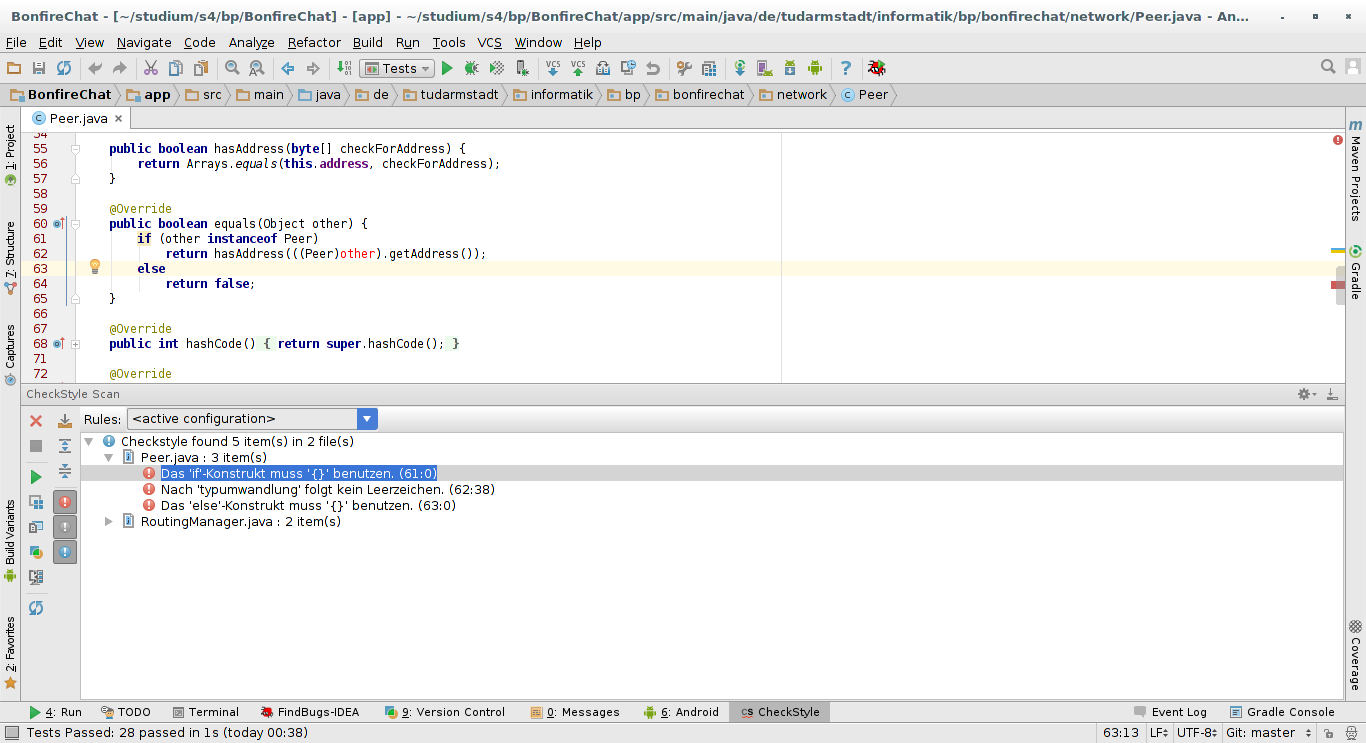
\includegraphics[width=17.5cm]{belege/checkstyle/checkstyle-idea-screenshot.png}


\clearpage
\subsection{Android Lint}

% A.1.2 Android Lint

Zusätzlich zu Checkstyle haben wir das von Google entwickelte und empfohlene \glqq Android Lint\grqq~ genutzt. Dieses Tool ist speziell für Android optimiert und erzeugt im Gegensatz zu Checkstyle weniger Warnungen bezüglich syntaktischer Programmierrichtlinien, sondern vielmehr Empfehlungen zur Verbesserung der Performance, Usability, Accessibility und Korrektheit.

Dadurch verbessert sich die Wartbarkeit, denn durch das Befolgen der im Android-Umfeld üblichen Konventionen und die Verwendung von allgemein bekannten und anerkannten Entwurfsmustern, ist der Code zukünftigen Entwicklern leichter verständlich.

Im folgenden Abschnitt befindet sich wieder ein Report, der erstellt wurde, als wir begonnen haben, \glqq Android Lint\grqq~ einzusetzen. Dann wurden initial alle Warnungen und Empfehlungen abgearbeitet (Commit 1f4733747f7a98d89e7832937d94a9ddcbdc2bd5 \glqq fixes Android Lint errors and warnings\grqq). Die Warnungen und Empfehlungen werden direkt in der von uns verwendeten Entwicklungsumgebung Android Studio angezeigt, sodass diese anschließend während der Programmierung direkt umgesetzt werden konnten. Daher ist der zweite Report, der zum Abschluss des Projekts erstellt wurde, leer.

Nach den Berichten findet sich ein Screenshot, der markierte Android Lint-Warnungen anzeigt.


\includepdf[pages=1,offset=-0.8cm 0,scale=.8,pagecommand=\subsubsection{Initialer Android Lint Report}]{anhang/partials/lint-results-1.pdf}
\includepdf[pages=2-,offset=-0.8cm 0,scale=.8,pagecommand={}]{anhang/partials/lint-results-1.pdf}

\includepdf[pages=1,offset=-0.8cm 0,scale=.8,pagecommand=\subsubsection{Finaler Android Lint Report}]{anhang/partials/lint-results-2.pdf}

\subsubsection{Screenshot von Android Lint in Android Studio}

In diesem Screenshot ist ersichtlich, wie Android Lint anmerkt, statt \glqq paddingRight\grqq~ \glqq paddingEnd\grqq~ zu verwenden. Dies ist ein Beispiel für Verbesserungen der Accessibility für Android Apps. Weiterhin angemerkt wird, dass die beiden Konstruktionen aus jeweils einem \glqq LinearLayout\grqq~ und einem \glqq ImageView\grqq~ zu einem \glqq Compound Layout\grqq~ zusammengefasst werden können.

Durch die gelbe Hinterlegung in Android Studio, welche bereits beim Tippen des Quellcodes angezeigt wird, können Android Lint Warnungen kaum übersehen werden.

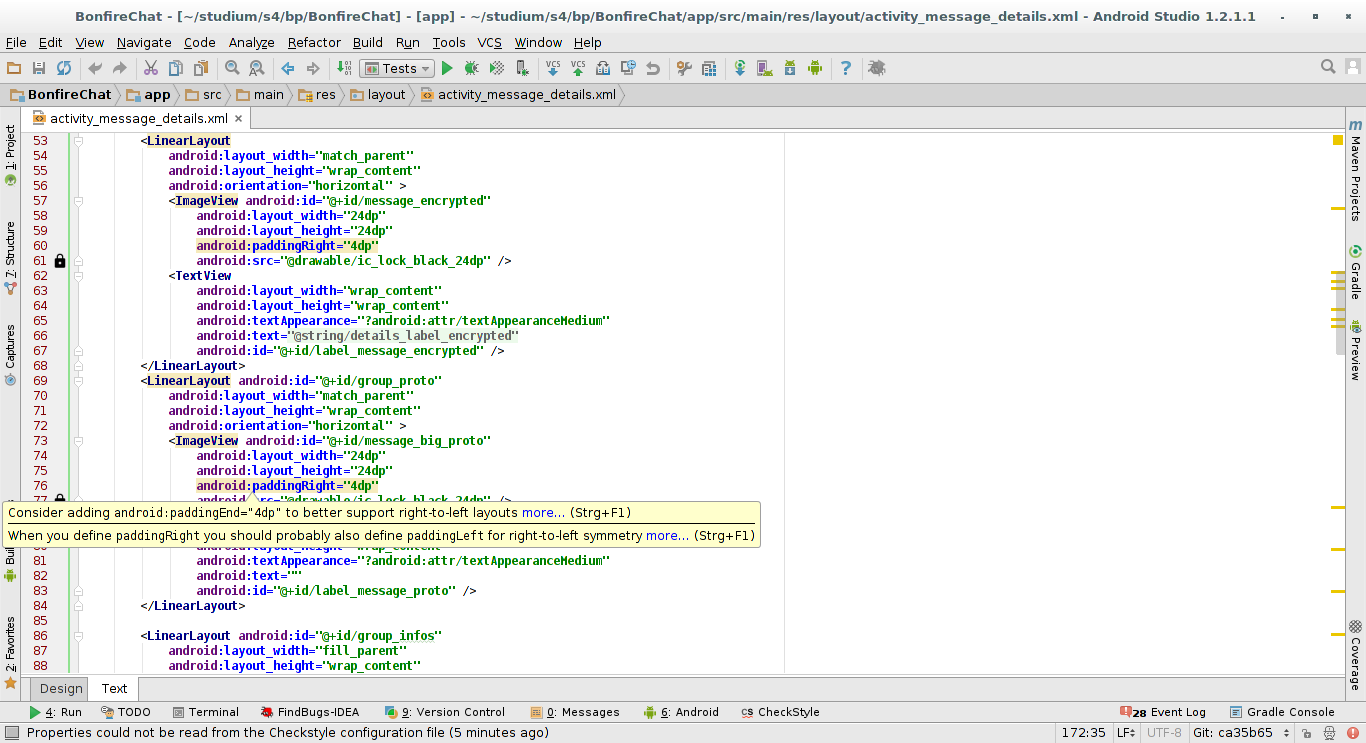
\includegraphics[width=17.5cm]{belege/lint/android-lint-screenshot.png}


\clearpage
\subsection{FindBugs}

% A.1.3 Findbugs

Um häufig auftretende Fehler zu vermeiden, haben wir \glqq FindBugs\grqq~ eingesetzt. Im Folgenden befindet sich ein Report, der erstellt wurde, als wir mit der Verwendung von FindBugs begonnen aben. Anschließend wurden alle Fehler und Warnungen in Commit e30930731deb28b4af37f4d820a163f48dcf3ff4 \glqq fixes FindBugs errors\grqq~ behoben. Da wir das Plugin FindBugs-IDEA direkt in unsere Entwicklungsumgebung integriert haben und Fehler so direkt markiert wurden, konnten Fehler ab dann direkt bei der Entwicklung vermieden werden. Bei Projektende sind keine FindBugs-Warnungen vorhanden, es kann aber kein leerer Bericht exportiert werden, da das in FindBugs-IDEA nicht vorgesehen ist.

Nach den Berichten findet sich auch für FindBugs ein Screenshot, welcher \glqq FindBugs-IDEA\grqq~ in Aktion und insbesondere die nahtlose Integration in Android Studio zeigt.

\subsubsection{FindBugs-Konfiguration}

Wir verwenden FindBugs mit folgender Gradle-Konfiguration:

\begin{lstlisting}
apply plugin: 'findbugs'

findbugs {
    excludeFilter = file("$rootProject.projectDir/config/findbugs/excludeFilter.xml")
}
\end{lstlisting}

Unsere exclude-Konfiguration sieht wie folgt aus:

\begin{lstlisting}
<?xml version="1.0" encoding="UTF-8"?>
<FindBugsFilter>
    <Match>
        <!-- ignore all issues in resource generation -->
        <Class name="~.*\.R\$.*"/>
    </Match>
    <Match>
        <Class name="~.*\.Manifest\$.*"/>
    </Match>
</FindBugsFilter>
\end{lstlisting}

\includepdf[pages=1,offset=-0.8cm 0,scale=.8,pagecommand=\subsubsection{Initialer FindBugs-Report}]{anhang/partials/findbugs-1.pdf}
\includepdf[pages=2-,offset=-0.8cm 0,scale=.8,pagecommand={}]{anhang/partials/findbugs-1.pdf}

\subsubsection{Finaler FindBugs-Report}

Es sind keine FindBugs-Fehler vorhanden, davon kann allerdings kein Bericht erstellt werden. Daher folgt hier ein Screenshot von Android Studio als Beleg.

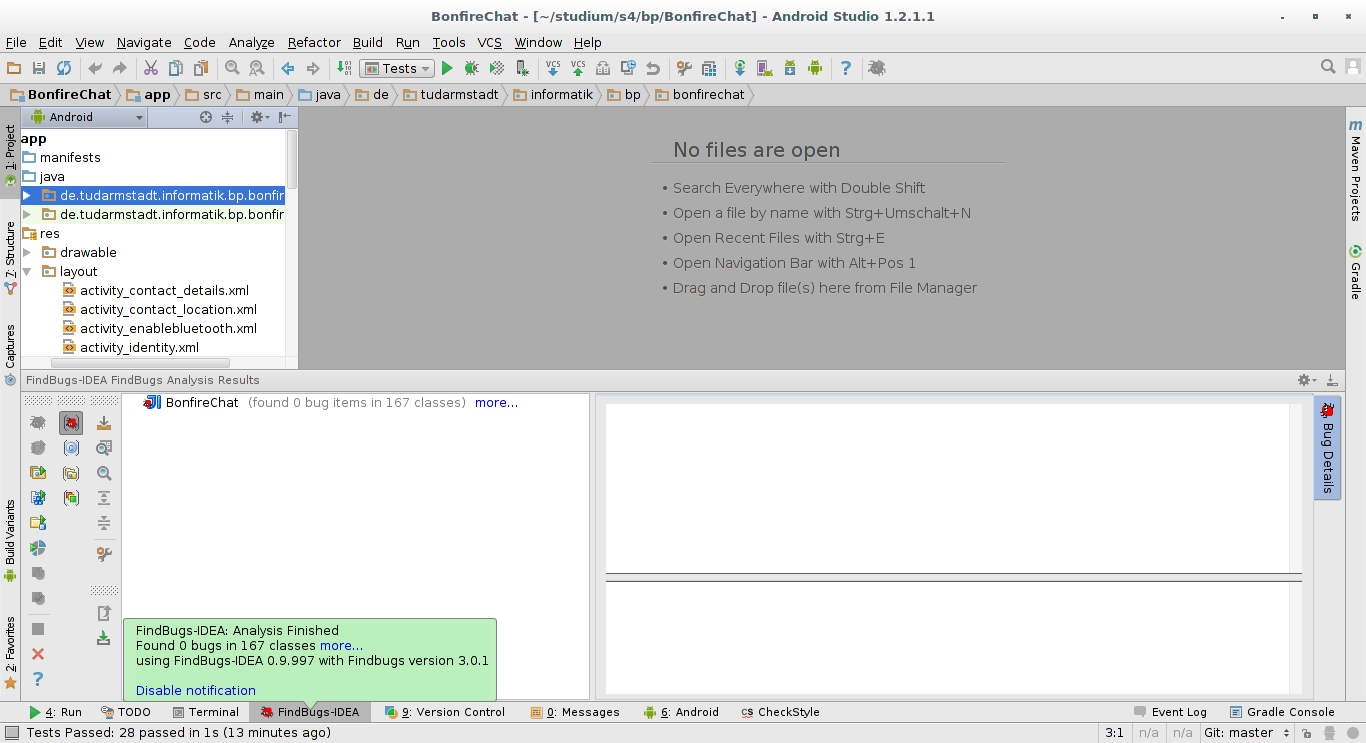
\includegraphics[width=17.5cm]{belege/findbugs/findbugs-no-warnings-screenshot.png}


\clearpage
\subsubsection{Screenshot von FindBugs-IDEA}

Im gezeigten Screenshot ist sichtbar, dass FindBugs eine Stelle im Code markiert hat, an der möglicherweise eine NullPointerException auftreten könnte. Weitere gefundene Fehler sind in der FindBugs-Ansicht unten am Bildschirm erkennbar.

Da betroffene Stellen orange unterstrichen werden und mit einer Fehlermarkierung am Rand angezeigt werden, sind sie direkt bei der Entwicklung der Anwendung ersichtlich und können umgehend behoben werden.

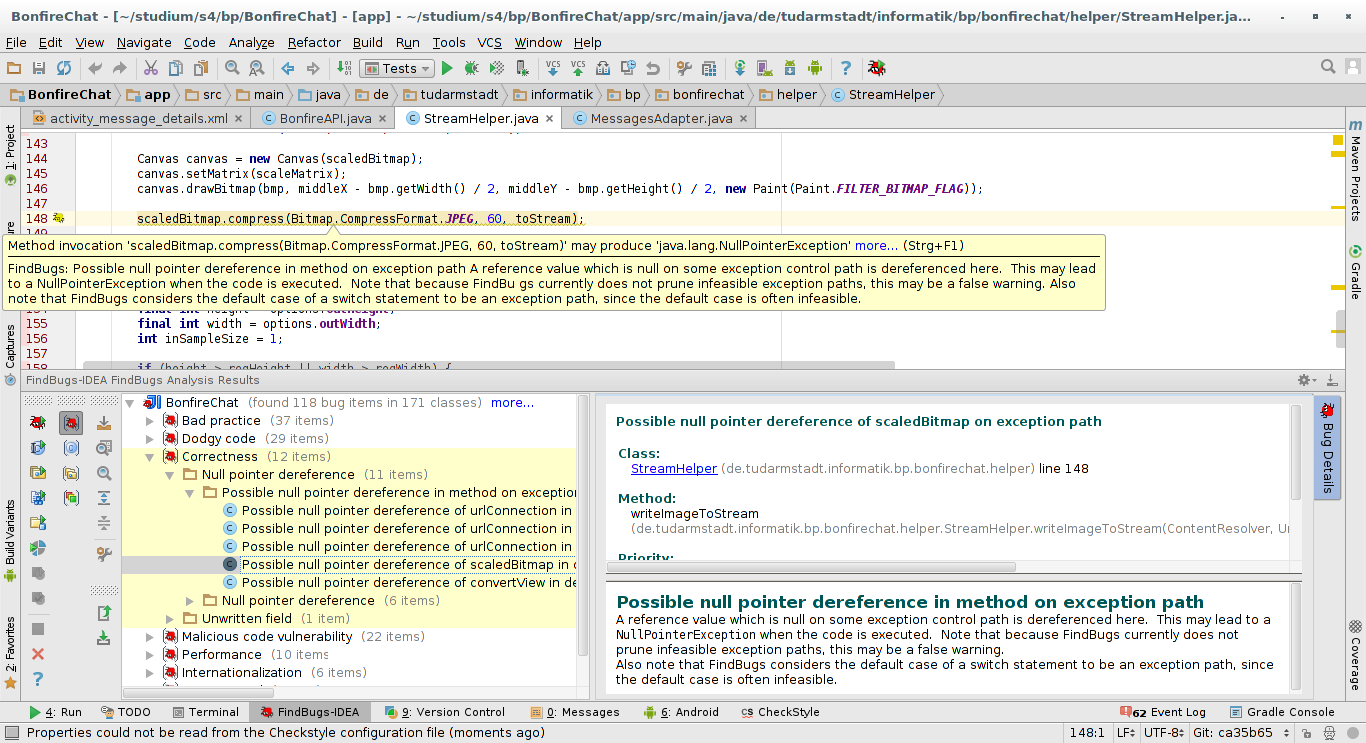
\includegraphics[width=17.5cm]{belege/findbugs/findbugs-idea-screenshot.png}

%\flushbottom


\clearpage

% ---------------------------------------------------------------------------
% Code Reviews (Einleitung)

\section{Code Reviews}

Zur Sicherstellung der Wartbarkeit durch hohe Code-Qualität wurde bei jedem
Sprint-Treffen mit dem Auftraggeber ein Code Review durchgeführt.

% ---------------------------------------------------------------------------
% Code Reviews: Checkliste

\subsection{Checkliste}


\begin{enumerate}[ 1.]
  \item Ist die Funktionalität korrekt?
  \item Sind die Klassen, Funktionen und Variablen angemessen benannt?
  \item Wurde die Klassenstruktur gut entworfen und erfüllt sie alle Anforderungen, oder sind Verbesserungen nötig?
  \item Gibt es Klassen, die aufgrund neuer Implementierungen überflüssig geworden sind?
  \item Gibt es unnötig überladene Funktionen oder Konstruktoren?
  \item Wurde die Datenbankstruktur gut entworfen?
  \item Enthält das Codeteil Funktionen, die wiederverwendet werden können? Sind diese in einer Helper-Klasse untergebracht?
  \item Wurden existierende Helper-Funktionen benutzt? Ist keine doppelte Funktionalität implementiert?
  \item Werden alle Eingabeparameter validiert?
  \item Wie beeinflusst die Funktionalität die Performance der App - Stromverbrauch, Rechenzeit und Speicherbedarf?
  \item Ist es unbedingt nötig, den Code in einem UI-Thread laufen zu lassen oder würde ein Background-Thread ausreichen?
  \item Werden alle möglichen Fehlschläge behandelt?
  \item Findet eine ``Graceful Degradation'' statt?
  \item Werden die Best Practices zur Appentwicklung, laut Android Lint, befolgt?
  \item Welche Teile können parallel ausgeführt werden?
  \item Sind die Operationen, bei denen Threadsicherheit benötigt wird, threadsicher?
  \item Ist das Layout passend für alle Bildschirmdimensionen?
  \item Haben alle Methoden und Felder die richtigen Zugriffsmodifier?
\end{enumerate}


% ---------------------------------------------------------------------------
% Code Reviews: Ergebnisse
\input{anhang/partials/codereviews.tex}


\clearpage
\section{Dokumentation}

Um die Wartung der Anwendung in Zukunft zu erleichtern, wurden die technischen Grundlagen
sowie alle wichtigen Designentscheidungen in einem Dokument festgehalten.

\input{anhang/partials/dokumentation.tex}

\clearpage
\subsection{Reviews}

Zur Sicherstellung der Qualität der Dokumentation haben wir im Abstand von etwa zwei Wochen Reviews durchgeführt. Dabei wurden insbesondere nach folgenden Problemen in der Dokumentation gesucht:

\begin{itemize}
\item Gibt es Dokumentation, die nicht mehr relevant ist und entfernt werden sollte?
\item Gibt es zentrale Konzepte, zu denen keine Dokumentation existiert?
\item Ist die Dokumentation schwer verständlich (Inhalt, Rechtschreibung)?
\end{itemize}




\subsubsection{Review am 24. Juni}

Beim Review der Dokumentation im Team wurden keine Abweichungen zwischen Code und Dokumentation festgestellt.


\subsubsection{Review am 8. Juli}

Beim Review der Dokumentation im Team wurden keine Abweichungen zwischen Code und Dokumentation festgestellt.


\subsubsection{Review am 22. Juli}

Beim Review der Dokumentation im Team wurden keine Abweichungen zwischen Code und Dokumentation festgestellt.


\subsubsection{Review am 5. August}

Beim Review der Dokumentation im Team wurden keine Abweichungen zwischen Code und Dokumentation festgestellt.


\subsubsection{Review am 18. August}

Beim Review der Dokumentation im Team wurden keine Abweichungen zwischen Code und Dokumentation festgestellt.


\subsubsection{Review am 2. September}

Beim Review der Dokumentation im Team wurden keine Abweichungen zwischen Code und Dokumentation festgestellt.


\subsubsection{Review am 14. September}

Beim Review der Dokumentation im Team wurden keine Abweichungen zwischen Code und Dokumentation festgestellt.


\subsubsection{Review am 25. September}

Beim Review der Dokumentation im Team wurden keine Abweichungen zwischen Code und Dokumentation festgestellt.








% ---------------------------------------------------------------------------
% Automatisierte Tests: (Einleitung)

\clearpage
\section{Automatisierte Tests}

Es wurden JUnit-Tests für die automatisiert testbaren Codeteile durchgeführt.
Im Folgenden findet sich zunächst eine Liste aller Tests sowie der Testergebnisse,
außerdem das Ergebnis der Test-Coverage-Analyse, aufgeschlüsselt nach Packages.

Wie bereits im QS-Dokument beschrieben, war ein Testen des UI- und Netzwerkcodes
(Packages bonfirechat.network und bonfirechat.ui)
mit dem JUnit-Framework nicht möglich, da die Android-Klassenbibliothek dort nicht
zur Verfügung steht. Das gleiche gilt für die Datenbankklasse, da diese von einer
Android-internen Klasse erbt. Daher konnte auch die Klasse bonfire.data.BonfireData
nicht mit automatisierten Tests versehen werden.

Zusammenfassend gilt, dass wir automatisierte Tests für alle Methoden geschrieben haben,
die
\begin{itemize}
\item keine Klassen der Android-Klassenbibliothek verwenden,
\item Klassen der Android-Klassenbibliothek nur als Parameter übergeben bekommen,
sodass wir stattdessen mit Mockito erstellte Mock-Objekte übergeben können, oder
\item mit vertretbarem Aufwand angepasst werden konnten, sodass der vorhergehende Punkt zutrifft.
\end{itemize}

% ---------------------------------------------------------------------------
% Automatisierte Tests: Javadoc-Testplan

\includepdf[pages=1,scale=.8,pagecommand=\subsection{Testplan}]{anhang/partials/javadoc.pdf}
\includepdf[pages=2-,scale=.8,pagecommand={}]{anhang/partials/javadoc.pdf}

% ---------------------------------------------------------------------------
% Automatisierte Tests: Ergebnisse

\includepdf[pages=1,offset=-0.8cm 0,scale=.8,pagecommand=\subsection{Ergebnisse}]{anhang/partials/junit.pdf}
\includepdf[pages=2-,offset=-0.8cm 0,scale=.8,pagecommand={}]{anhang/partials/junit.pdf}


% ---------------------------------------------------------------------------
% Automatisierte Tests: Test Coverage

\subsection{Test Coverage}

Aufgrund der in der Einleitung zu \glqq Automatisierte Tests\grqq~ beschriebenen Probleme mit JUnit und Android können große Teile unseres Quellcodes nicht automatisiert getestet werden. Daher scheint auch die Testabdeckung relativ gering zu sein, es ist jedoch nicht möglich mehr Abdeckung zu erhalten.

\hspace{-1cm}
\includegraphics[width=19.3cm,clip=true,trim=0cm 15cm 0cm 0cm]{anhang/partials/coverage.pdf}

\clearpage

\section{Manuelle Tests der Benutzeroberfläche}

Da uns der Aufwand für die Nutzung eines Instrumented-Test-Frameworks
für das recht einfache User Interface der App unverhältnismäßig
erscheint, werden manuelle Tests anhand des folgenden Testplans
vorgenommen.

\subsection{Testplan}

Dieser Abschnitt beschreibt einen Testplan für manuelles Testen der
drahtlosen Übertragung sowie des Routing-Algorithmus.\\\\

% ----------------------------------------------------------------------

\subsubsection{N-i: Definitionen}\label{i-definitionen}

\paragraph{Allgemeine Ausgangskonfiguration der
Knoten:}\label{allgemeine-ausgangskonfiguration-der-knoten}

Ein Knoten ist, soweit nicht näher beschrieben, ein Android-Gerät, auf
dem die aktuellste Version der App eingerichtet und die initiale
Einrichtung (Eingabe eines Nicknames, dadurch Registrierung des Gerätes
mit Nickname, GCM-ID und PublicKey am Server) abgeschlossen ist.


% ----------------------------------------------------------------------
% II

\clearpage
\subsubsection{N-ii: Testfälle für die allgemeine
Übertragung}\label{ii-testfuxe4lle-fuxfcr-die-allgemeine-uxfcbertragung}

\paragraph{N-ii-1. Test der direkten Übertragung via Flooding /
Bluetooth}\label{test-der-direkten-uxfcbertragung-via-flooding-bluetooth}

\begin{longtable}{p{8cm}p{8.5cm}}
\toprule
Benutzerinteraktion & erwartetes Verhalten der App\tabularnewline
\midrule
\endhead
Auf zwei Knoten A und B, die sich in direkter Bluetooth-Reichweite
befinden, wird zunächst die Ausgangskonfiguration hergestellt,
anschließend werden in den Einstellungen alle Übertragungsverfahren
außer Bluetooth deaktiviert. Die Kontaktdaten von A werden an B
gesendet. Auf B wird eine neue Unterhaltung mit A gestartet. Auf B wird
eine Nachricht an A eingegeben und abgesendet. & B sendet die Nachricht
an alle per Bluetooth sichtbaren Geräte, insbesondere an A. Auf A wird
die Nachricht empfangen und als per Bluetooth empfangen dargestellt. A
sendet ein ACK an B, dieses wird auf B durch ein Häkchen an der
Nachricht sichtbar. Weiterhin erscheint ein Bluetooth-Icon an der
Nachricht, da die Nachricht per Bluetooth zugestellt wurde. Im Dashboard
ist erkennbar, dass die Nachricht mit Routingmodus Flooding (0x01)
versendet wurde, das ACK mit Routingmodus DSR (0x02).\tabularnewline
\bottomrule
\end{longtable}

\paragraph{N-ii-2. Test der direkten Übertragung via DSR /
Bluetooth}\label{test-der-direkten-uxfcbertragung-via-dsr-bluetooth}

\begin{longtable}{p{8cm}p{8.5cm}}
\toprule
Benutzerinteraktion & erwartetes Verhalten der App\tabularnewline
\midrule
\endhead
Nach der erfolgreichen Durchführung von Test 1 wird eine weitere
Nachricht von B an A gesendet, sowie eine Nachricht von A an B. & Nach
Test 1 ist den Geräten A und B der schnellste Pfad zum jeweils anderen
Gerät bekannt. Daher sendet B die Nachricht nicht per Routingmodus
Flooding (0x01), sondern per Dynamic Source Routing (0x02), also unter
der Angabe der gewünschten Übertragungspfades. Daher wird die Nachricht
nur an Gerät A gesendet. Darüber hinaus identisch zu Test
1.\tabularnewline
\bottomrule
\end{longtable}

\paragraph{N-ii-3. Test der direkten Übertragung via Server / Google Cloud
Messaging}\label{test-der-direkten-uxfcbertragung-via-server-google-cloud-messaging}

\begin{longtable}{p{8cm}p{8.5cm}}
\toprule
Benutzerinteraktion & erwartetes Verhalten der App\tabularnewline
\midrule
\endhead
Auf zwei Knoten A und B, die eine funktionierende Internetverbindung
haben, wird zunächst die Ausgangskonfiguration hergestellt, anschließend
werden in den Einstellungen alle Übertragungsverfahren außer ``mobile
Daten / Wifi'' (Übertragung per Cloud) deaktiviert. Die Kontaktdaten von
A werden an B gesendet. Auf B wird eine neue Unterhaltung mit A
gestartet. Auf B wird eine Nachricht an A eingegeben und abgesendet. & B
sendet die Nachricht per HTTP an den Server, welcher sie per GCM an
Gerät A weiterleitet. Auf A wird die Nachricht empfangen und als per
Cloud empfangen dargestellt. A sendet ein ACK an B, dieses wird auf B
durch ein Häkchen an der Nachricht sichtbar. Weiterhin erscheint ein
Cloud-Icon an der Nachricht, da die Nachricht per Cloud zugestellt
wurde. Im Dashboard ist erkennbar, dass die Nachricht mit Routingmodus
Flooding (0x01) versendet wurde, das ACK mit Routingmodus DSR
(0x02).\tabularnewline
\bottomrule
\end{longtable}


% ----------------------------------------------------------------------
% III

\clearpage
\subsubsection{N-iii: Testfälle für Wegfindung per Flooding und einfaches
Routing}\label{iii-testfuxe4lle-fuxfcr-wegfindung-per-flooding-und-einfaches-routing}

In diesen Tests werden folgende Teile des Routing getestet: * Finden des
schnellsten Pfades: Flooding an alle Knoten sowie ACK auf dem Pfad, auf
dem die Nachricht den Empfänger zuerst erreicht (= schnellster Pfad) *
Speichern des schnellsten Pfades zu einem Empfänger * Verwenden des
gespeicherten schnellsten Pfades für künftige Nachrichten

\paragraph{N-iii-1. Bluetooth-Wegfindung - Flooding mit drei
Knoten}\label{bluetooth-wegfindung---flooding-mit-drei-knoten}

\begin{longtable}{p{8cm}p{8.5cm}}
\toprule
Benutzerinteraktion & erwartetes Verhalten der App\tabularnewline
\midrule
\endhead
Auf drei Knoten A, B und C werden alle Übertragungsverfahren außer
Bluetooth deaktiviert. Die Kontaktdetails von C werden an A gesendet.
Die Knoten werden räumlich so angeordnet, dass eine Bluetoothverbindung
zwischen A und B sowie zwischen B und C möglich ist, nicht jedoch
zwischen A und C. Auf A wird eine Unterhaltung mit C begonnen und eine
Nachricht an C gesendet. & Nachricht u. ACK kommen an,
etc.\tabularnewline
\bottomrule
\end{longtable}

\paragraph{N-iii-2. Bluetooth-Wegfindung zum nächsten Knoten mit
Internetverbindung}\label{bluetooth-wegfindung-zum-nuxe4chsten-knoten-mit-internetverbindung}

\begin{longtable}{p{8cm}p{8.5cm}}
\toprule
Benutzerinteraktion & erwartetes Verhalten der App\tabularnewline
\midrule
\endhead
Knoten A, B und C werden wie in Testfall III.1 vorbereitet. Auf Knoten C
wird zusätzlich die Übertragung per Cloud aktiviert. Auf einem weiteren
Knoten D wird nur die Übertragung per Cloud aktiviert. Es wird
sichergestellt, dass C und D mit dem Internet verbunden sind. Die
Kontaktdetails von D werden an A gesendet. A beginnt eine Unterhaltung
mit D und sendet die Nachricht ``alpha'' an D. Nach Erhalt der Nachricht
``alpha'' sendet A eine weitere Nachricht ``beta''. & Die Nachricht
``alpha'' kommt per Flooding über B, C und Server bei D an, ACK ``für
alpha'' geht auf direktem Pfad (D-Server-C-B-A) per DSR zurück an A. Die
Nachricht ``beta'' wird auf direktem Pfad (A-B-C-Server-D) per DSR an D
gesendet, ACK ``für beta'' wie ACK ``für alpha''. Die empfangenen und
weitergeleiteten Nachrichten und ihre Pfade sind entsprechend im
Dashboard ersichtlich.\tabularnewline
\bottomrule
\end{longtable}

\paragraph{N-iii-3.}\label{section}

TODO Test beschreiben




% ------------------------------------------------------------------------
% IV

\clearpage
\subsubsection{N-iv: Testfälle für sich verändernde
Routen}\label{iv-testfuxe4lle-fuxfcr-sich-veruxe4ndernde-routen}

In diesen Tests wird überprüft, ob der Routingalgorithmus bei
ausfallenden Pfaden korrekt reagiert.

\paragraph{\texorpdfstring{N-iv-1. ``Abreißende''
Bluetooth-Verbindung}{N-iv-1. Abreißende Bluetooth-Verbindung}}\label{abreiuxdfende-bluetooth-verbindung}

\begin{longtable}{p{8cm}p{8.5cm}}
\toprule
Benutzerinteraktion & erwartetes Verhalten der App\tabularnewline
\midrule
\endhead
Auf drei Knoten A wird nur Bluetooth aktiviert, auf B wird GCM und
Bluetooth aktiviert. Von A wird eine Nachricht ``alpha'' an B gesendet.
Nachdem diese zugestellt und acknowledged wurde, wird eine weitere
Nachricht ``beta'' von A and B gesendet. Danach wird A räumlich so weit
vom B entfernt, dass keine Bluetooth-Übertragung mehr möglich ist.
Weiterhin wird auf A die Übertragung per GCM aktiviert. Anschließend
wird eine weitere Nachricht ``gamma'' von A and B gesendet. & Die
Nachricht ``alpha'' wird per Flooding gesendet, B sendet per DSR ein ACK
``für alpha'' zurück. Danach hat A den Pfad zu B gespeichert und die
Nachricht ``beta'' wird direkt per DSR an B gesendet. Die Nachricht
``gamma'' wird auch versucht per DSR direkt via Bluetooth an B zu
senden. Da dies fehlschlägt, wird beim Retry nach 20 Sekunden versucht,
``gamma'' per Flooding zuzustellen. Dies erfolgt dann über GCM. Das ACK
``für gamma'' von B an A erfolgt dann wiederum per DSR.\tabularnewline
\bottomrule
\end{longtable}



% ------------------------------------------------------------------------
% V

\clearpage
\subsubsection{N-v: Testfälle für Störeinflüsse im
Netzwerk}\label{v-testfuxe4lle-fuxfcr-stuxf6reinfluxfcsse-im-netzwerk}

Hier soll überprüft werden, wie sich die App bei äußeren Störeinflüssen
auf Netzwerkebene, also zum Beispiel während einer während der
Datenübertragung abreißenden Verbindung, verhält. Es soll sichergestellt
sein, dass stets angemessen reagiert wird und sowohl die App nicht
abstürzt als auch der Benutzer sinnvolle Fehlermeldungen erhält.

Da dies teilweise sporadische Fehler sind, welche sich schwer
reproduzieren lassen, ist die Aussagekraft der folgenden Tests leider
nur bedingt gegeben.

\paragraph{\texorpdfstring{N-v-1. ``Socket wird unerwartet während der
Verbindung
geschlossen''}{N-v-1. Socket wird unerwartet während der Verbindung geschlossen}}\label{socket-wird-unerwartet-wuxe4hrend-der-verbindung-geschlossen}

\begin{longtable}{p{8cm}p{8.5cm}}
\toprule
Benutzerinteraktion & erwartetes Verhalten der App\tabularnewline
\midrule
\endhead
\bottomrule
\end{longtable}

\paragraph{N-v-2. Benutzer schaltet Bluetooth im Telefon
aus}\label{benutzer-schaltet-bluetooth-im-telefon-aus}

\begin{longtable}{p{8cm}p{8.5cm}}
\toprule
Benutzerinteraktion & erwartetes Verhalten der App\tabularnewline
\midrule
\endhead
\bottomrule
\end{longtable}


\input{anhang/partials/manuelle-tests-ui-reports.tex}


\clearpage
\section{Manueller Test für Routing und Datenübertragungs-Protokolle}

Ebenso wie bei den manuellen Tests der Benutzeroberfläche ist es kaum möglich, das Netzwerkverhalten der Anwendung automatisiert zu testen, da dafür physikalische Eigenschaften der Funkübertragung simuliert werden müssten. Wir haben daher manuelle Tests anhand des folgenden Testplans vorgenommen.

\subsection{Testplan}

Dieser Abschnitt beschreibt einen Testplan für manuelles Testen der
drahtlosen Übertragung sowie des Routing-Algorithmus.\\\\

% ----------------------------------------------------------------------

\subsubsection{N-i: Definitionen}\label{i-definitionen}

\paragraph{Allgemeine Ausgangskonfiguration der
Knoten:}\label{allgemeine-ausgangskonfiguration-der-knoten}

Ein Knoten ist, soweit nicht näher beschrieben, ein Android-Gerät, auf
dem die aktuellste Version der App eingerichtet und die initiale
Einrichtung (Eingabe eines Nicknames, dadurch Registrierung des Gerätes
mit Nickname, GCM-ID und PublicKey am Server) abgeschlossen ist.


% ----------------------------------------------------------------------
% II

\clearpage
\subsubsection{N-ii: Testfälle für die allgemeine
Übertragung}\label{ii-testfuxe4lle-fuxfcr-die-allgemeine-uxfcbertragung}

\paragraph{N-ii-1. Test der direkten Übertragung via Flooding /
Bluetooth}\label{test-der-direkten-uxfcbertragung-via-flooding-bluetooth}

\begin{longtable}{p{8cm}p{8.5cm}}
\toprule
Benutzerinteraktion & erwartetes Verhalten der App\tabularnewline
\midrule
\endhead
Auf zwei Knoten A und B, die sich in direkter Bluetooth-Reichweite
befinden, wird zunächst die Ausgangskonfiguration hergestellt,
anschließend werden in den Einstellungen alle Übertragungsverfahren
außer Bluetooth deaktiviert. Die Kontaktdaten von A werden an B
gesendet. Auf B wird eine neue Unterhaltung mit A gestartet. Auf B wird
eine Nachricht an A eingegeben und abgesendet. & B sendet die Nachricht
an alle per Bluetooth sichtbaren Geräte, insbesondere an A. Auf A wird
die Nachricht empfangen und als per Bluetooth empfangen dargestellt. A
sendet ein ACK an B, dieses wird auf B durch ein Häkchen an der
Nachricht sichtbar. Weiterhin erscheint ein Bluetooth-Icon an der
Nachricht, da die Nachricht per Bluetooth zugestellt wurde. Im Dashboard
ist erkennbar, dass die Nachricht mit Routingmodus Flooding (0x01)
versendet wurde, das ACK mit Routingmodus DSR (0x02).\tabularnewline
\bottomrule
\end{longtable}

\paragraph{N-ii-2. Test der direkten Übertragung via DSR /
Bluetooth}\label{test-der-direkten-uxfcbertragung-via-dsr-bluetooth}

\begin{longtable}{p{8cm}p{8.5cm}}
\toprule
Benutzerinteraktion & erwartetes Verhalten der App\tabularnewline
\midrule
\endhead
Nach der erfolgreichen Durchführung von Test 1 wird eine weitere
Nachricht von B an A gesendet, sowie eine Nachricht von A an B. & Nach
Test 1 ist den Geräten A und B der schnellste Pfad zum jeweils anderen
Gerät bekannt. Daher sendet B die Nachricht nicht per Routingmodus
Flooding (0x01), sondern per Dynamic Source Routing (0x02), also unter
der Angabe der gewünschten Übertragungspfades. Daher wird die Nachricht
nur an Gerät A gesendet. Darüber hinaus identisch zu Test
1.\tabularnewline
\bottomrule
\end{longtable}

\paragraph{N-ii-3. Test der direkten Übertragung via Server / Google Cloud
Messaging}\label{test-der-direkten-uxfcbertragung-via-server-google-cloud-messaging}

\begin{longtable}{p{8cm}p{8.5cm}}
\toprule
Benutzerinteraktion & erwartetes Verhalten der App\tabularnewline
\midrule
\endhead
Auf zwei Knoten A und B, die eine funktionierende Internetverbindung
haben, wird zunächst die Ausgangskonfiguration hergestellt, anschließend
werden in den Einstellungen alle Übertragungsverfahren außer ``mobile
Daten / Wifi'' (Übertragung per Cloud) deaktiviert. Die Kontaktdaten von
A werden an B gesendet. Auf B wird eine neue Unterhaltung mit A
gestartet. Auf B wird eine Nachricht an A eingegeben und abgesendet. & B
sendet die Nachricht per HTTP an den Server, welcher sie per GCM an
Gerät A weiterleitet. Auf A wird die Nachricht empfangen und als per
Cloud empfangen dargestellt. A sendet ein ACK an B, dieses wird auf B
durch ein Häkchen an der Nachricht sichtbar. Weiterhin erscheint ein
Cloud-Icon an der Nachricht, da die Nachricht per Cloud zugestellt
wurde. Im Dashboard ist erkennbar, dass die Nachricht mit Routingmodus
Flooding (0x01) versendet wurde, das ACK mit Routingmodus DSR
(0x02).\tabularnewline
\bottomrule
\end{longtable}


% ----------------------------------------------------------------------
% III

\clearpage
\subsubsection{N-iii: Testfälle für Wegfindung per Flooding und einfaches
Routing}\label{iii-testfuxe4lle-fuxfcr-wegfindung-per-flooding-und-einfaches-routing}

In diesen Tests werden folgende Teile des Routing getestet: * Finden des
schnellsten Pfades: Flooding an alle Knoten sowie ACK auf dem Pfad, auf
dem die Nachricht den Empfänger zuerst erreicht (= schnellster Pfad) *
Speichern des schnellsten Pfades zu einem Empfänger * Verwenden des
gespeicherten schnellsten Pfades für künftige Nachrichten

\paragraph{N-iii-1. Bluetooth-Wegfindung - Flooding mit drei
Knoten}\label{bluetooth-wegfindung---flooding-mit-drei-knoten}

\begin{longtable}{p{8cm}p{8.5cm}}
\toprule
Benutzerinteraktion & erwartetes Verhalten der App\tabularnewline
\midrule
\endhead
Auf drei Knoten A, B und C werden alle Übertragungsverfahren außer
Bluetooth deaktiviert. Die Kontaktdetails von C werden an A gesendet.
Die Knoten werden räumlich so angeordnet, dass eine Bluetoothverbindung
zwischen A und B sowie zwischen B und C möglich ist, nicht jedoch
zwischen A und C. Auf A wird eine Unterhaltung mit C begonnen und eine
Nachricht an C gesendet. & Nachricht u. ACK kommen an,
etc.\tabularnewline
\bottomrule
\end{longtable}

\paragraph{N-iii-2. Bluetooth-Wegfindung zum nächsten Knoten mit
Internetverbindung}\label{bluetooth-wegfindung-zum-nuxe4chsten-knoten-mit-internetverbindung}

\begin{longtable}{p{8cm}p{8.5cm}}
\toprule
Benutzerinteraktion & erwartetes Verhalten der App\tabularnewline
\midrule
\endhead
Knoten A, B und C werden wie in Testfall III.1 vorbereitet. Auf Knoten C
wird zusätzlich die Übertragung per Cloud aktiviert. Auf einem weiteren
Knoten D wird nur die Übertragung per Cloud aktiviert. Es wird
sichergestellt, dass C und D mit dem Internet verbunden sind. Die
Kontaktdetails von D werden an A gesendet. A beginnt eine Unterhaltung
mit D und sendet die Nachricht ``alpha'' an D. Nach Erhalt der Nachricht
``alpha'' sendet A eine weitere Nachricht ``beta''. & Die Nachricht
``alpha'' kommt per Flooding über B, C und Server bei D an, ACK ``für
alpha'' geht auf direktem Pfad (D-Server-C-B-A) per DSR zurück an A. Die
Nachricht ``beta'' wird auf direktem Pfad (A-B-C-Server-D) per DSR an D
gesendet, ACK ``für beta'' wie ACK ``für alpha''. Die empfangenen und
weitergeleiteten Nachrichten und ihre Pfade sind entsprechend im
Dashboard ersichtlich.\tabularnewline
\bottomrule
\end{longtable}

\paragraph{N-iii-3.}\label{section}

TODO Test beschreiben




% ------------------------------------------------------------------------
% IV

\clearpage
\subsubsection{N-iv: Testfälle für sich verändernde
Routen}\label{iv-testfuxe4lle-fuxfcr-sich-veruxe4ndernde-routen}

In diesen Tests wird überprüft, ob der Routingalgorithmus bei
ausfallenden Pfaden korrekt reagiert.

\paragraph{\texorpdfstring{N-iv-1. ``Abreißende''
Bluetooth-Verbindung}{N-iv-1. Abreißende Bluetooth-Verbindung}}\label{abreiuxdfende-bluetooth-verbindung}

\begin{longtable}{p{8cm}p{8.5cm}}
\toprule
Benutzerinteraktion & erwartetes Verhalten der App\tabularnewline
\midrule
\endhead
Auf drei Knoten A wird nur Bluetooth aktiviert, auf B wird GCM und
Bluetooth aktiviert. Von A wird eine Nachricht ``alpha'' an B gesendet.
Nachdem diese zugestellt und acknowledged wurde, wird eine weitere
Nachricht ``beta'' von A and B gesendet. Danach wird A räumlich so weit
vom B entfernt, dass keine Bluetooth-Übertragung mehr möglich ist.
Weiterhin wird auf A die Übertragung per GCM aktiviert. Anschließend
wird eine weitere Nachricht ``gamma'' von A and B gesendet. & Die
Nachricht ``alpha'' wird per Flooding gesendet, B sendet per DSR ein ACK
``für alpha'' zurück. Danach hat A den Pfad zu B gespeichert und die
Nachricht ``beta'' wird direkt per DSR an B gesendet. Die Nachricht
``gamma'' wird auch versucht per DSR direkt via Bluetooth an B zu
senden. Da dies fehlschlägt, wird beim Retry nach 20 Sekunden versucht,
``gamma'' per Flooding zuzustellen. Dies erfolgt dann über GCM. Das ACK
``für gamma'' von B an A erfolgt dann wiederum per DSR.\tabularnewline
\bottomrule
\end{longtable}



% ------------------------------------------------------------------------
% V

\clearpage
\subsubsection{N-v: Testfälle für Störeinflüsse im
Netzwerk}\label{v-testfuxe4lle-fuxfcr-stuxf6reinfluxfcsse-im-netzwerk}

Hier soll überprüft werden, wie sich die App bei äußeren Störeinflüssen
auf Netzwerkebene, also zum Beispiel während einer während der
Datenübertragung abreißenden Verbindung, verhält. Es soll sichergestellt
sein, dass stets angemessen reagiert wird und sowohl die App nicht
abstürzt als auch der Benutzer sinnvolle Fehlermeldungen erhält.

Da dies teilweise sporadische Fehler sind, welche sich schwer
reproduzieren lassen, ist die Aussagekraft der folgenden Tests leider
nur bedingt gegeben.

\paragraph{\texorpdfstring{N-v-1. ``Socket wird unerwartet während der
Verbindung
geschlossen''}{N-v-1. Socket wird unerwartet während der Verbindung geschlossen}}\label{socket-wird-unerwartet-wuxe4hrend-der-verbindung-geschlossen}

\begin{longtable}{p{8cm}p{8.5cm}}
\toprule
Benutzerinteraktion & erwartetes Verhalten der App\tabularnewline
\midrule
\endhead
\bottomrule
\end{longtable}

\paragraph{N-v-2. Benutzer schaltet Bluetooth im Telefon
aus}\label{benutzer-schaltet-bluetooth-im-telefon-aus}

\begin{longtable}{p{8cm}p{8.5cm}}
\toprule
Benutzerinteraktion & erwartetes Verhalten der App\tabularnewline
\midrule
\endhead
\bottomrule
\end{longtable}


\subsection{Durchführung des manuellen Netzwerk-Testplans vom 30. August 2015}

\textbf{Durchgeführt von:} Matthias Hofmann

\textbf{Änderungen vorgenommen in Commit:} keine Änderungen nötig

\paragraph{Teil N-ii Testfälle für die allgemeine Übertragung}

\paragraph{Test N-ii.1 Test der direkten Übertragung via Flooding / Bluetooth}

Der Test war erfolgreich.

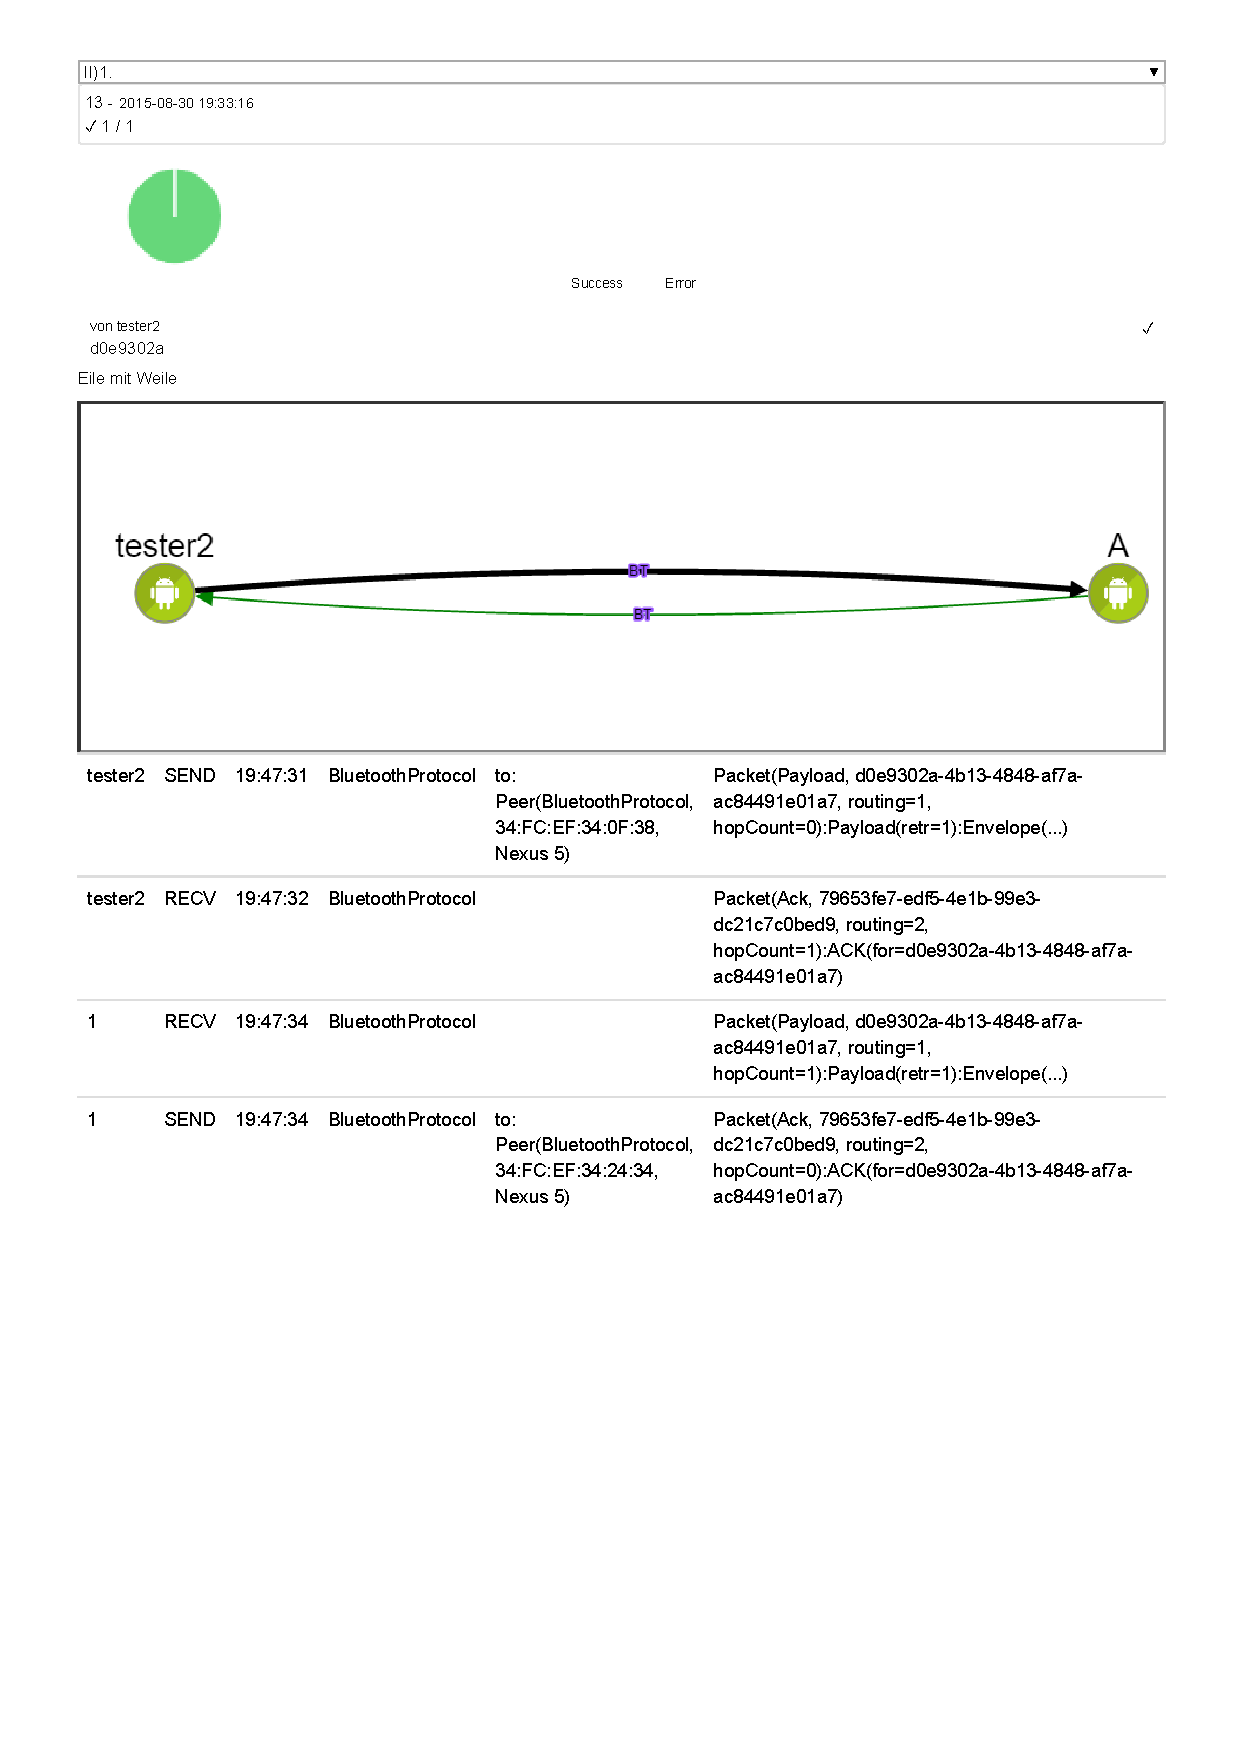
\includegraphics[trim=0 180 0 0,clip,scale=0.8]{belege/manuelle-tests/netzwerk/Dashboardauszuege/Netzwerktest_II-1.pdf}
\clearpage

\paragraph{Test N-ii.2 Test der direkten Übertragung via DSR / Bluetooth}

Der Test war erfolgreich.

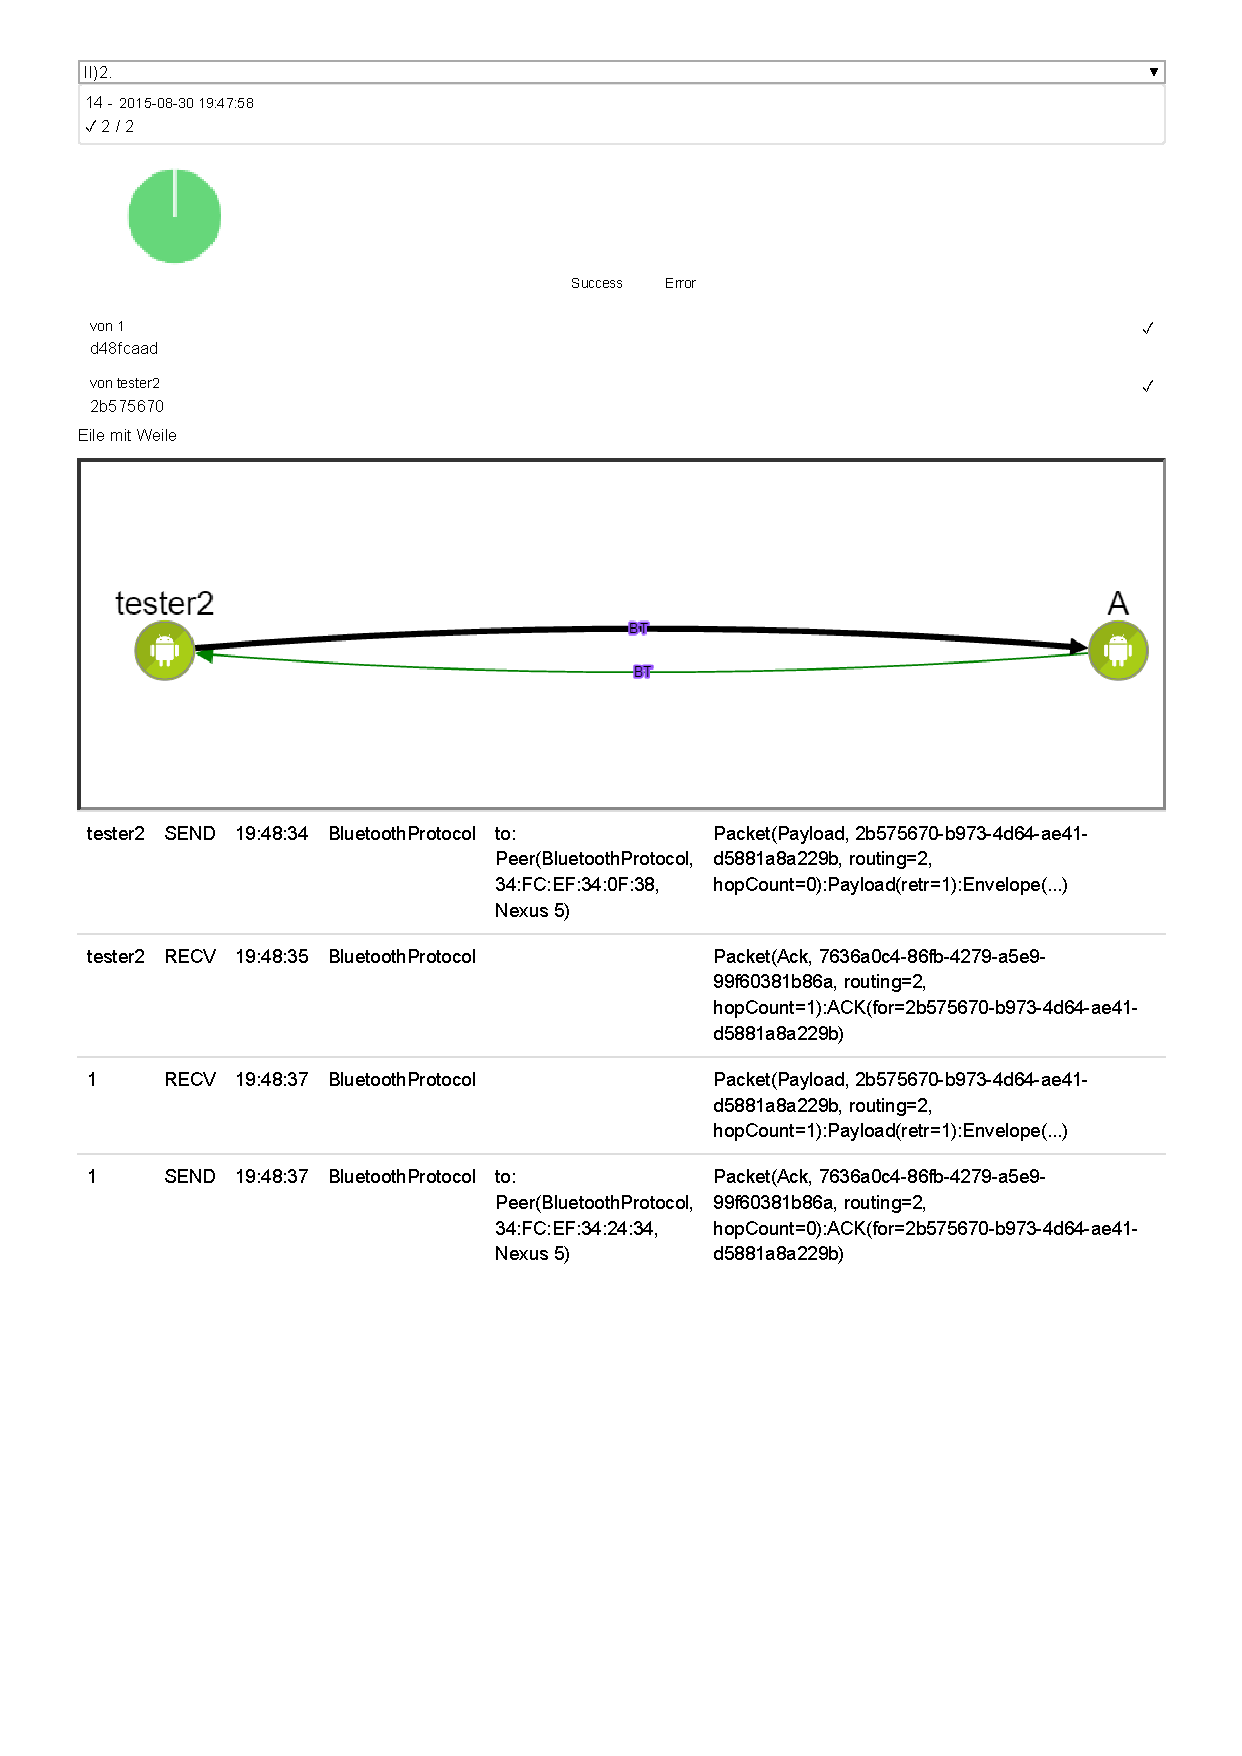
\includegraphics[trim=0 120 0 0,clip,scale=0.8]{belege/manuelle-tests/netzwerk/Dashboardauszuege/Netzwerktest_II-2a.pdf}
\clearpage
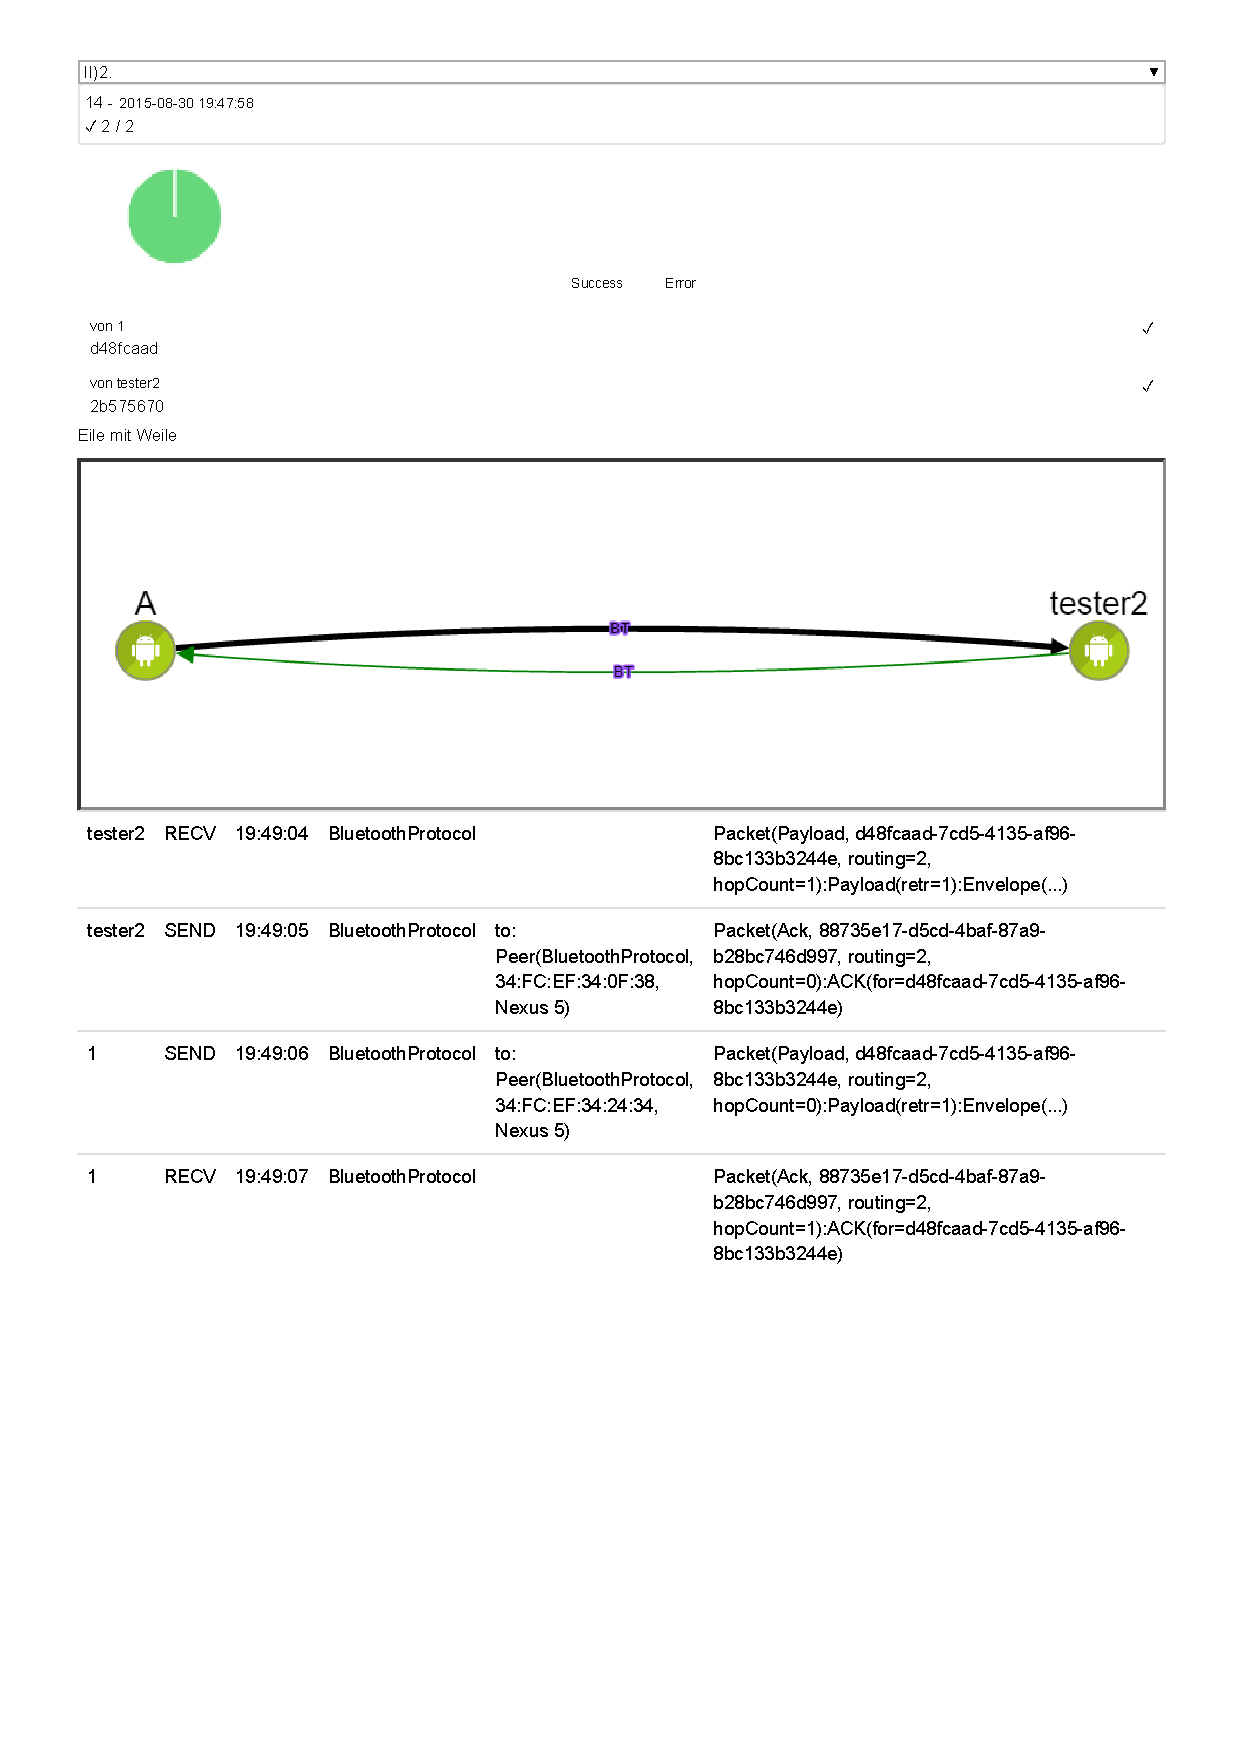
\includegraphics[trim=0 120 0 0,clip,scale=0.8]{belege/manuelle-tests/netzwerk/Dashboardauszuege/Netzwerktest_II-2b.pdf}
\clearpage

\paragraph{Test N-ii.3 Test der direkten Übertragung via Server / Google Cloud Messaging}

Der Test war erfolgreich.

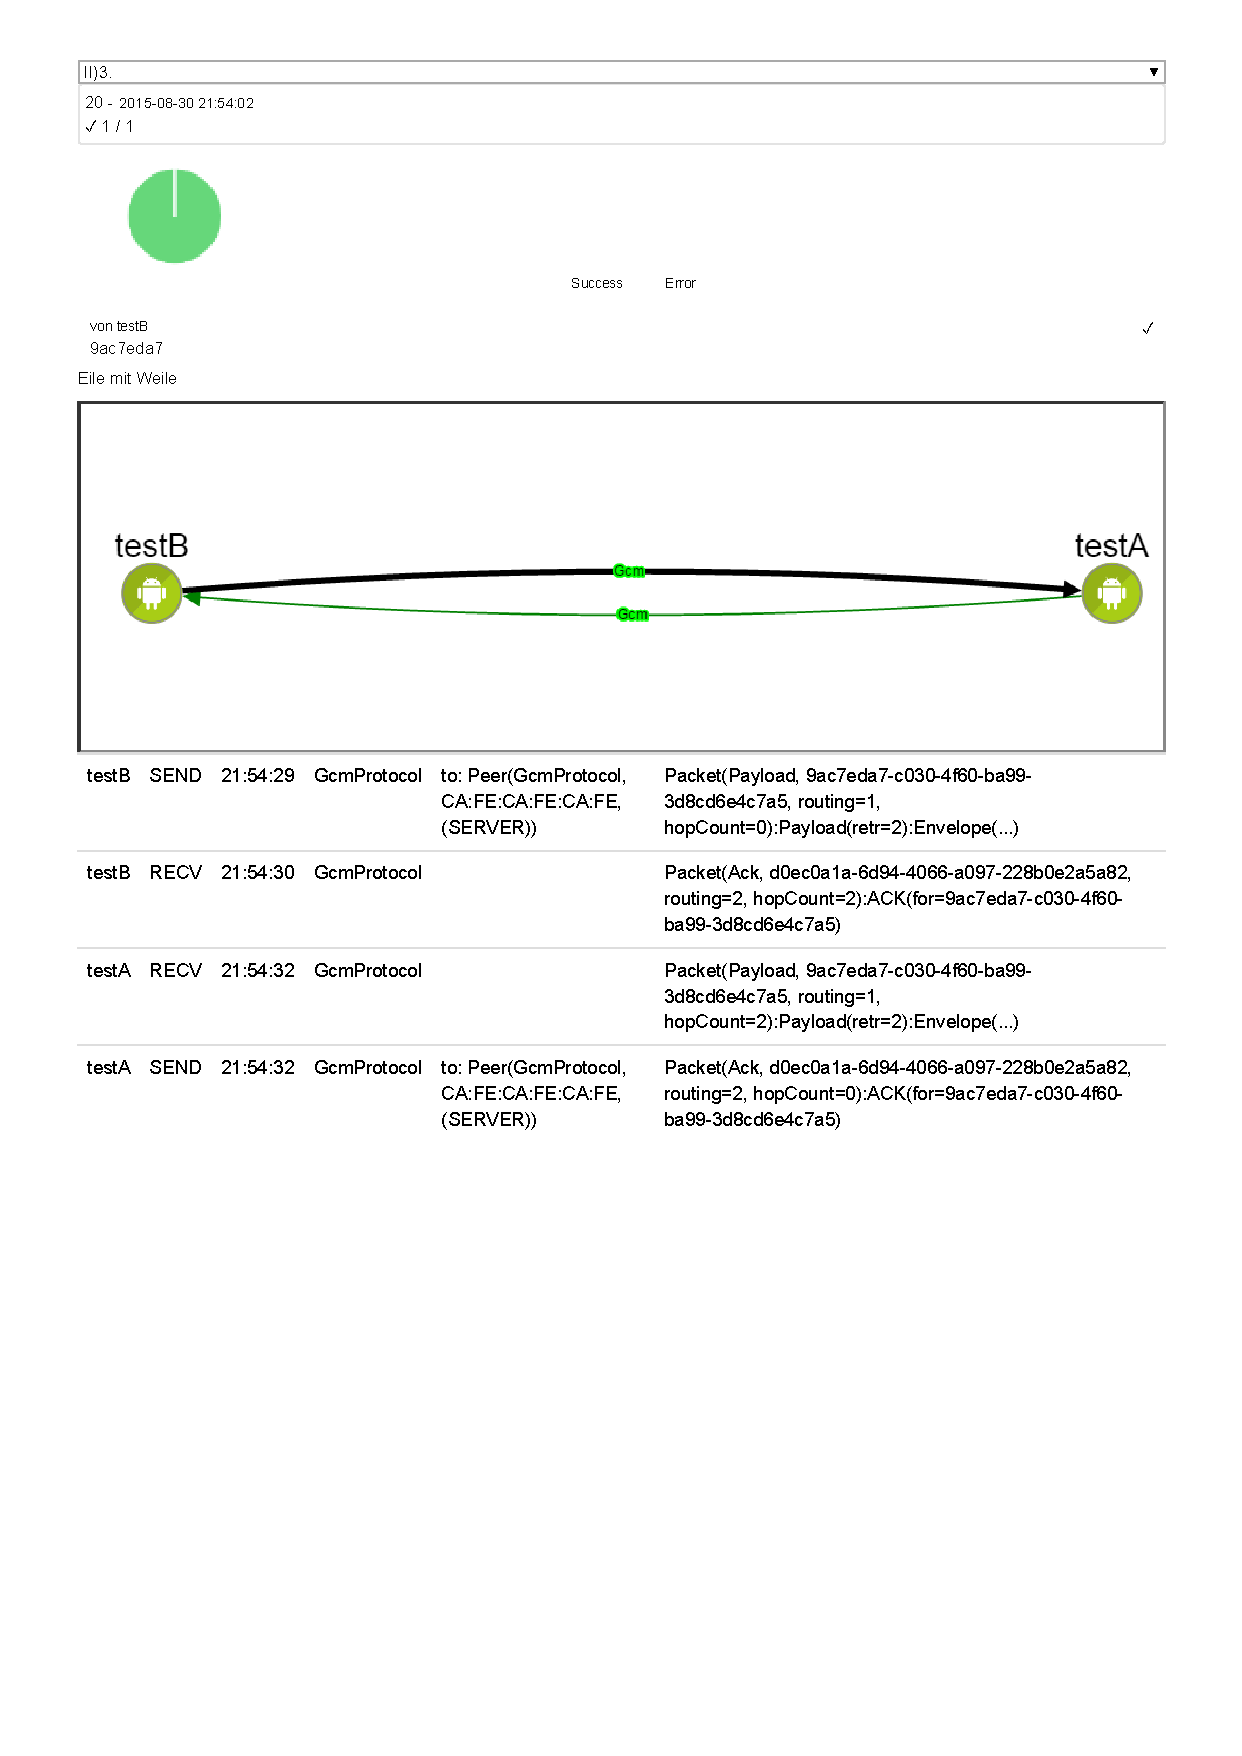
\includegraphics[trim=0 120 0 0,clip,scale=0.8]{belege/manuelle-tests/netzwerk/Dashboardauszuege/Netzwerktest_II-3.pdf}
\clearpage


\paragraph{Teil N-iii Testfälle für Wegfindung per Flooding und einfaches Routing}

\paragraph{Test N-iii.1 Bluetooth-Wegfindung - Flooding mit drei Knoten}

Der Test war erfolgreich.

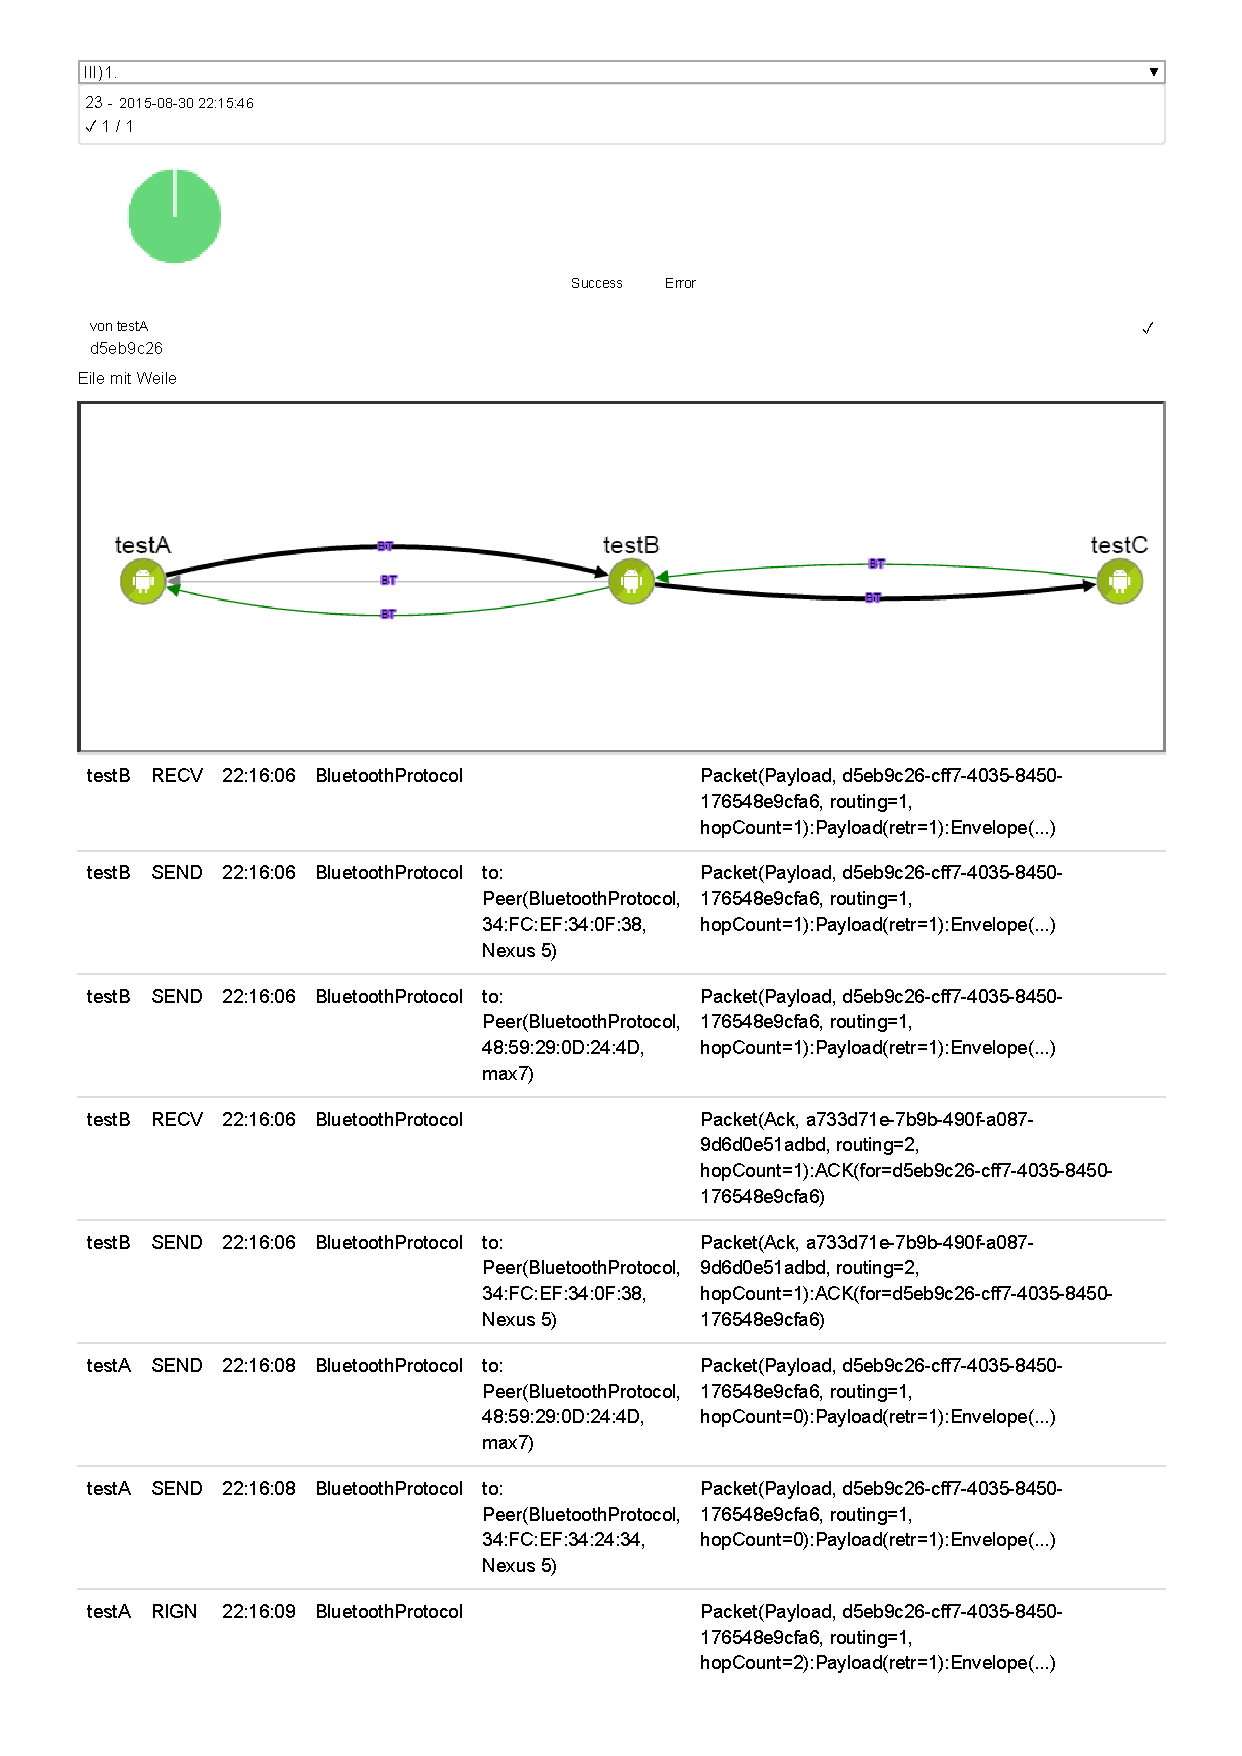
\includegraphics[trim=0 100 0 0,clip,scale=0.8]{belege/manuelle-tests/netzwerk/Dashboardauszuege/Netzwerktest_III-1.pdf}
\clearpage

\paragraph{Test N-iii-2 Bluetooth-Wegfindung zum nächsten Knoten mit Internetverbindung}

Der Test war erfolgreich.

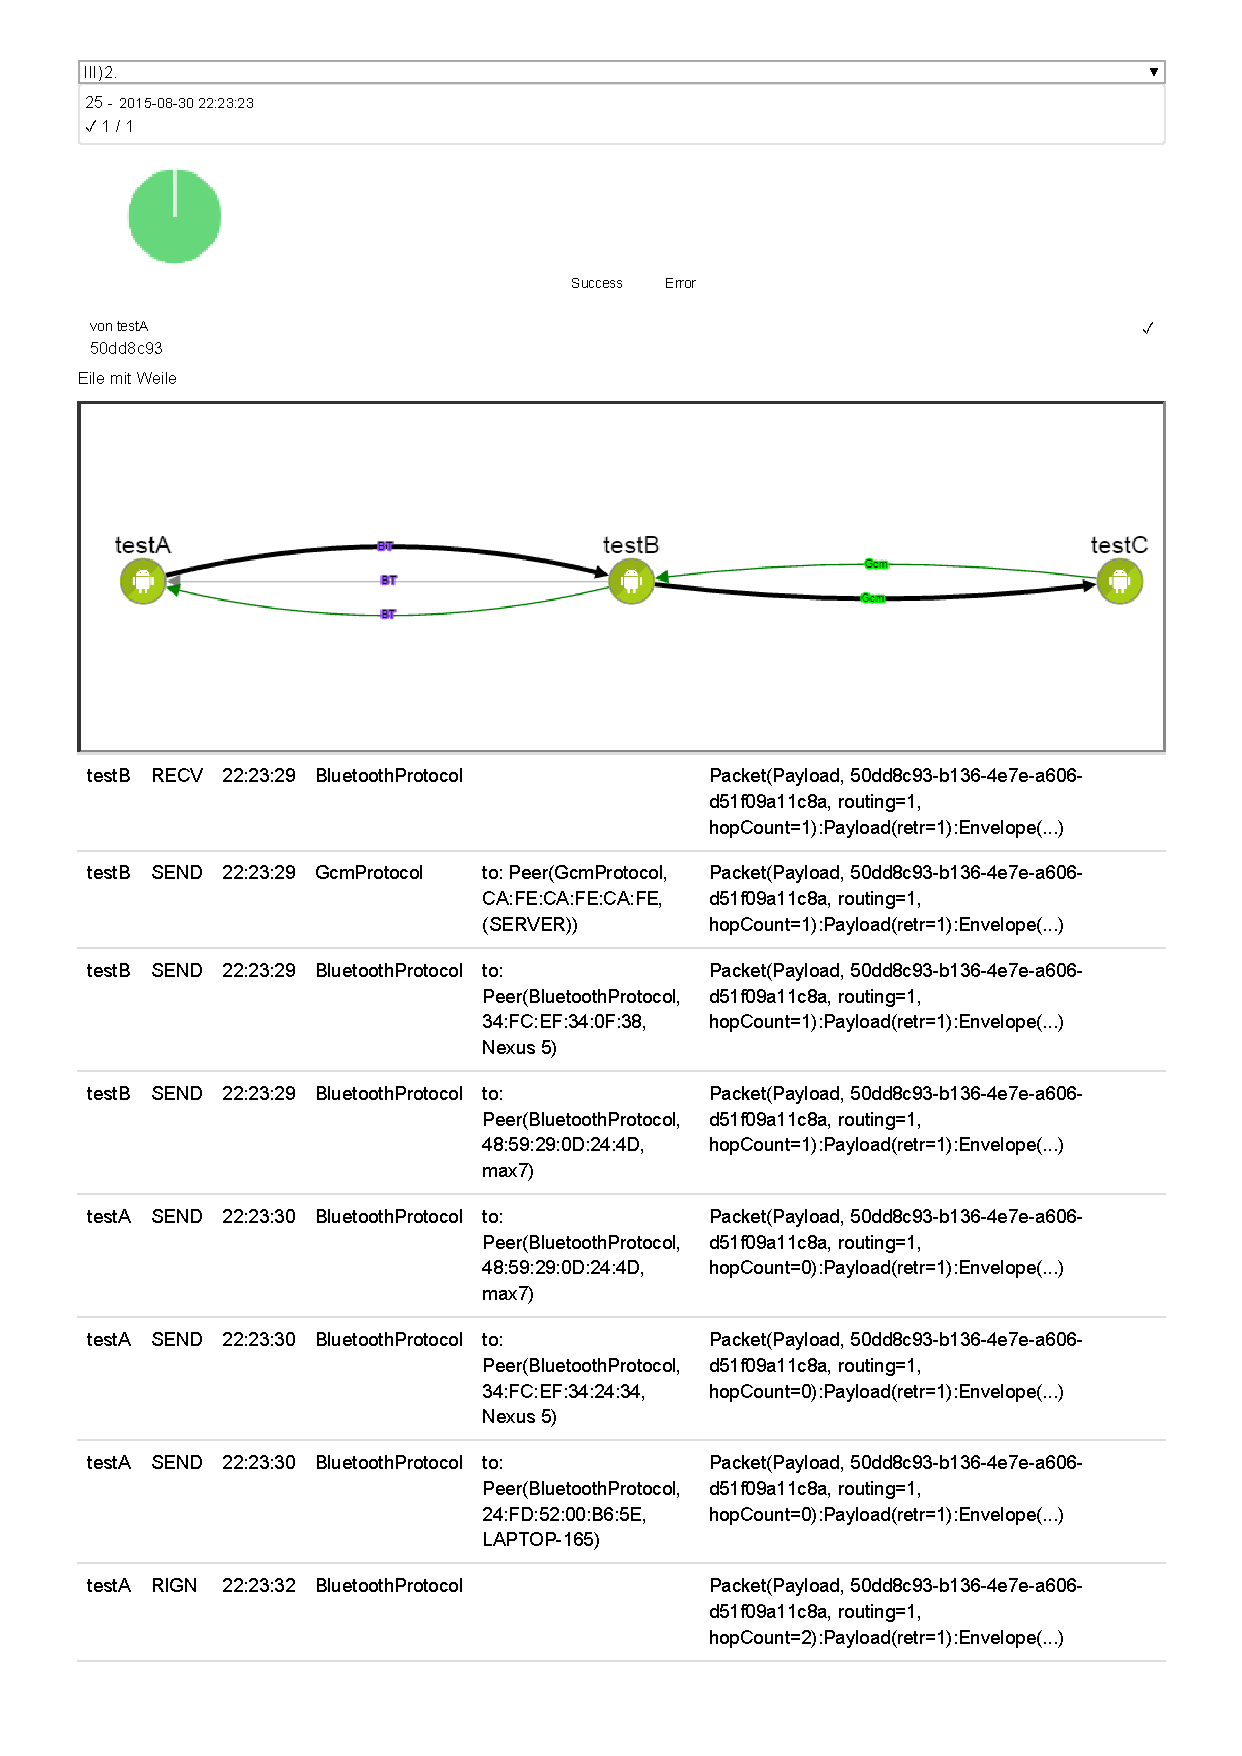
\includegraphics[trim=0 120 0 0,clip,scale=0.8]{belege/manuelle-tests/netzwerk/Dashboardauszuege/Netzwerktest_III-2.pdf}
\clearpage


\paragraph{Teil N-iv Testfälle für sich verändernde Routen}

\paragraph{Test N-iv.1 \glqq Abreißende\grqq~ Bluetooth-Verbindung}

Der Test war erfolgreich.

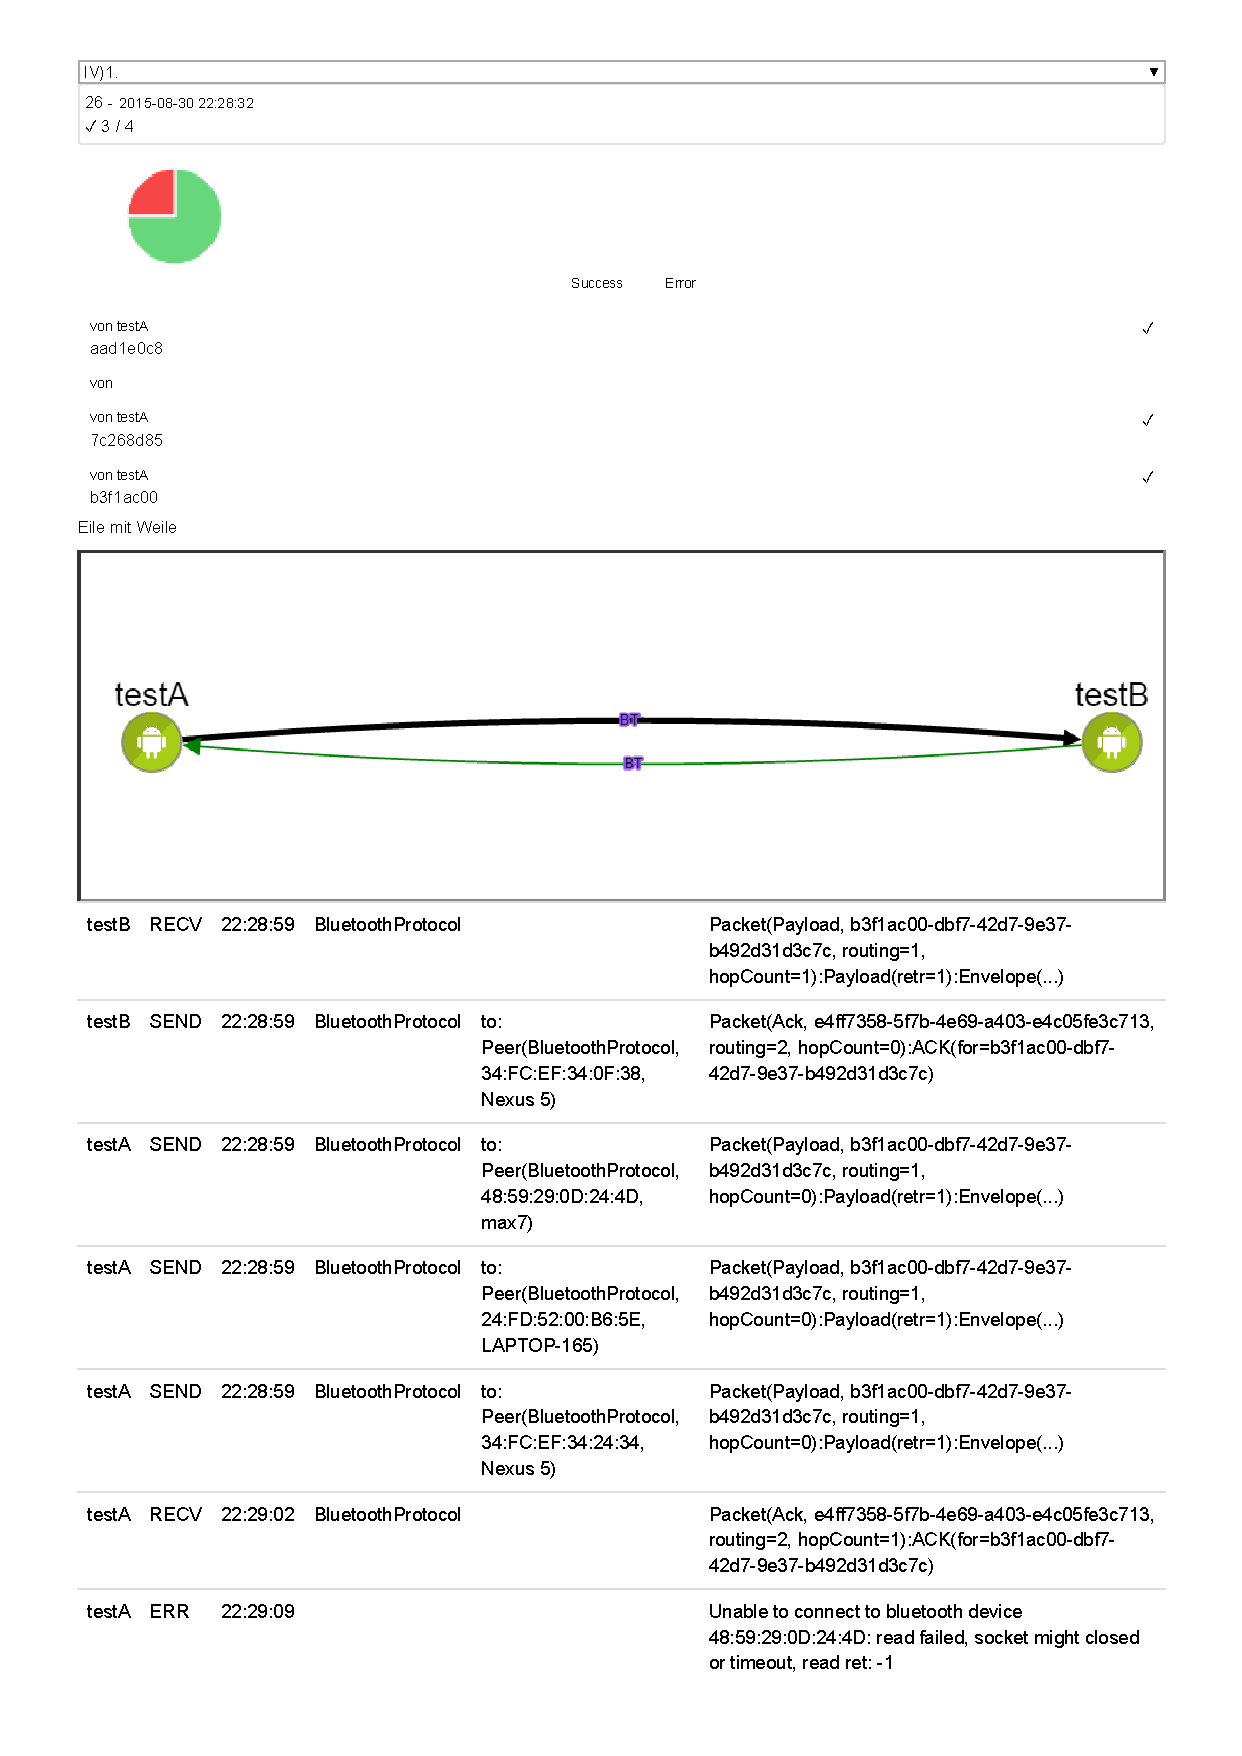
\includegraphics[trim=0 120 0 0,clip,scale=0.8]{belege/manuelle-tests/netzwerk/Dashboardauszuege/Netzwerktest_IV-1a.pdf}
\clearpage
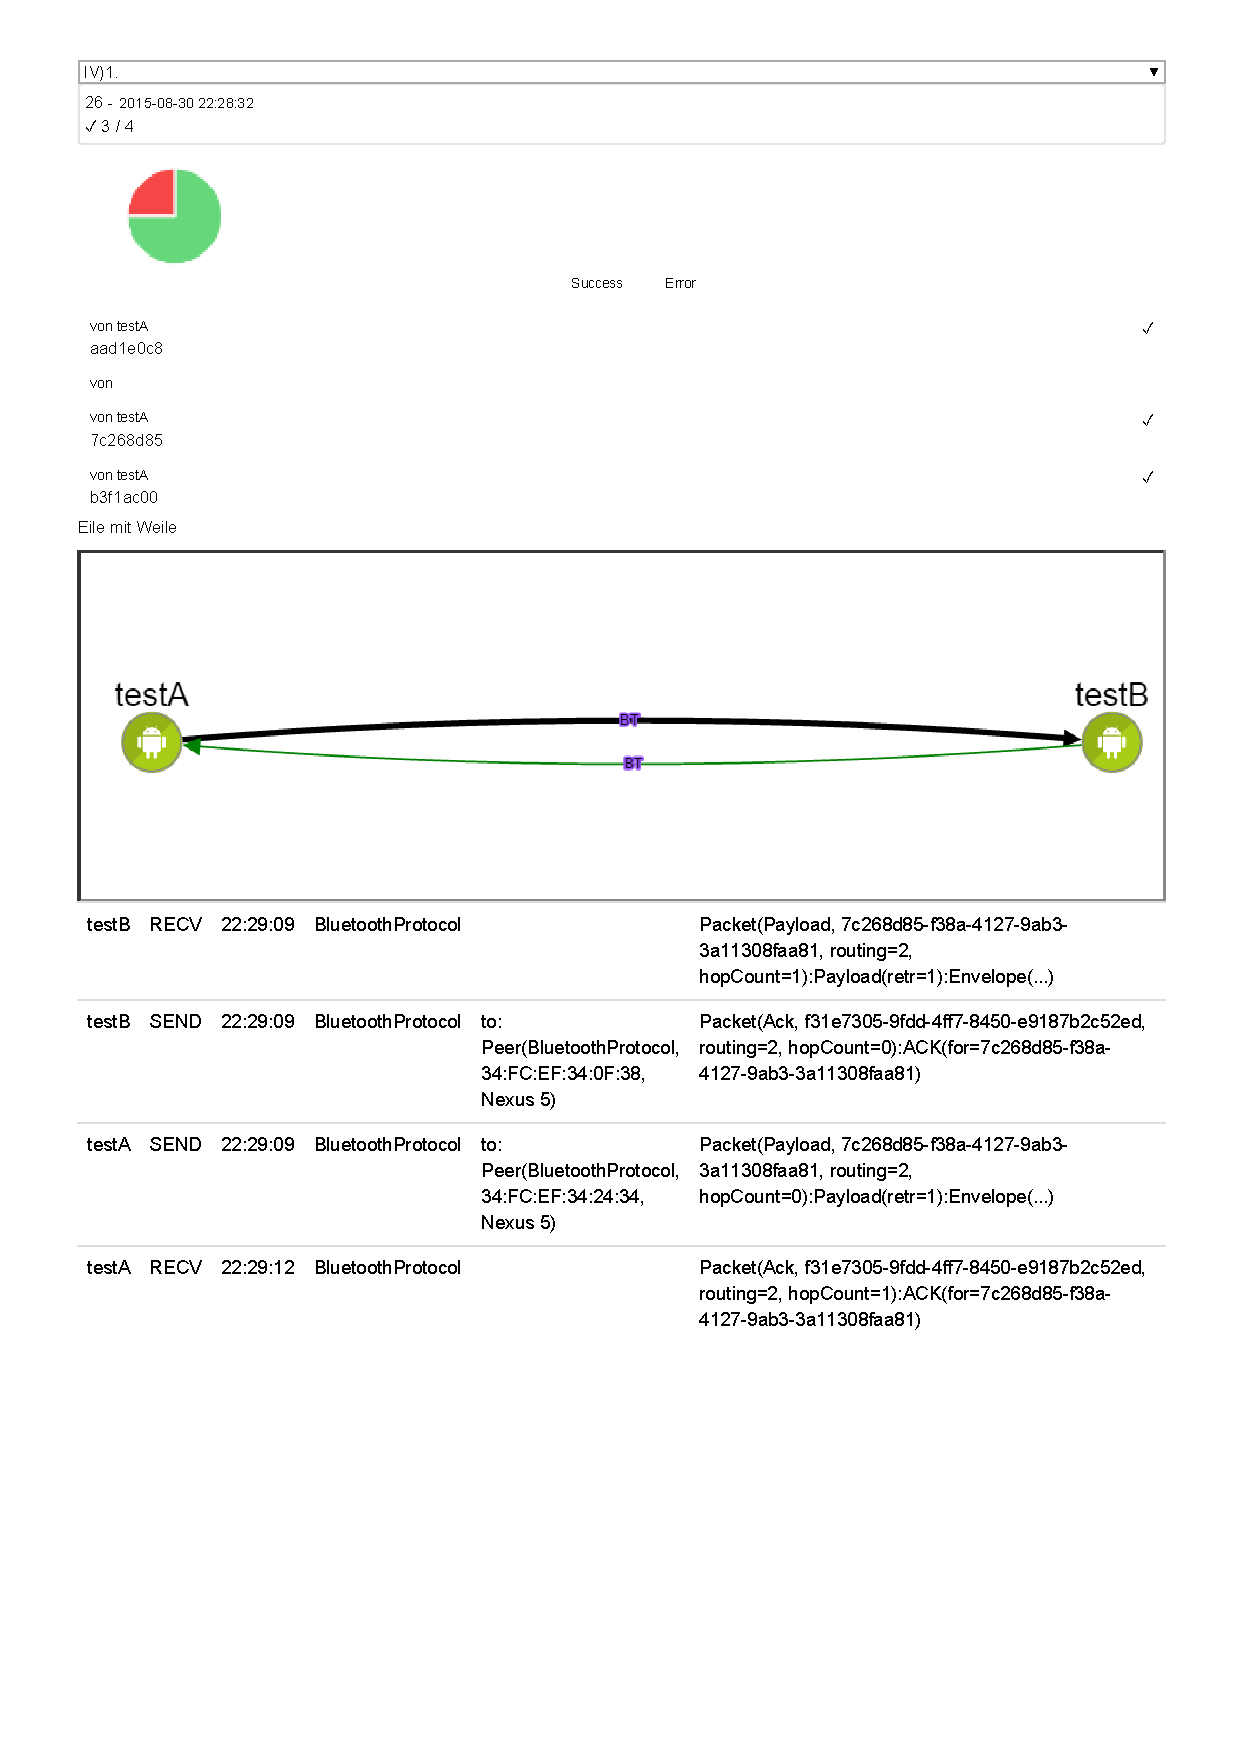
\includegraphics[trim=0 90 0 0,clip,scale=0.8]{belege/manuelle-tests/netzwerk/Dashboardauszuege/Netzwerktest_IV-1b.pdf}
\clearpage
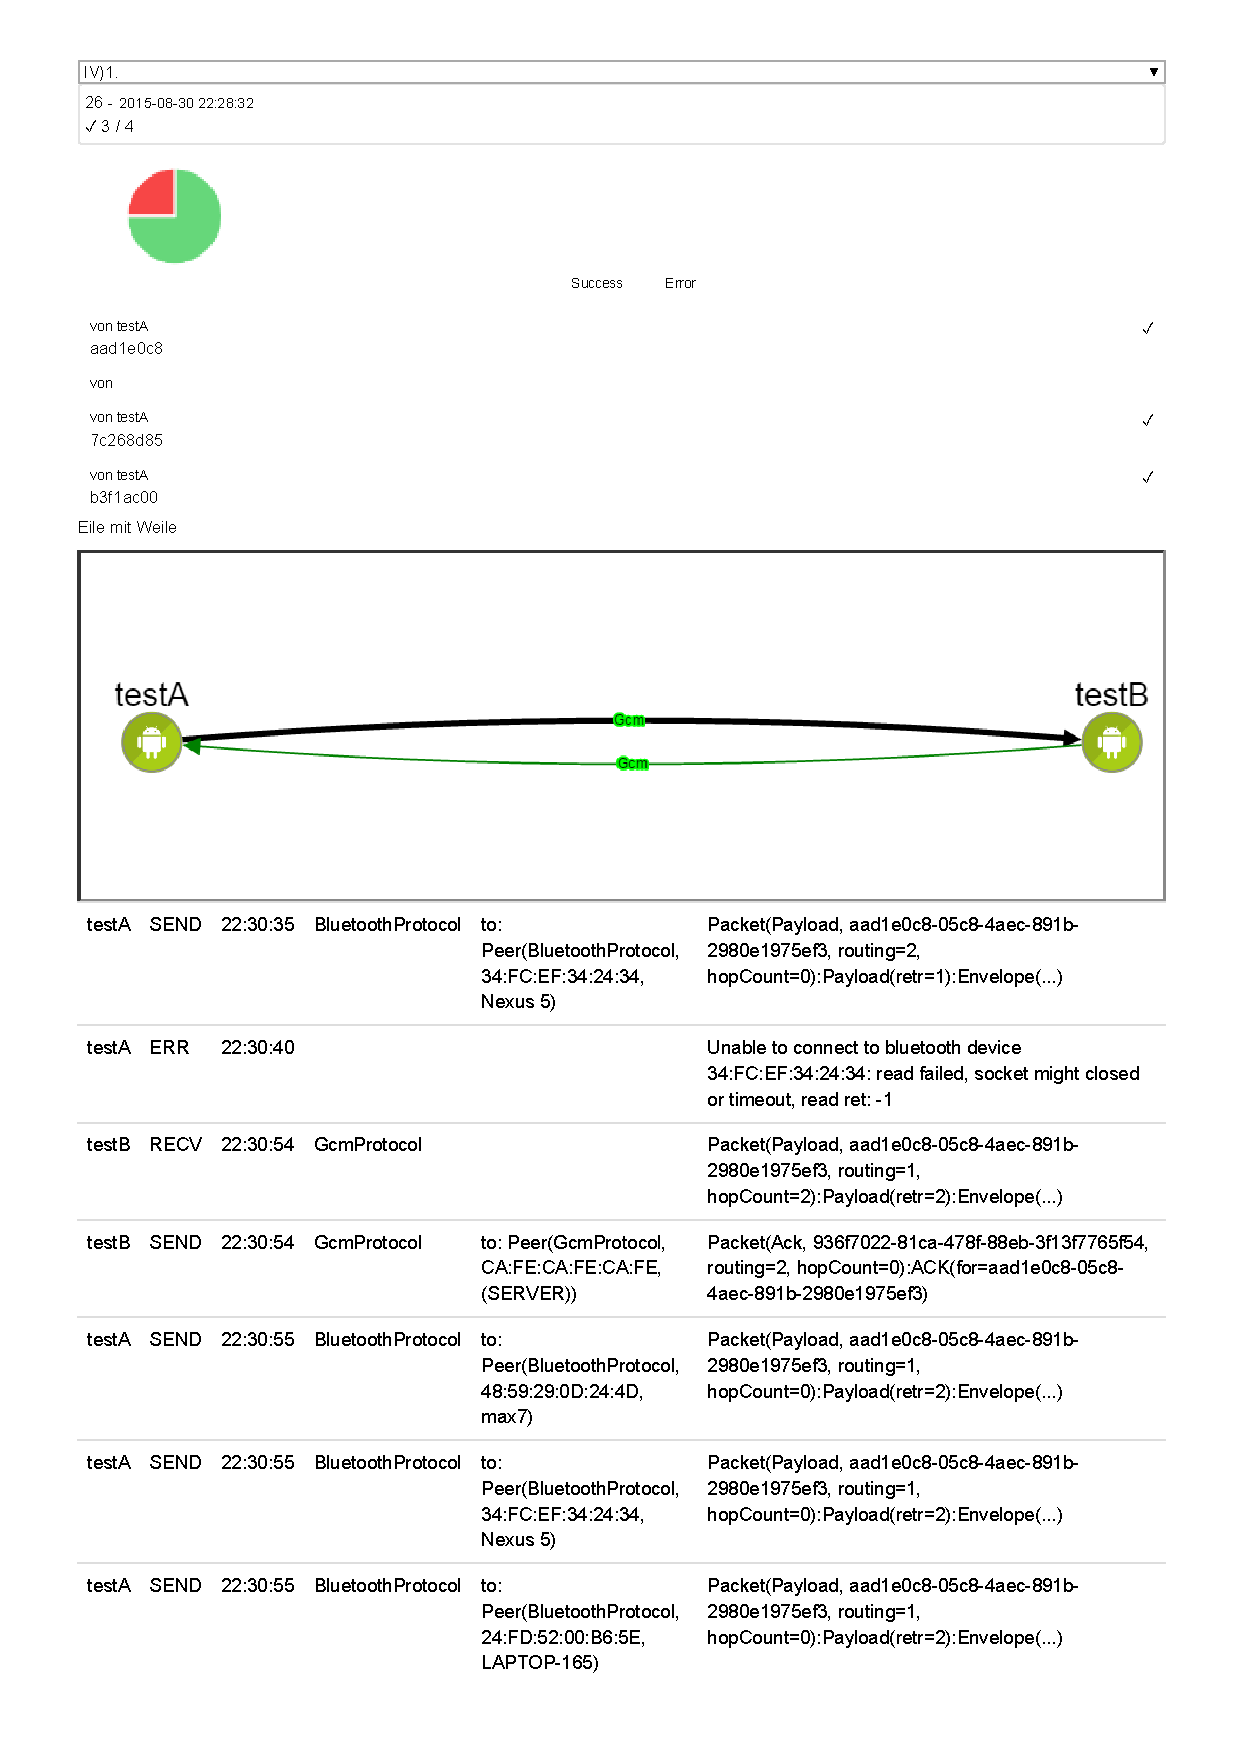
\includegraphics[trim=0 30 0 0,clip,scale=0.8]{belege/manuelle-tests/netzwerk/Dashboardauszuege/Netzwerktest_IV-1c.pdf}
\clearpage



\clearpage

\subsection{Durchführung des manuellen Netzwerk-Testplans vom 13. September 2015}

\textbf{Durchgeführt von:} Matthias Hofmann

\textbf{Änderungen vorgenommen in Commit:} keine Änderungen nötig

\paragraph{Teil N-ii Testfälle für die allgemeine Übertragung}

\paragraph{Test N-ii.1 Test der direkten Übertragung via Flooding / Bluetooth}

Der Test war erfolgreich.

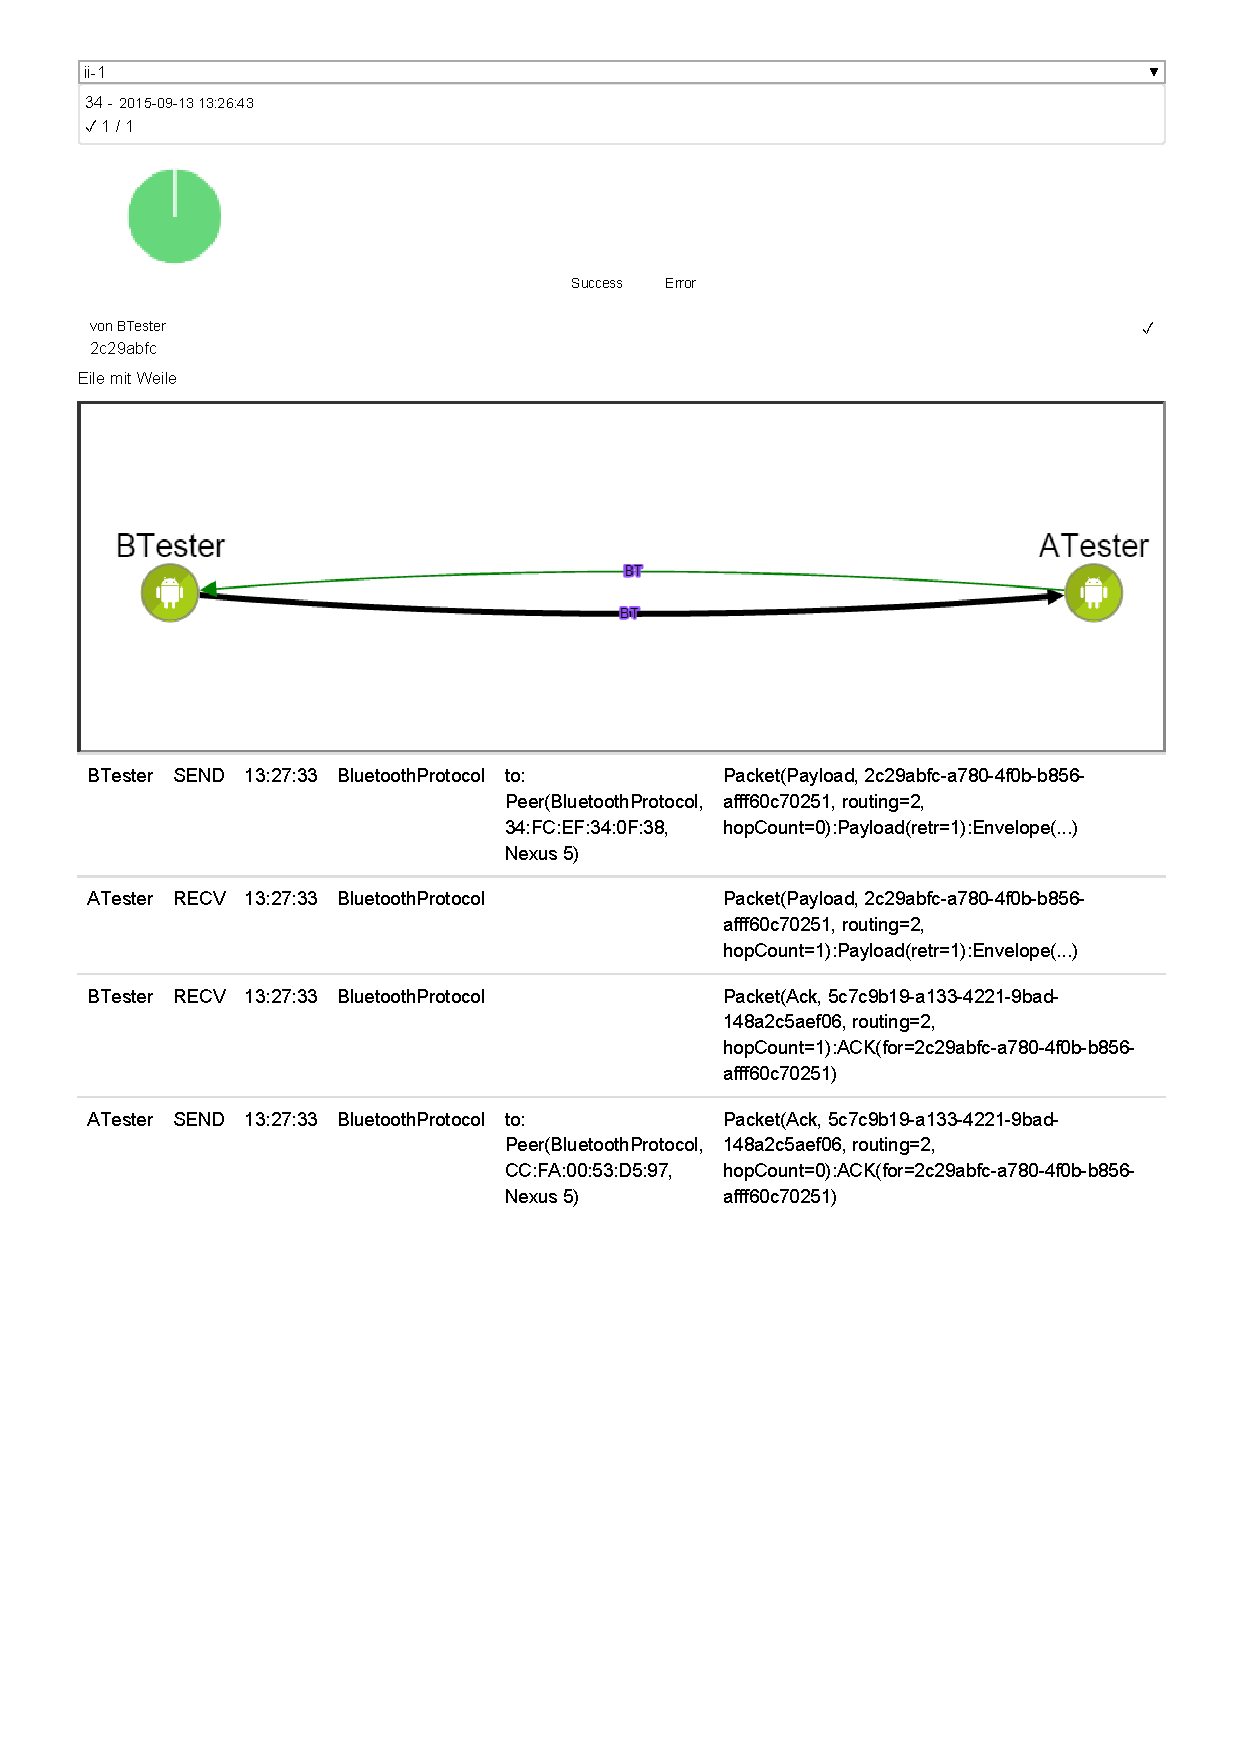
\includepdf[offset=-0.8cm 0,scale=.8,pagecommand={}]{belege/manuelle-tests/netzwerk/Dashboardauszuege/Netzwerktest_n-ii-1.pdf}

\paragraph{Test N-ii.2 Test der direkten Übertragung via DSR / Bluetooth}

Der Test war erfolgreich.

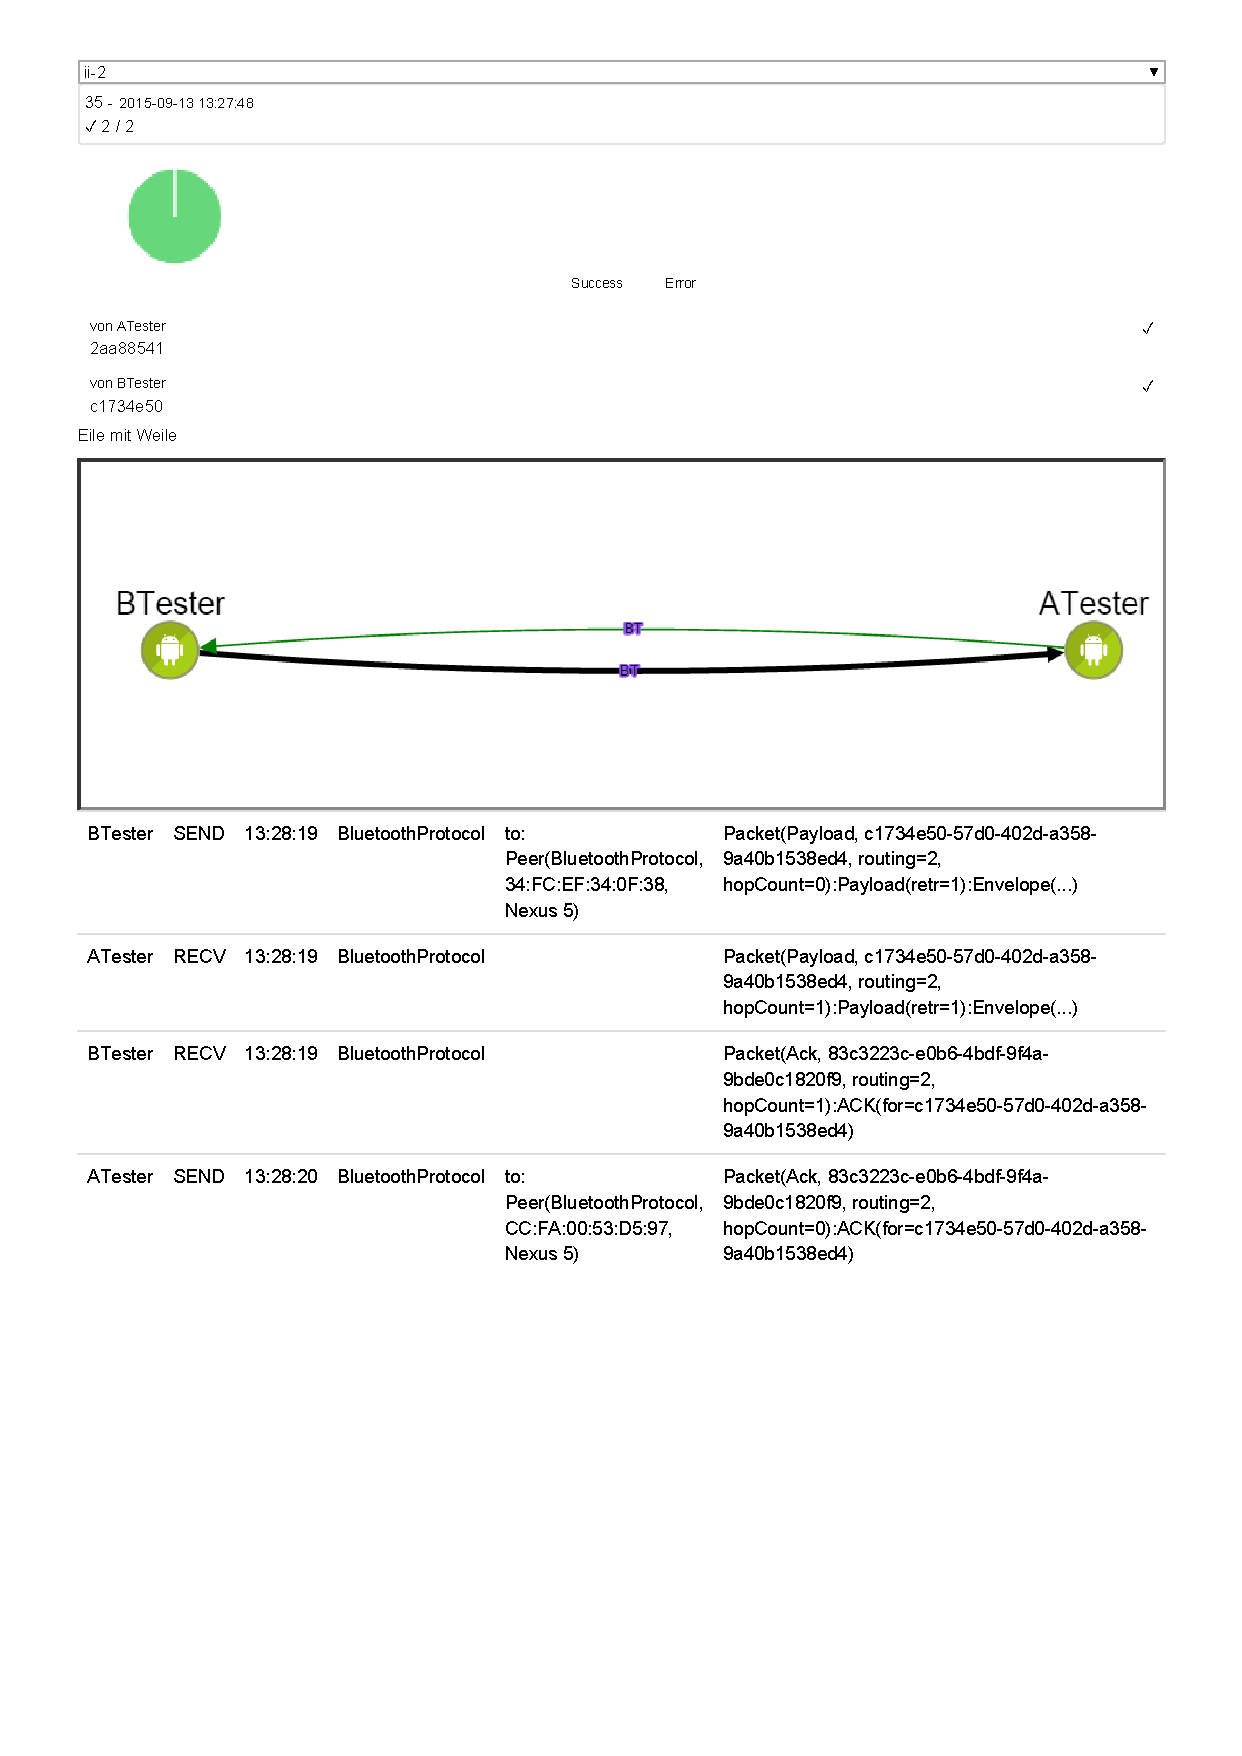
\includepdf[offset=-0.8cm 0,scale=.8,pagecommand={}]{belege/manuelle-tests/netzwerk/Dashboardauszuege/Netzwerktest_n-ii-2a.pdf}
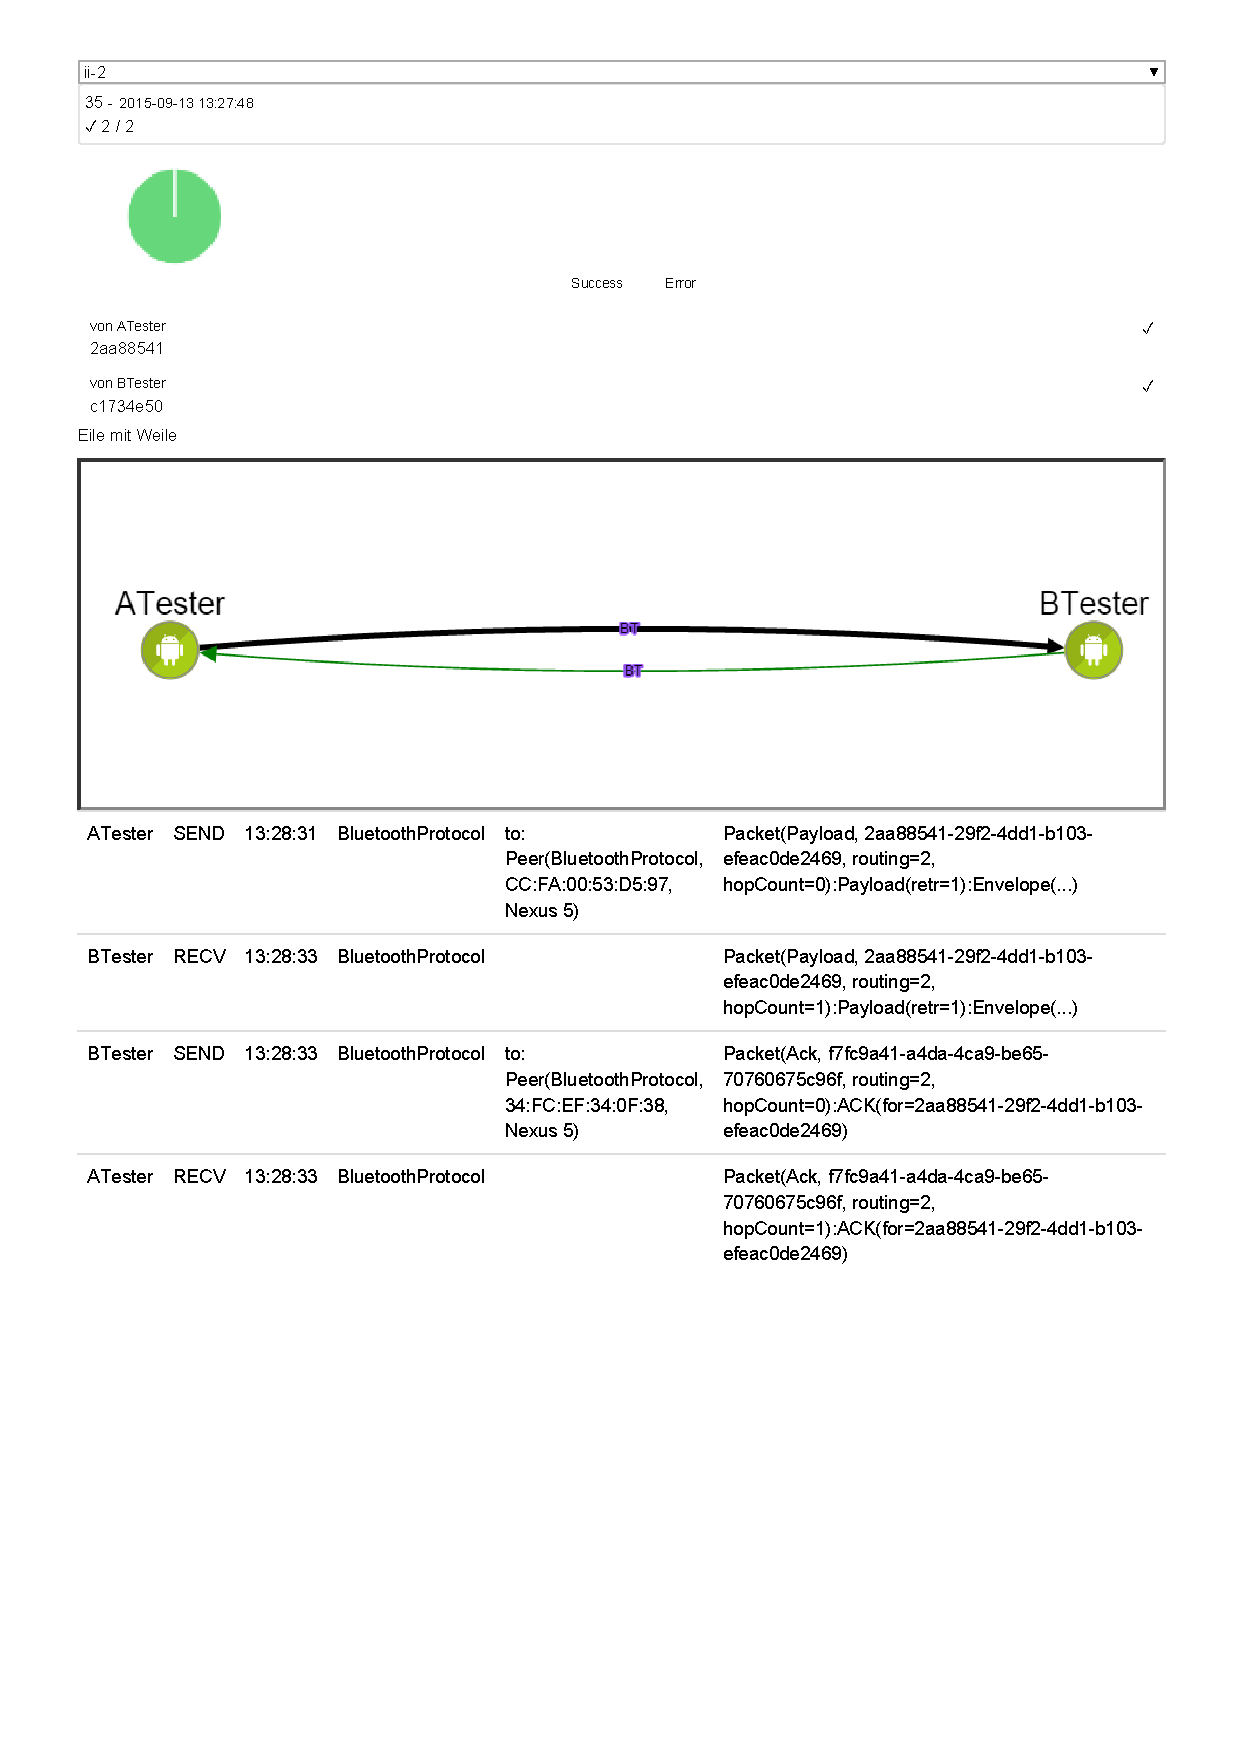
\includepdf[offset=-0.8cm 0,scale=.8,pagecommand={}]{belege/manuelle-tests/netzwerk/Dashboardauszuege/Netzwerktest_n-ii-2b.pdf}

\paragraph{Test N-ii.3 Test der direkten Übertragung via Server / Google Cloud Messaging}

Der Test war erfolgreich.

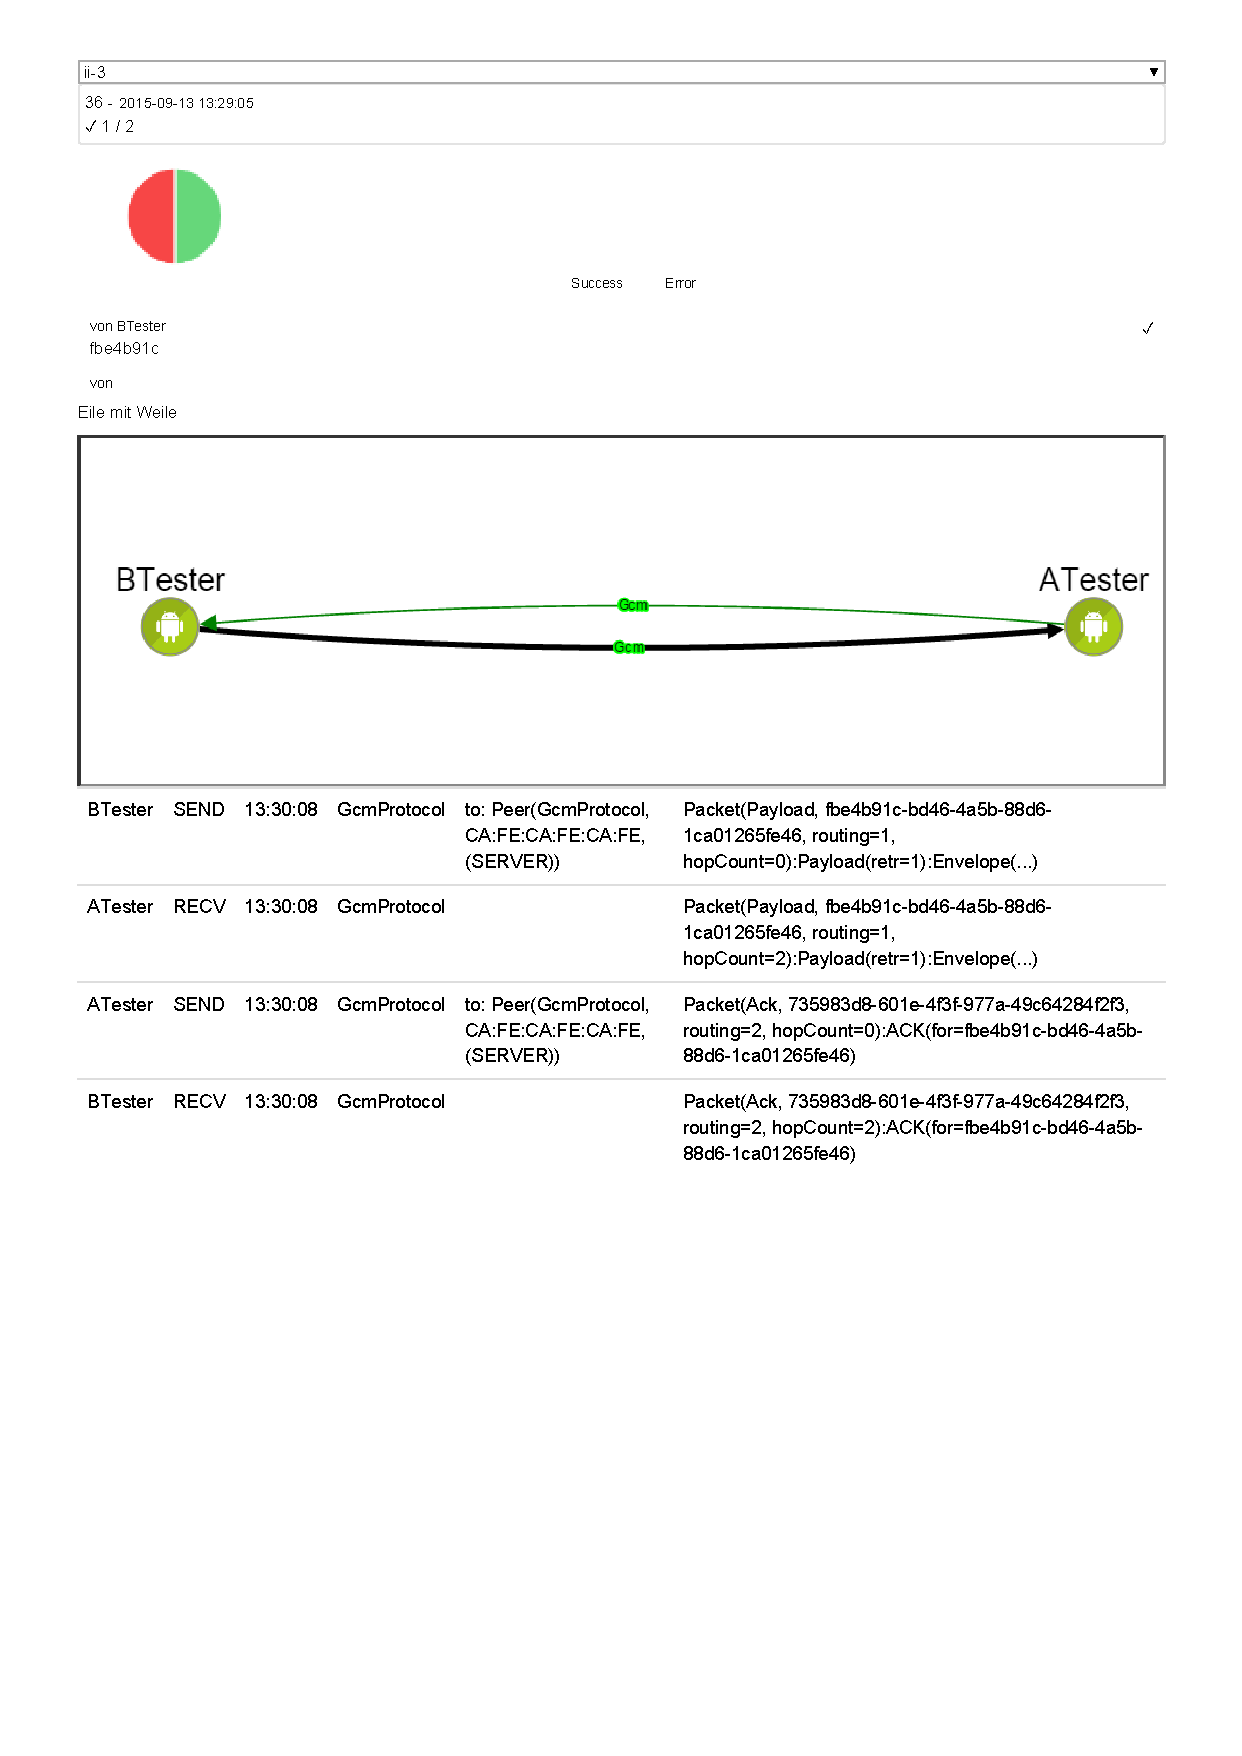
\includepdf[offset=-0.8cm 0,scale=.8,pagecommand={}]{belege/manuelle-tests/netzwerk/Dashboardauszuege/Netzwerktest_n-ii-3.pdf}


\paragraph{Teil N-iii Testfälle für Wegfindung per Flooding und einfaches Routing}

\paragraph{Test N-iii.1 Bluetooth-Wegfindung - Flooding mit drei Knoten}

Der Test war erfolgreich.

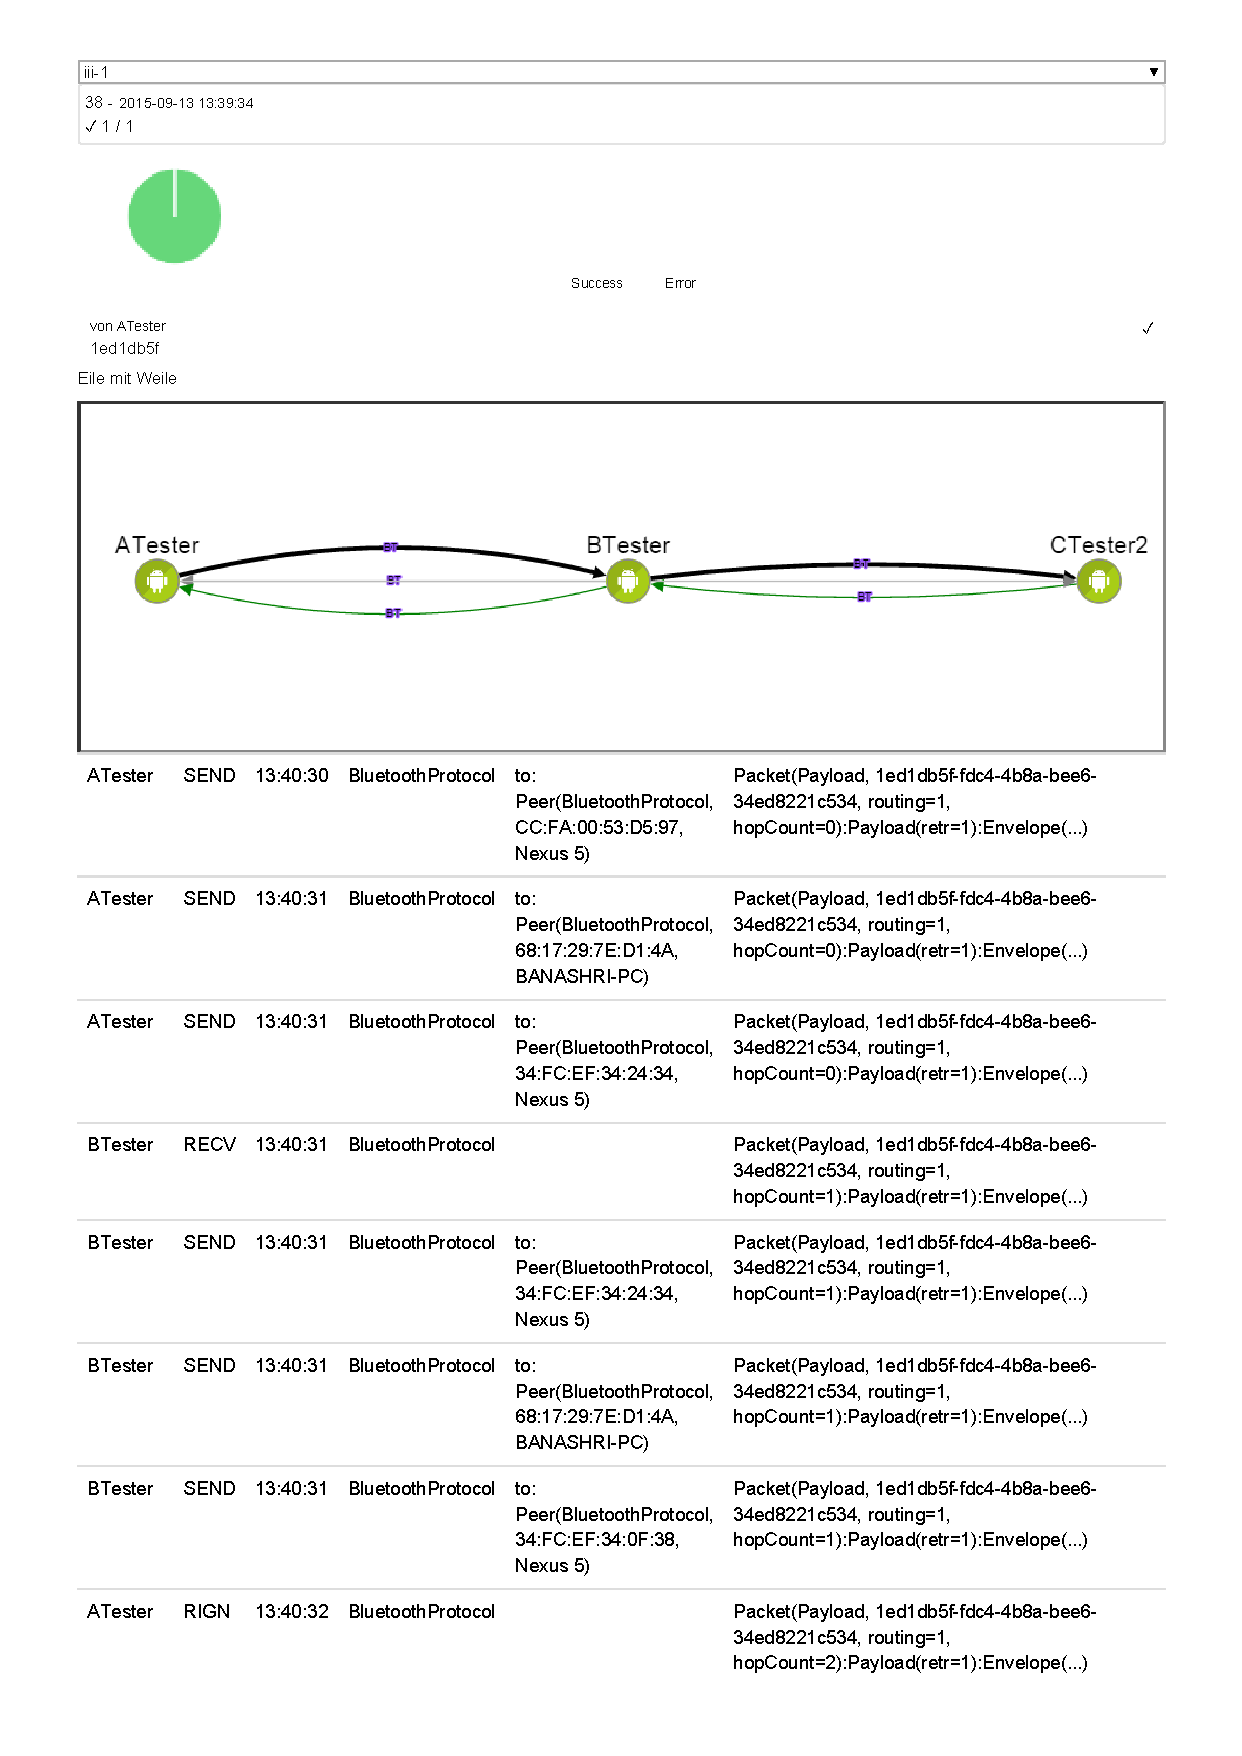
\includepdf[offset=-0.8cm 0,scale=.8,pagecommand={}]{belege/manuelle-tests/netzwerk/Dashboardauszuege/Netzwerktest_n-iii-1.pdf}

\paragraph{Test N-iii-2 Bluetooth-Wegfindung zum nächsten Knoten mit Internetverbindung}

Der Test war erfolgreich.

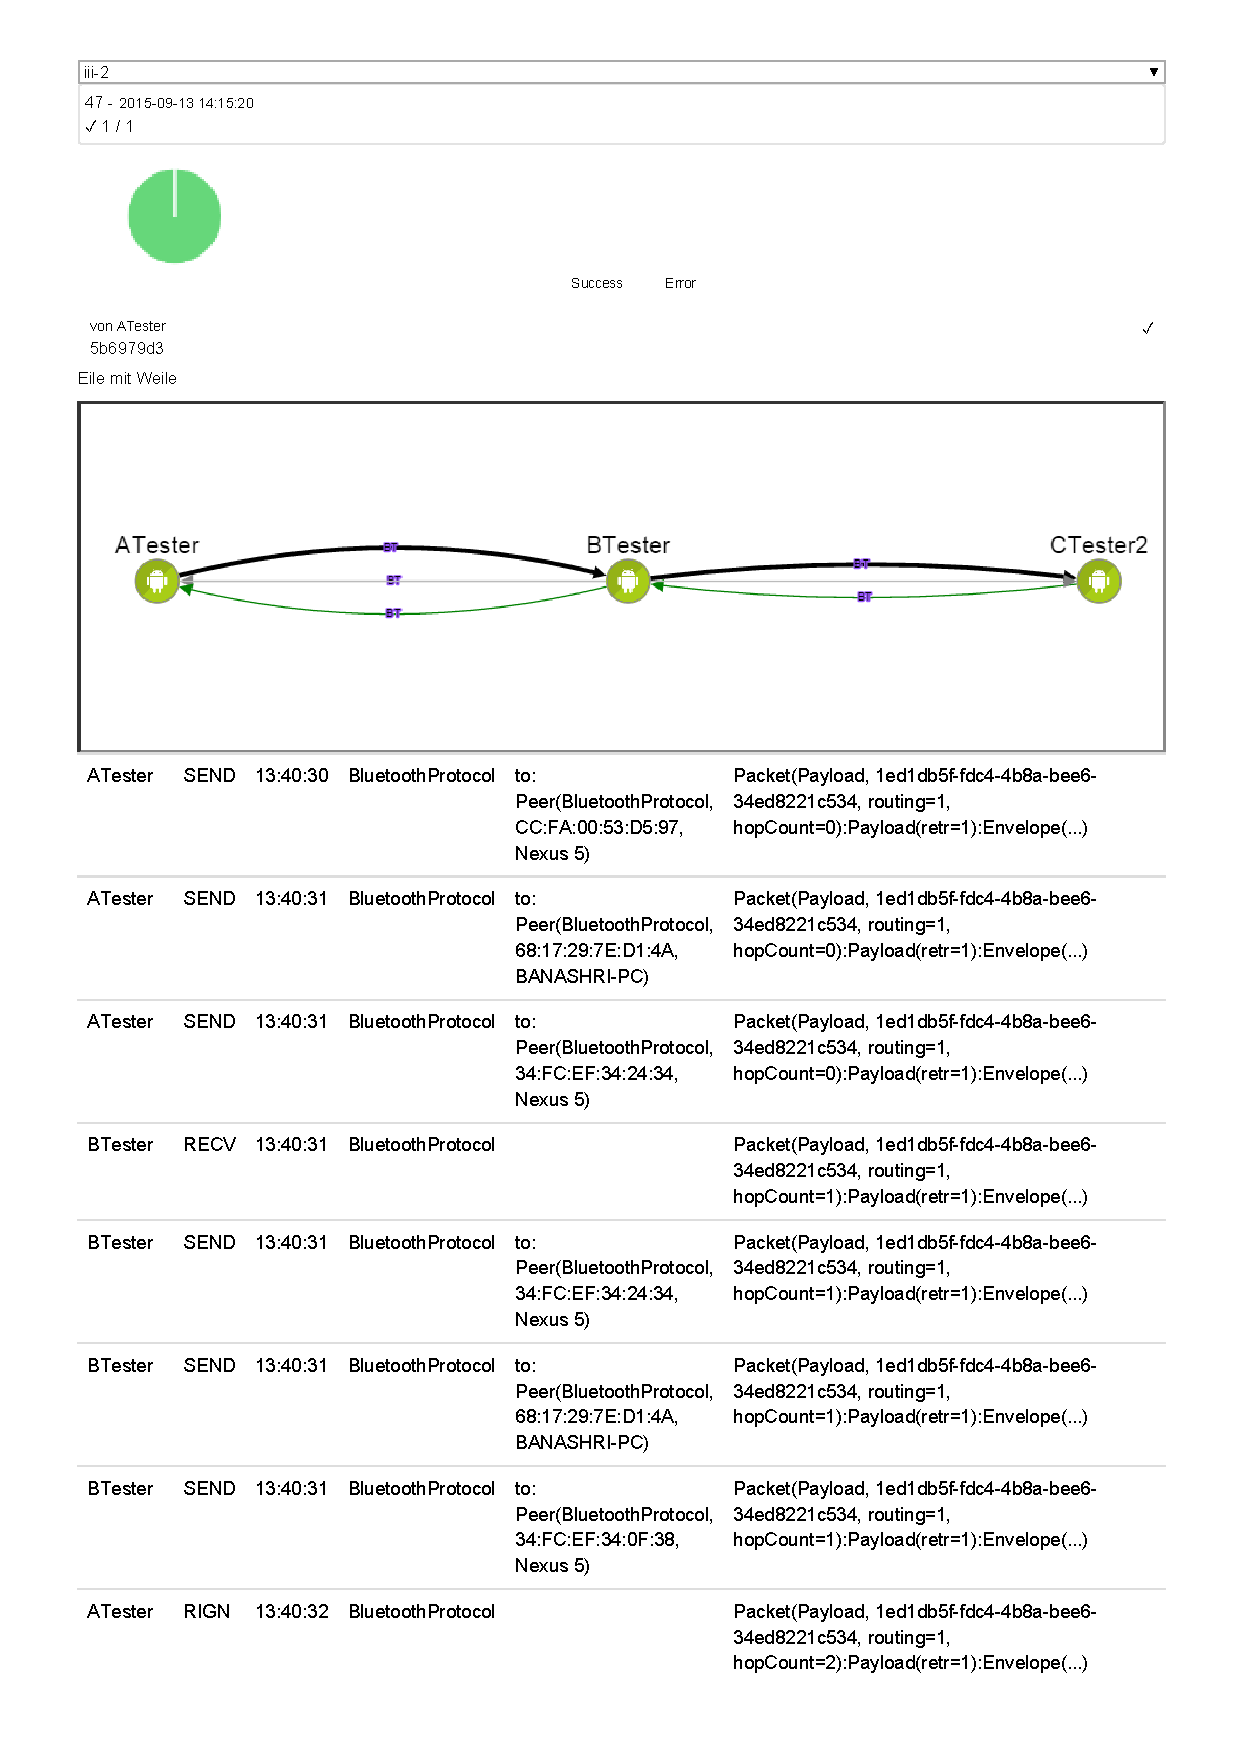
\includepdf[offset=-0.8cm 0,scale=.8,pagecommand={}]{belege/manuelle-tests/netzwerk/Dashboardauszuege/Netzwerktest_n-iii-2.pdf}


\paragraph{Teil N-iv Testfälle für sich verändernde Routen}

\paragraph{Test N-iv.1 \glqq Abreißende\grqq~ Bluetooth-Verbindung}

Der Test war erfolgreich.

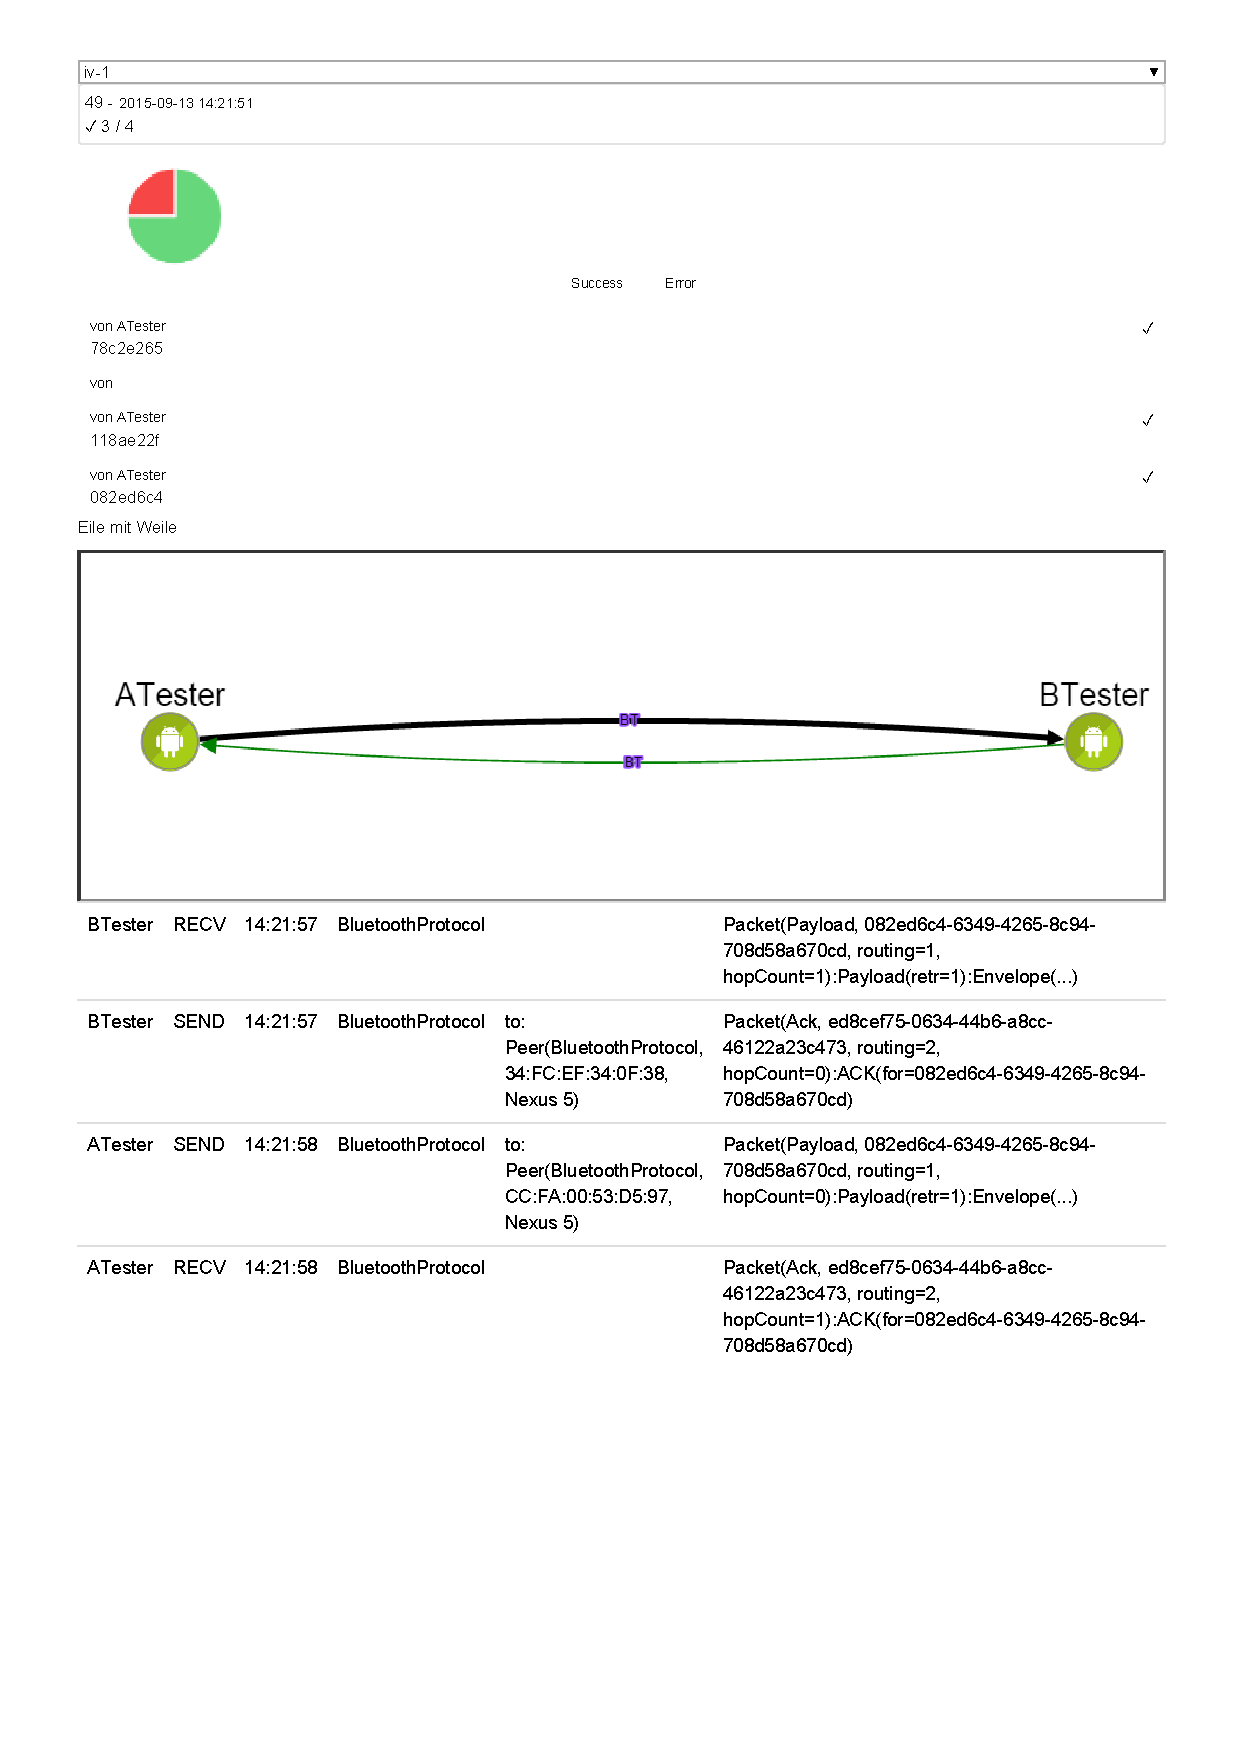
\includepdf[offset=-0.8cm 0,scale=.8,pagecommand={}]{belege/manuelle-tests/netzwerk/Dashboardauszuege/Netzwerktest_n-iv-1a.pdf}
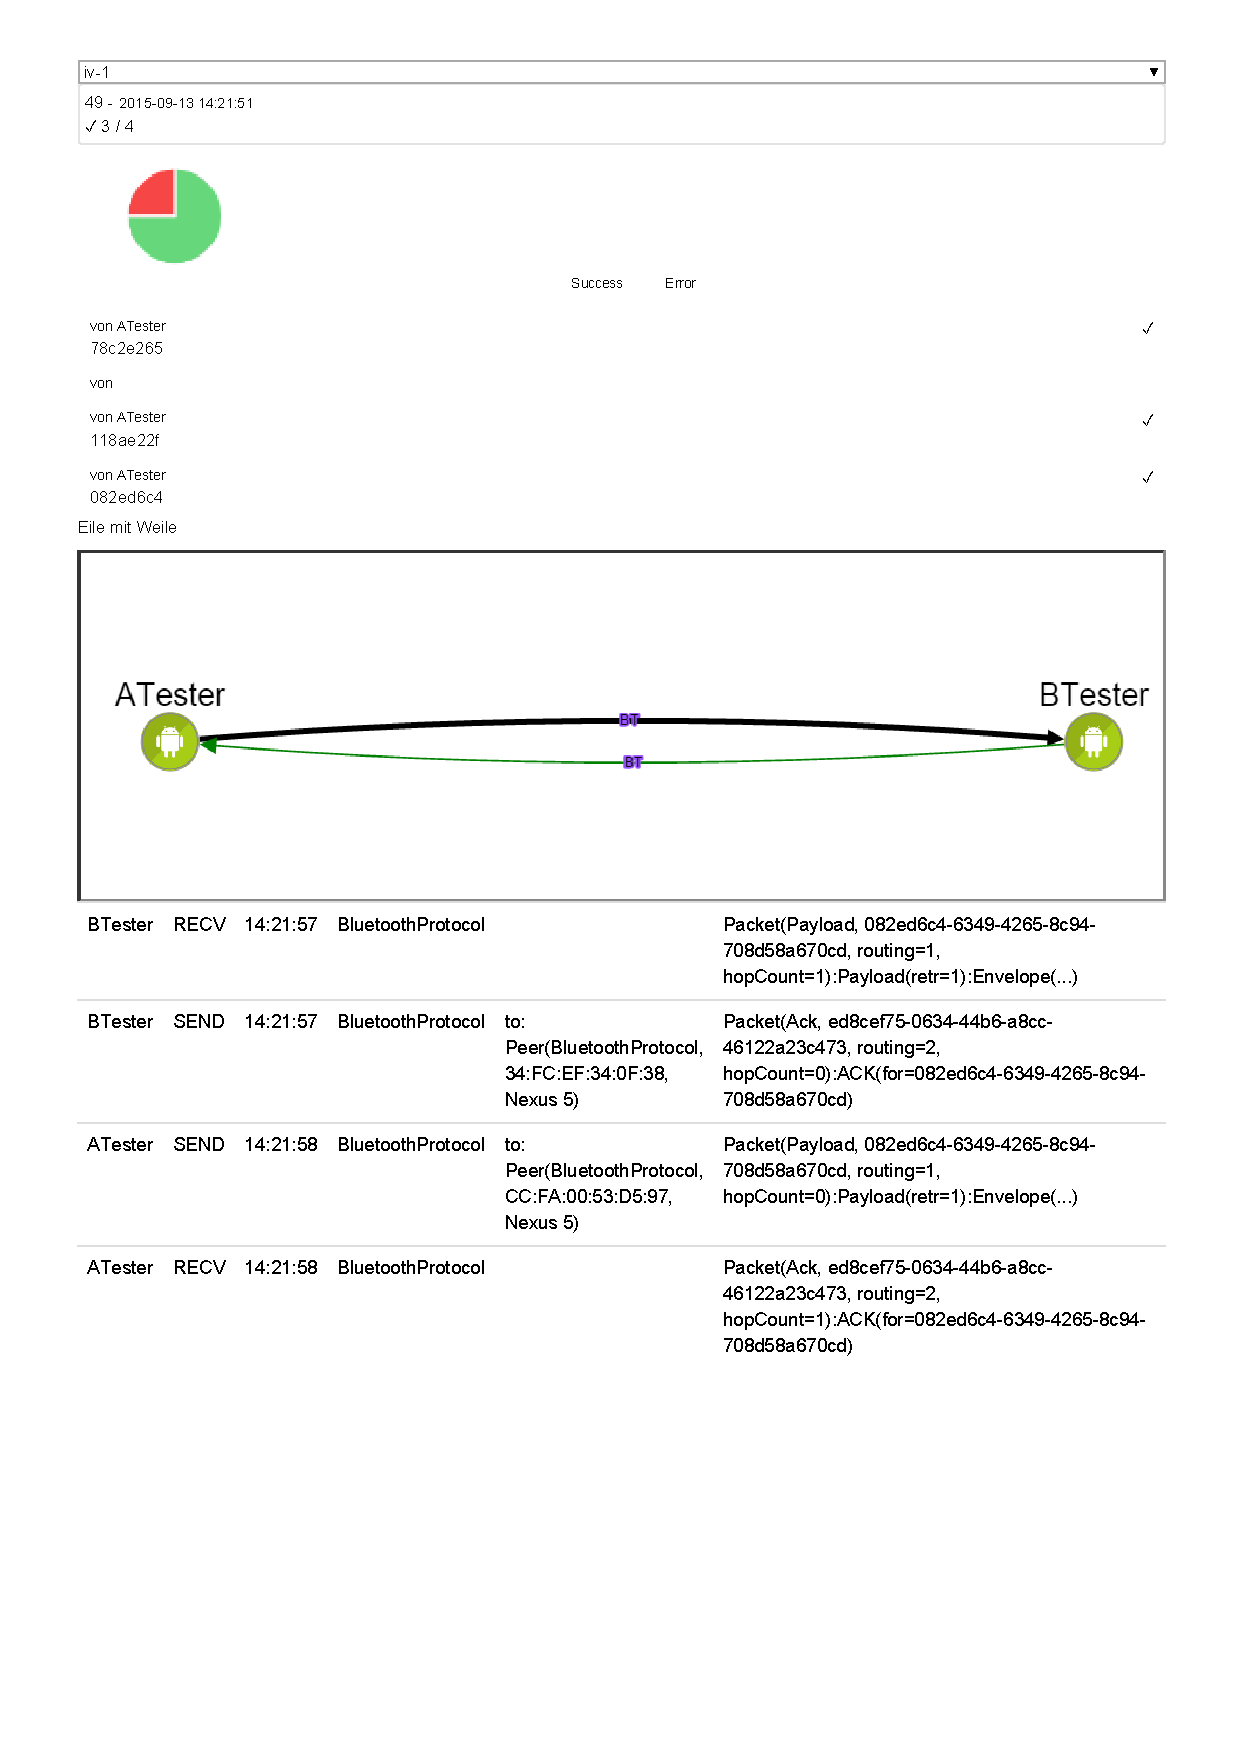
\includepdf[offset=-0.8cm 0,scale=.8,pagecommand={}]{belege/manuelle-tests/netzwerk/Dashboardauszuege/Netzwerktest_n-iv-1b.pdf}
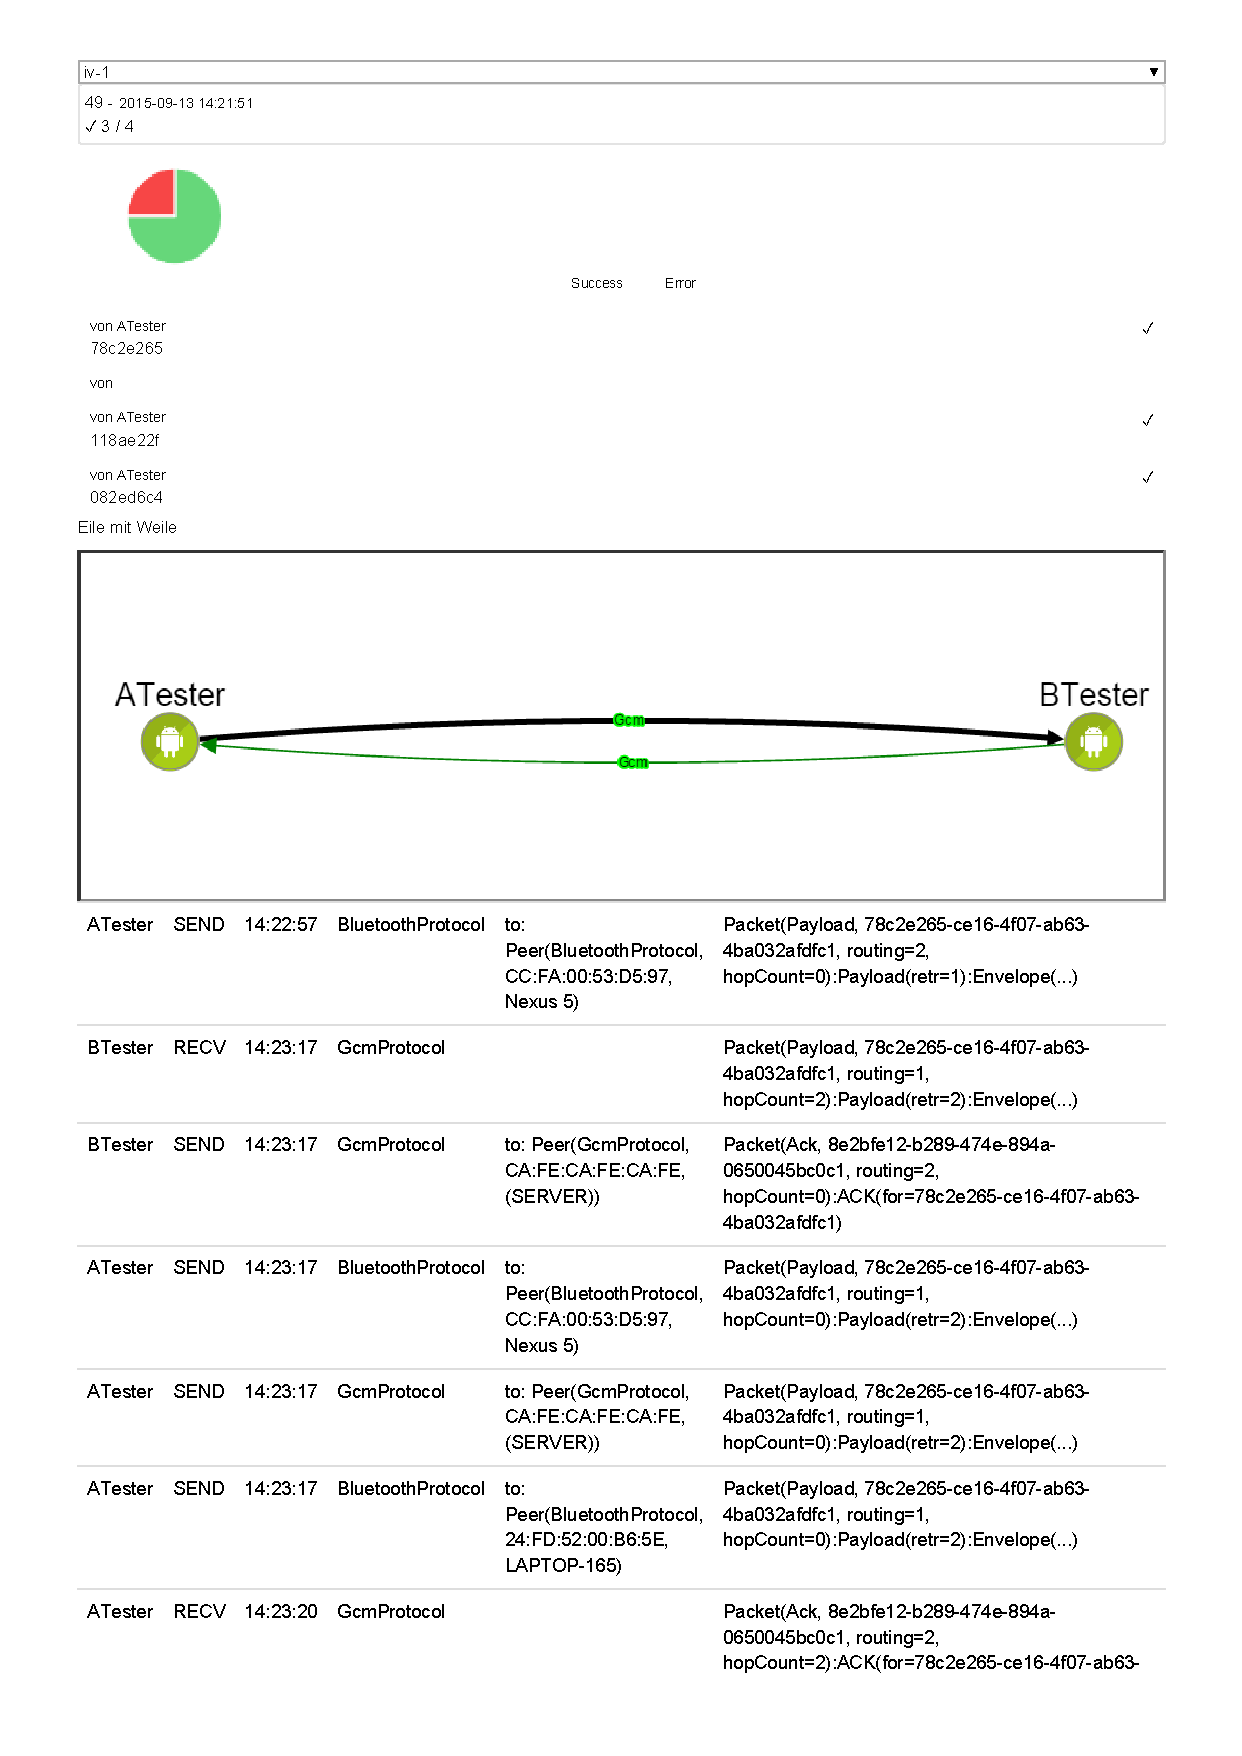
\includepdf[offset=-0.8cm 0,scale=.8,pagecommand={}]{belege/manuelle-tests/netzwerk/Dashboardauszuege/Netzwerktest_n-iv-1c.pdf}



\clearpage

\section{Großtests}

Um das Verhalten der App bei einem tatsächlichen Einsatz mit vielen Benutzern und vielen Geräten zu simulieren, haben wir Großtests nach dem folgenden Testplan durchgeführt.

\subsubsection{Allgemeine Ausgangskonfiguration der Knoten:}\label{Ausgangskonfiguration}

Ein Knoten ist, soweit nicht näher beschrieben, ein Android-Gerät, auf dem die aktuellste Version der App eingerichtet und die initiale Einrichtung (Eingabe eines Nicknames, dadurch Registrierung des Gerätes mit Nickname, GCM-ID und PublicKey am Server) abgeschlossen ist.

\subsubsection{Eigenschaften:}\label{Eigenschaften}

\begin{itemize}
\tightlist
\item
Geringe Distanz: Die Knoten stehen nahe zu ihren Nachbarn (1m).
\item
Mittlere Distanz: Die Knoten stehen etwas entfernt zu ihren Nachbarn (5m).
\item
Große Distanz: Die Knoten stehen weit entfernt zu ihren Nachbarn (10m).
\end{itemize}

\subsubsection{Testfälle für Statistik Erhebungen}\label{Testfaelle}

\paragraph*{Testaufbau:}
Wir führen einen Test mit 10 Handys durch. Es wird nur Bluetooth getestet. Alle Handys haben dauerhaft Verbindung in das Internet um ständige Nachrichtenverläufe an unser Dashboard zu senden, damit wir den Test auswerten können. Die Handys werden Kugelförmig positioniert und
während des Tests nicht bewegt. Es werden viele Nachrichten verschickt. (Ca. eine Nachricht alle 2 Sekunden) Die Handys können jedoch keine Nachrichten über das Internet versenden. Dies wird in der App abgestellt. Die Nachrichten wurden alle per Hand verschickt. Kleine Abweichungen bei Distanz oder Sendegeschwindigkeit werden hingenommen. Jeder Test läuft 5 Minuten. 
\paragraph*{Test 1:}
Die einzelnen Handys haben eine geringe Distanz zueinander. 
\paragraph*{Test 2:}
Die einzelnen Handys haben eine mittlere Distanz zueinander. 
\paragraph*{Test 3:}
Die einzelnen Handys haben eine große Distanz zueinander. 

\clearpage

\subsection{Durchführung des Großtests 1}

Der Test wurde 31.08.2015 durchgeführt. Eine Durchführung zu einem früheren Zeitpunkt war nicht möglich, da erst in Sprint 8 das Routing implementiert wurde.
Die Handys wurden mit Buchstaben benannt und in Raum C205 verteilt.


\subsubsection{Ergebnisse Test 1}

Wir haben auf 117 Nachrichten 11 erfolgreiche Fälle und 106 Errors.

\paragraph{Folgende Beispiele veranschaulichen Nachrichten, die beim Empfänger angekommen sind:}

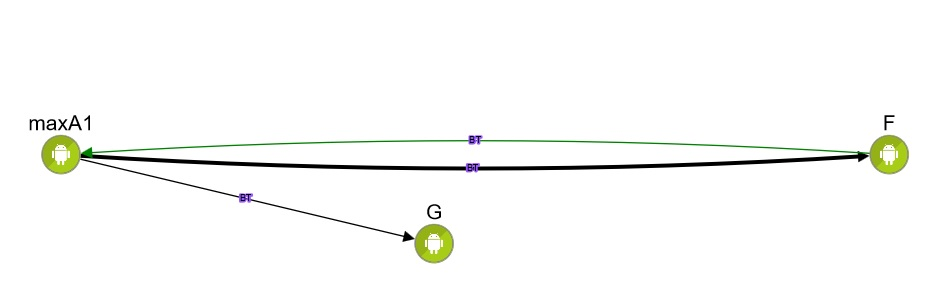
\includegraphics[width=1.0\textwidth]{belege/grosstests/Bilder/Erfolg4.jpg}\\
1. A sendet eine Nachricht an F. A sendet die Nachricht an G und F los, da A nur den
Bluetooth Namen der Handys kennt, und so nicht weiß, dass F sich in
Reichweite befindet. F sendet ein Acknowledgement zurück, während G die
Nachricht nicht weiterleiten kann.\\
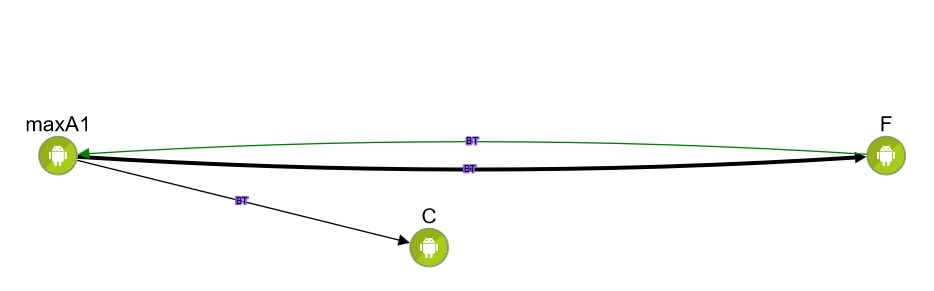
\includegraphics[width=1.0\textwidth]{belege/grosstests/Bilder/Erfolg3.jpg}\\
2. Gleiches Szenario wie in 1, nur diesmal mit C statt G.\\
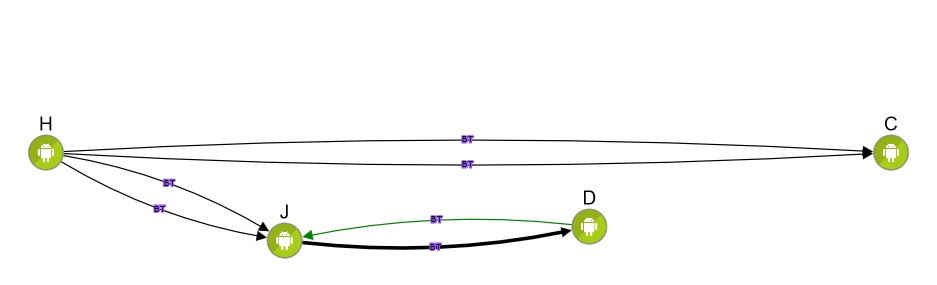
\includegraphics[width=1.0\textwidth]{belege/grosstests/Bilder/Erfolg2.jpg}\\ 3. H sendet eine
Nachricht an D. Es befinden sich J und C in Reichweite. C leitet die
Nachricht nicht weiter. J hat jedoch eine Verbindung zu D. D sendet ein
Acknowledgement über den Pfad, über den er die Nachricht empfangen hat,
zurück.\\ 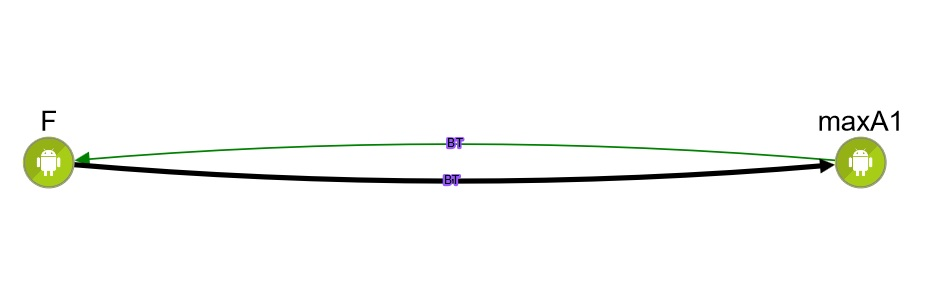
\includegraphics[width=1.0\textwidth]{belege/grosstests/Bilder/Erfolg1.jpg} \\4. Eine
erfolgreich übertragene Nachricht zwischen 2 benachbarten Handys mit
Acknowledgement.

\paragraph{Folgende Beispiele veranschaulichen Nachrichten, die nicht beim Empfänger angekommen sind:}
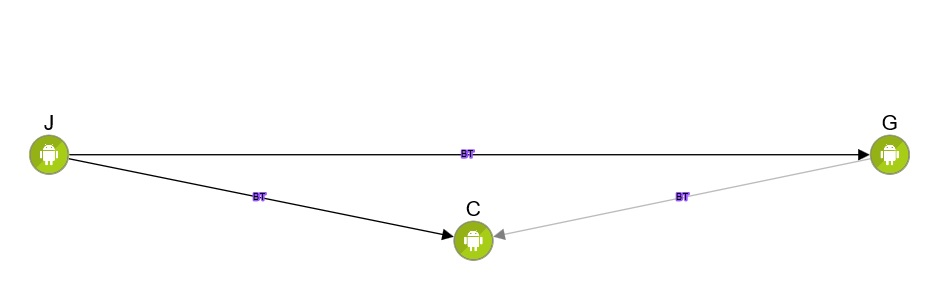
\includegraphics[width=1.0\textwidth]{belege/grosstests/Bilder/Miserfolg6.jpg}\\ 1. J versucht
eine Nachricht zu schicken. Es befinden sich jedoch nur die Handys G und
C in Reichweite, die jedoch nicht der Empfänger sind. G kann daraufhin nur Verbindung mit C herstellen, das
jedoch die Nachricht bereits kennt.\\
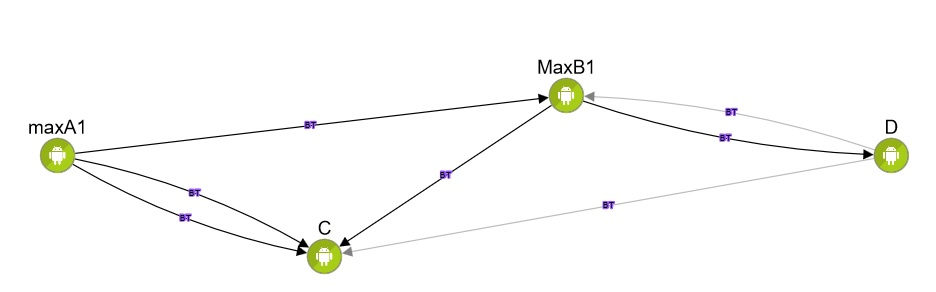
\includegraphics[width=1.0\textwidth]{belege/grosstests/Bilder/Miserfolg5.jpg}\\ 2. A versucht
eine Nachricht zu schicken. Es befinden sich jedoch nur die Handys B und
C in Reichweite. B kann die Nachricht nun noch an D weiterleiten. Dort
bleibt sie jedoch hängen, da D nur noch eine Verbindung zu C findet, das
die Nachricht bereits kennt. A versucht daraufhin in einem Retry die
Nachricht erneut zu schicken, findet aber nun nur noch C.\\
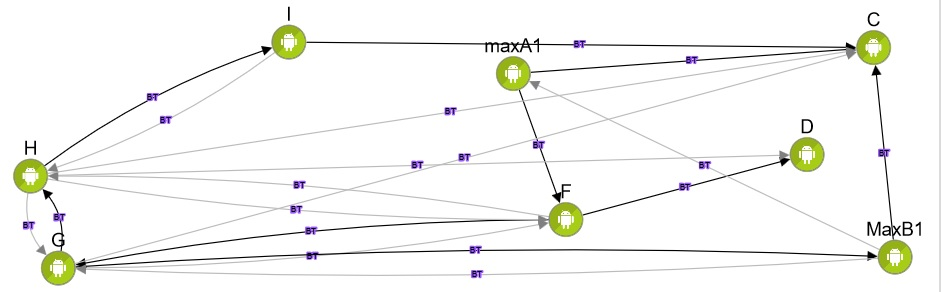
\includegraphics[width=1.0\textwidth]{belege/grosstests/Bilder/Miserfolg4.jpg}\\ 3. An diesem
Beispiel erkennt man, dass alle Handys nah zueinander lagen. Die
Nachricht wird von A verschickt. Sie durchläuft sieben der neun anderen Handys.\\
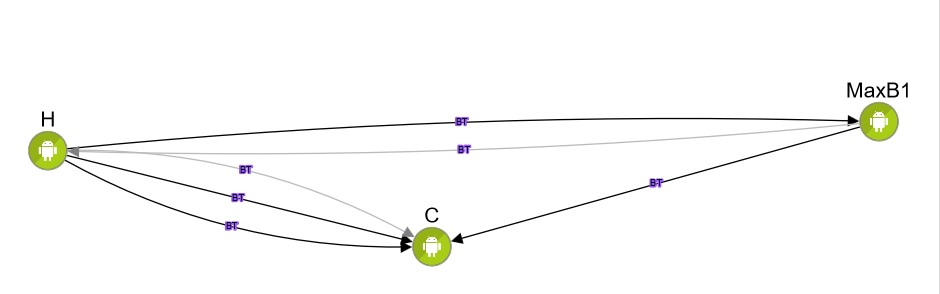
\includegraphics[width=1.0\textwidth]{belege/grosstests/Bilder/Miserfolg3.jpg}\\ 4. H versendet
diese Nachricht. Handy C blockiert jedoch die erfolgreiche Übermittlung
der Nachricht. \\
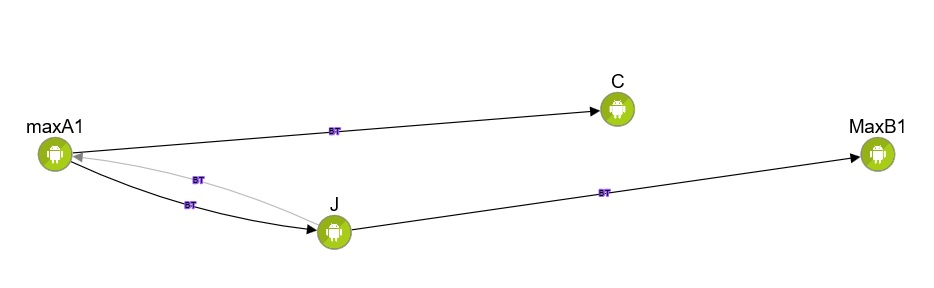
\includegraphics[width=1.0\textwidth]{belege/grosstests/Bilder/Miserfolg2.jpg}\\
5. Auch hier kommt die Nachricht nicht an Handy C vorbei. Auf einem
anderem Pfad schafft sie zwei Hops.\\
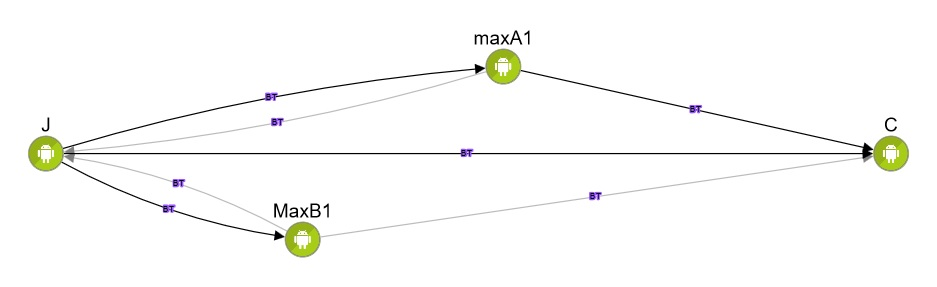
\includegraphics[width=1.0\textwidth]{belege/grosstests/Bilder/Miserfolg1.jpg}\\ 6. J versendet
hier die Nachricht an seine drei Nachbarn. Da jedoch J, A und B (nur) C als
Nachbarn finden, kommt die Nachricht nicht an.\\

\paragraph{Schlussfolgerung aus dem Test:}

Es kamen extrem wenige Nachrichten an. Dies lag daran, dass die Handys
Probleme hatten, sich zu verbinden. Es liegt nahe, dass der
Bluetoothadapter nicht genügend Ports hat um sich mit allen in der Nähe
befindlichen Geräten zu verbinden. Eine Möglichkeit dies zu lösen, wäre
es, sich nicht dauerhaft mit allen Geräten in der Umgebung zu verbinden,
sondern eine Verbindung nach einer Übertragung wieder zu schließen.

Weiterhin gab es Handys, die Nachrichten überhaupt nicht
weitergeleitet haben. Vermutlich war an diesen der Stromsparmodus von
Android aktiv. Ein Beispiel hierfür wäre C.

\paragraph{Verbesserungen bis zum nächsten Test:}

\begin{itemize}
  \tightlist
  \item Die Anzahl der aufzubauenden Verbindungen heruntersetzen.
  \item Ein Test mit mehr anwesenden Personen durchführen um Android daran zu hindern in den Stromsparmodus zu gehen, da dieser nicht ohne Root-Rechte abschaltbar ist.
\end{itemize}


\subsubsection{Ergebnisse Test 2}

Bevor wir Test 2 gestartet haben, haben wir auf allen Handys den
Bluetooth Adapter deaktiviert und erneut aktiviert. Das sollte
eingefrorene Bluetooth Adapter wieder aktivieren. Dieses Vorgehen
basierte auf Erfahrungen von früheren kleinen Tests beim Programmieren.

Im Test 2 haben wir auf 166 Nachrichten 2 erfolgreiche Fälle und 164
Errors.

\paragraph{Folgende Beispiele veranschaulichen die Nachrichten, die beim
Empfänger angekommen sind:}

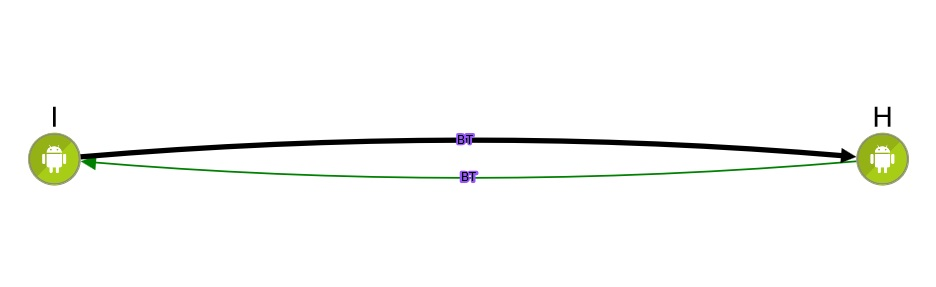
\includegraphics[width=1.0\textwidth]{belege/grosstests/Bilder/Test2Erfolg1.jpg}\\
 1. Nachricht
zwischen zwei benachbarten Handys.\\
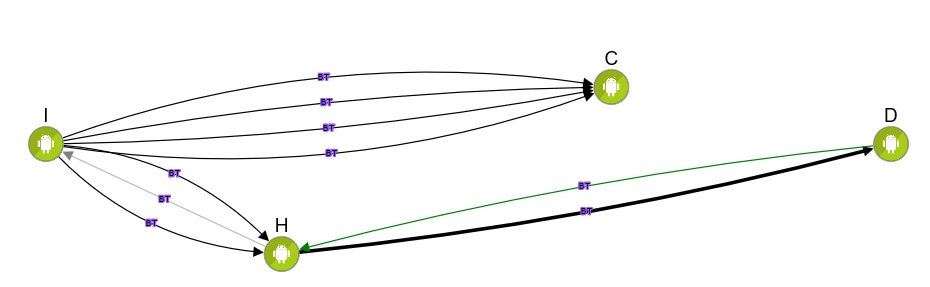
\includegraphics[width=1.0\textwidth]{belege/grosstests/Bilder/Test2Erfolg2.jpg}\\ 2. Nachricht
über einen Hop, die bei einem Retry erfolgreich wurde.\\

\paragraph*{Folgende Beispiele veranschaulichen Nachrichten, die nicht beim
Empfänger angekommen sind:}

\includegraphics[width=1.0\textwidth]{belege/grosstests/Bilder/Test2Misserfolg1.jpg}\\ 1. Das
Handy J hatte während des kompletten Tests keine Verbindung zu einem
Handy aufbauen können.\\
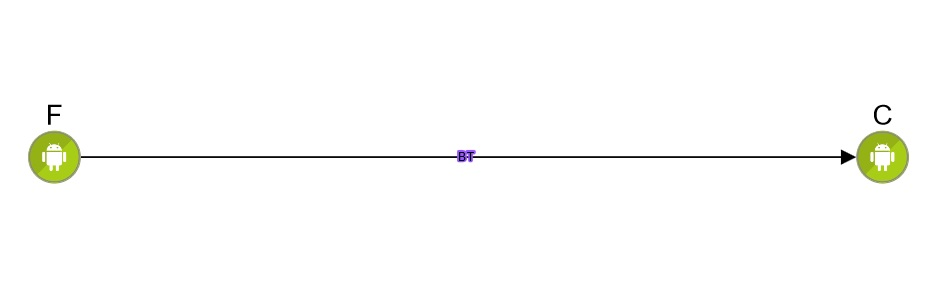
\includegraphics[width=1.0\textwidth]{belege/grosstests/Bilder/Test2Misserfolg3.jpg}\\ 2.
Generell hatten die Handys mehr Probleme Verbindungen aufzubauen.
Dadurch gab es viele Nachrichten, die gar nicht, oder nur bis zum
Nachbarn weitergeleitet wurden.\\
\includegraphics[width=1.0\textwidth]{belege/grosstests/Bilder/Test2Misserfolg4.jpg} \\3. Das
Handy B versucht eine Nachricht zu verschicken, schafft es jedoch nur
bis zu seinen unmittelbaren Nachbarn.\\
\includegraphics[width=1.0\textwidth]{belege/grosstests/Bilder/Test2Misserfolg5.jpg}\\
\includegraphics[width=1.0\textwidth]{belege/grosstests/Bilder/Test2Misserfolg6.jpg}\\ 4. und
5. Nachrichten wurden von einem Handy verschickt und schafften es eine
Nachricht mehr als einen Hop zu übertragen. Dies passierte bei diesem
Test bereits sehr selten.\\

\paragraph{Schlussfolgerung aus dem Test:}

Dieser Test zeigte, dass bereits Abstände von circa 5 Metern einen stark
beeinflussenden Faktor haben und extrem viel weniger Verbindungen
aufgebaut wurden als in Test 1.\\

Auch hier gab es wieder Handys, die vermutlich von Android in den
Energiesparmodus versetzt wurden, da diese von niemandem bedient wurden
und nur als Relaisstation gedient haben.

\paragraph{Verbesserungen bis zum nächsten Test:}

Siehe Test 1, keine weiteren Erkenntnisse gewonnen.


\subsubsection{Ergebnisse Test 3}

Da die Ergebnisse nicht unseren Erwartungen entsprachen, beschlossen wir
den Test hier abzubrechen. Der letzte Test unterliegt schwereren
Bedingungen und bringt dadurch nur bei Erfolg von Test 1 oder 2 bessere
Ergebnisse.


\clearpage

\subsection{Durchführung des Großtests 2}

Nach dem letzten Test wurde der Code so erweitert, dass Bluetooth nur
noch 4 Verbindungen gleichzeitig aufbaut und in regelmäßigen Abständen
alte Verbindungen fallen lässt. Das hindert den Bluetooth Adapter zu
schnell zu überlasten.

Außerdem wurden weitere Kommilitonen darum gebeten am Test teilzunehmen.
Insgesamt wurde der Test von 9 Personen mit 14 Handys ausgeführt.

Die Benennung der Handys wurde den einzelnen Personen überlassen. Es
wurde dafür gesorgt, dass alle Handys den Kontakt der anderen Handys
kennen.


\subsubsection{Ergebnisse Test 1}

Wir haben auf 167 Nachrichten 8 erfolgreiche Fälle und 159 Errors.

\paragraph{Folgende Beispiele veranschaulichen Nachrichten, die beim
Empfänger angekommen sind:}

\includegraphics[width=1.0\textwidth]{belege/grosstests/Bilder/Grosstest2/Test1Erfolg2.jpg}
1. mnex2 sendet eine Nachricht an F2. Diese kommt erst nach einer
Retransmission an. Das Acknowledgement kommt auch erst beim 2. Versuch
an.

\includegraphics[width=1.0\textwidth]{belege/grosstests/Bilder/Grosstest2/Test1Erfolg1.jpg}

2. Hier sendet a2 eine Nachricht an F2. Da F2 ein Nachbar ist, kommt die
Nachricht direkt an. A2 versucht gleichzeitig auch noch einen weiteren
Weg, der jedoch nach einem Hop verloren geht.

\includegraphics[width=1.0\textwidth]{belege/grosstests/Bilder/Grosstest2/Test1Erfolg3.jpg}

3. In dieser Nachricht sendet 3 an 2. Die Nachricht wird erfolgreich über 1
geschickt. 1 sendet die Nachricht gleichzeitig auch noch an a2.

\paragraph{Folgende Beispiele veranschaulichen Nachrichten, die nicht beim
Empfänger angekommen sind:}

\includegraphics[width=1.0\textwidth]{belege/grosstests/Bilder/Grosstest2/Test1Misserfolg2.jpg}

1. Bei diesem Test kam es häufig zur Situation, dass Handys überhaupt keine
Verbindung mit anderen Geräten herstellen konnten. Dies kann daran
liegen, dass die Geräte in der näheren Umgebung bereits 4 Verbindungen
offen hatten, oder dessen Bluetooth durch frühere Transmissions
überlastet war.

\includegraphics[width=1.0\textwidth]{belege/grosstests/Bilder/Grosstest2/Test1Misserfolg1.jpg}

2. Hier sendet a2 eine Nachricht, die jedoch nur über einen Hop
weitergeleitet wird und deshalb nicht ankommt.

\includegraphics[width=1.0\textwidth]{belege/grosstests/Bilder/Grosstest2/Test1Misserfolg3.jpg}

3. Auch hier sendet a2 eine Nachricht, die über die Hops F2, Nightfire und
2 läuft, dort jedoch verloren geht.

\paragraph{Schlussfolgerung aus dem Test:}

Die Einschränkung auf 4 Verbindungen pro Bluetooth-Gerät scheint nicht
erfolgreich gewesen zu sein. Der Bluetoothadapter scheint immer noch
sehr schnell zu überlasten. Die Einschränkung führt außerdem noch dazu,
dass nicht alle Handys in der Umgebung erreicht werden, da bereits 4
Verbindungen bestehen, oder versucht aufgebaut zu werden.\\

Es bestand kein Grund zur Annahme, dass Verbindungen bei diesem Test
nicht zustande gekommen sind, weil ein Handy in den Standby-Modus
gegangen ist.


\subsubsection{Ergebnisse Test 2}

Wir haben auf 227 Nachrichten 20 erfolgreiche Fälle und 7 Errors.

\paragraph{Folgende Beispiele veranschaulichen Nachrichten, die beim Empfänger angekommen sind:}

\includegraphics[width=1.0\textwidth]{belege/grosstests/Bilder/Grosstest2/Test2Erfolg1.jpg}

1. Die Verbindung zwischen mnex2 und Sven bestand über den ganzen Test.
Über diese Verbindung gingen 13 Nachrichten.

\includegraphics[width=1.0\textwidth]{belege/grosstests/Bilder/Grosstest2/Test2Erfolg3.jpg}

2. G3n3siS sendet eine Nachricht an Sven. Diese wird erfolgreich an a2
übermittelt, welches diese dann an Sven weiterleitet. Das
Acknowledgement kommt jedoch nicht mehr zurück.

\includegraphics[width=1.0\textwidth]{belege/grosstests/Bilder/Grosstest2/Test2Erfolg4.jpg}

3. Nightfire sendet eine Nachricht an mnex2.

\paragraph{Folgende Beispiele veranschaulichen Nachrichten, die nicht beim Empfänger angekommen sind:}

\includegraphics[width=1.0\textwidth]{belege/grosstests/Bilder/Grosstest2/Test2Misserfolg1.jpg}

1. Im Verhältnis zu Test 1 gab es noch häufiger die Situation, dass Handys
gar nicht mit anderen Geräten verbunden sind.

\includegraphics[width=1.0\textwidth]{belege/grosstests/Bilder/Grosstest2/Test2Misserfolg2.jpg}

2. G3n3siS verschickt eine Nachricht, die jedoch von seinem Nachbarn
Nightfire nicht weitergeleitet wird.

\includegraphics[width=1.0\textwidth]{belege/grosstests/Bilder/Grosstest2/Test2Misserfolg3.jpg}

3. Nightfire baut eine Verbindung zu mehreren Nachbargeräten auf, die sich
jedoch nur gegenseitig finden.

\paragraph{Schlussfolgerung aus dem Test:}

Die Anzahl der erfolgreichen Verbindungen ist sehr stark von der
funktionierenden Verbindung zwischen mnex und Sven beeinflusst.

Die Tatsache, dass extrem viele Geräte überhaupt keine Verbindung mehr
aufbauen konnten, unterstützt die Aussage, die bereits nach Test 1
getroffen wurde, dass die Limitierung der Slots nicht zielführend war.


\subsubsection{Ergebnisse Test 3}

Da wir gemerkt haben, dass die Limitierung der Slots auf 3 nicht
zielführend war, haben wir diese für Test 3 wieder rückgängig gemacht.

Wir haben auf 164 Nachrichten 11 erfolgreiche Fälle und 153 Errors.

\paragraph{Folgende Beispiele veranschaulichen Nachrichten, die beim Empfänger angekommen sind:}

\includegraphics[width=1.0\textwidth]{belege/grosstests/Bilder/Grosstest2/Test3Erfolg1.jpg}

\includegraphics[width=1.0\textwidth]{belege/grosstests/Bilder/Grosstest2/Test3Erfolg2.jpg}

1 und 2. Nachrichten die zu einem benachbarten Empfänger gesendet werden.

\includegraphics[width=1.0\textwidth]{belege/grosstests/Bilder/Grosstest2/Test3Erfolg3.jpg}

3. Mnex sendet eine Nachricht an Sven diese kommt jedoch erst nach dem
zweiten Versuch an. Auch das Acknowledgement benötigt zwei Versuche.

\paragraph{Folgende Beispiele veranschaulichen Nachrichten, die nicht beim Empfänger angekommen sind:}

\includegraphics[width=1.0\textwidth]{belege/grosstests/Bilder/Grosstest2/Test3Misserfolg1.jpg}

1. G3n3siS sendet eine Nachricht. Diese geht jedoch nach zwei Hops verloren.\\

\includegraphics[width=1.0\textwidth]{belege/grosstests/Bilder/Grosstest2/Test3Misserfolg2.jpg}

2. Das wohl häufigste Beispiel des dritten Tests. Zwei benachbarte Geräte
schaffen es, eine Verbindung aufzubauen. Das zweite Handy schafft es
jedoch dann nicht, die Nachricht weiterzuleiten.

\includegraphics[width=1.0\textwidth]{belege/grosstests/Bilder/Grosstest2/Test3Misserfolg3.jpg}

3. Auch hier gab es Fälle, in denen ein Handy keine Verbindung mit einem anderen Gerät aufbauen konnte. Dies passiert jedoch deutlich seltener als bei Test 1 und 2.

\paragraph{Schlussfolgerung aus dem Test:}

Der dritte Test ist besser gelaufen als der 2. Da die Entfernung einen
erschwerenden Faktor darstellt, kann davon ausgegangen werden, dass die
Verbesserung dadurch zustande kam, dass wir die Slots nicht mehr
limitieren.

\subsubsection{Ausblick und zukünftige Tests}

Im Auftraggebertreffen wurde entschieden, dass keine weiteren
Verbesserungen am Bluetooth-Code durchgeführt werden sollen. Die Begründung
hierfür ist, dass die Implementierung des Bluetooth-Stacks wohl
teilweise fehlerhaft ist.

Die Lösung hierfür ist eine eigene Implementierung des Bluetooth-Stacks.
Diese soll jedoch im Rahmen einer Bachelorarbeit geschrieben werden, da
dies nicht Bestandteil des Bachelorpraktikums ist.

Da sich deshalb in der Funktionalität der Nachrichtenübertragung nichts
mehr ändern wird, haben wir auf einen dritten Großtest verzichtet.



\clearpage
\section{Erweiterbarkeit}

Während der Entwicklung der Anwendung haben wir zusammen mit unserem Auftraggeber als weiteres Qualitätsziel erkannt, dass die App leicht um weitere Übertragungswege erweiterbar sein soll. Zu diesem Zweck existiert ein Interface `IProtocol`.

Die Erweiterung der Anwendung um einen weiteren Übertragungsweg wird im folgenden anhand des beispielhaften EchoProtocol dokumentiert, welches Nachrichten direkt an den Absender zurückschickt. Dazu sind folgende Schritte notwendig:

\subsection{Entwicklung einer neuen Klasse `EchoProtocol`}

Der Entwickler muss zunächst eine neue Klasse EchoProtocol implementieren. Die neue Klasse muss das Interface `IProtocol` implementieren.

\begin{lstlisting}[language=Java]
app/src/main/java/de/tudarmstadt/informatik/bp/bonfirechat/network/IProtocol.java

public interface IProtocol {
    void sendPacket(Packet packet, Peer peer);
    void setIdentity(Identity identity);
    void setOnPacketReceivedListener(OnPacketReceivedListener listener);
    void setOnPeerDiscoveredListener(OnPeerDiscoveredListener listener);
    boolean canSend();
    void shutdown();
}
\end{lstlisting}

Eine beispielhafte Implementierung des EchoProtocol sieht wie folgt aus:

\begin{lstlisting}[language=Java]
app/src/main/java/de/tudarmstadt/informatik/bp/bonfirechat/network/EchoProtocol.java

public class EchoProtocol extends SocketProtocol {

    private static final String TAG = "EchoProtocol";

    private Identity mIdentity;
    private OnPacketReceivedListener mOnPacketReceivedListener;
    private OnPeerDiscoveredListener mOnPeerDiscoveredListener;

    public EchoProtocol(Context ctx) {
    }

    // ###########################################################################
    // ###    Implementation of IProtocol
    // ###########################################################################

    void setIdentity(Identity identity) {
         mIdentity = identity;
    }
    void setOnPacketReceivedListener(OnPacketReceivedListener listener) {
         mOnPacketReceivedListener = listener;
    }
    void setOnPeerDiscoveredListener(OnPeerDiscoveredListener listener) {
         mOnPeerDiscoveredListener = listener;
    }
    
    @Override
    public void sendPacket(Packet packet, Peer peer) {
        Log.d(TAG, "echoing packet via EchoProtocol");
        mOnPacketReceivedListener.onPacketReceived(this, packet);
    }

    @Override
    public boolean canSend() {
        // this dummy protocol is always ready to send messages
        return true;
    }

    @Override
    public void shutdown() {
    }
}

\end{lstlisting}


\subsection{Eintragen des neuen Protokolls im ConnectionManager}

Damit das Protokoll beim Start der Anwendung instanziiert werden kann, muss es in der Liste der registrierten Protokolle im ConnectionManager aufgeführt werden:
\begin{lstlisting}[language=Java]
app/src/main/java/de/tudarmstadt/informatik/bp/bonfirechat/network/ConnectionManager.java

public class ConnectionManager extends NonStopIntentService {

    // ...
    
    static final Class[] registeredProtocols = new Class[]{
            BluetoothProtocol.class,
            WifiProtocol.class,
            GcmProtocol.class,
            EchoProtocol.class   // new
            };

\end{lstlisting}

Außerdem sollte in den App-Einstellungen ein neues Auswahlfeld eingefügt werden, sodass der Benutzer das Protokoll ein- und ausschalten kann.

\begin{lstlisting}
app/src/main/res/xml/preferences.xml

        <CheckBoxPreference android:key="enable_EchoProtocol" android:defaultValue="true"
            android:title="@string/use_echo_protocol"></CheckBoxPreference>
\end{lstlisting}




\subsection{Quellcode BluetoothProtocol}

Als Beispiel für eine vollständige Implementierung eines Übertragungsprotokolls führen wir hier noch den Quellcode des BluetoothProtocol sowie der Elternklasse SocketProtocol, die einige Methoden enthält, die von allen bisherigen Protokoll-Implementierungen verwendet werden, und ihrerseits von IProtocol erbt, an.

Der Quellcode soll auch Beleg dafür sein, dass wir durch unsere QS-Maßnahmen eine gute Codequalität erreicht haben.

\subsubsection{SocketProtocol}
\lstinputlisting[language=Java]{../BonfireChat/app/src/main/java/de/tudarmstadt/informatik/bp/bonfirechat/network/SocketProtocol.java}

\subsubsection{BluetoothProtocol}
\lstinputlisting[language=Java]{../BonfireChat/app/src/main/java/de/tudarmstadt/informatik/bp/bonfirechat/network/BluetoothProtocol.java}




